%% LyX 1.3 created this file.  For more info, see http://www.lyx.org/.
%% Do not edit unless you really know what you are doing.
\documentclass[10pt,letterpaper,twocolumn,english]{article}
\usepackage{ae}
\usepackage{aecompl}
\usepackage[T1]{fontenc}
\usepackage[latin1]{inputenc}
\usepackage{float}
\usepackage{amsmath}
\usepackage{graphicx}
\usepackage{amssymb}

\makeatletter

%%%%%%%%%%%%%%%%%%%%%%%%%%%%%% LyX specific LaTeX commands.
\newcommand{\noun}[1]{\textsc{#1}}
%% Because html converters don't know tabularnewline
\providecommand{\tabularnewline}{\\}
\floatstyle{ruled}
\newfloat{algorithm}{tbp}{loa}
\floatname{algorithm}{Algorithm}

%%%%%%%%%%%%%%%%%%%%%%%%%%%%%% User specified LaTeX commands.
\usepackage{url}

\newcommand{\inlinedef}[1]{\emph{#1}\index{#1}\glossary{#1}}
\newcommand{\sphericaltri}{\textcircled{$\triangle$}}

\usepackage{babel}
\makeatother
\begin{document}

\title{The Theory and Practice of Non-Rigid Surface Warping}


\author{Steven M. Robbins}

\maketitle

\newcommand{\Real}{\mathbb{R}}

\newcommand{\Rthree}{\mathbb{R}^{3}}

\newcommand{\Stwo}{\mathbb{S}^{2}}



\section{Introduction}

Surface registration is a procedure that produces a spatial mapping
from one surface, which we call the \emph{source} surface, to a second,
\emph{target}, surface. This manual is not a treatise on surface registration
(see, e.g. \cite{robbins03:phd}) but only documents the specific
theory and practice underlying \noun{surftracc}. 


\section{Input Data}

The input to surface registration is a pair of surfaces such as those
generated from a 3D MR image using software such as \noun{asp}/\noun{clasp}\cite{macdonald00:cortical-surfaces}.
In adition, a feature data function for each surface is required.


\subsection{Surface Description}

Each input surface must be a triangulated polyhedral surface, also
called a \emph{mesh}. Further, \noun{surftracc} assumes that the
surface has a very specific structure as follows.

First of all, \noun{surftracc} requires that the mesh represent
a topological sphere, i.e. a closed surface that bounds a finite volume
of space.

A common way to refine a mesh is by quadrisection, in which each triangle
is replaced by four triangles by joining the midpoints of the three
edges, as shown.

\begin{center}\includegraphics{quadrisection.eps}\end{center}

In addition to being a topological sphere, \noun{surftracc} requires
that the mesh graph be a repeated quadrisection of an icosahedron,
the graph with 20 triangular faces and 12 vertices each of degree
five. Each quadrisection increases the number of faces by a factor
of four. The following table shows the number of faces and vertices
produced by repeated quadrisection.

\begin{center}\begin{tabular}{|c|c|c|}
\hline 
\# Quadrisections&
\# Faces&
\# Vertices\tabularnewline
\hline
\hline 
0&
20&
12\tabularnewline
\hline 
1&
80&
42\tabularnewline
\hline 
2&
320&
162\tabularnewline
\hline 
3&
1280&
642\tabularnewline
\hline 
4&
5120&
2562\tabularnewline
\hline 
5&
20480&
10242\tabularnewline
\hline 
6&
81920&
40962\tabularnewline
\hline 
7&
327680&
163842\tabularnewline
\hline
\end{tabular}\end{center}

Note that ASP/CLASP outputs surfaces of the form required by \noun{surftracc}.


\subsection{Match Feature}

Along with each surface, we need data to determine how the surfaces
match. The basic idea is to define a scalar \emph{feature} function
on each surface such that a matching region on the source and target
have a similar feature pattern. The feature values needn't match exactly
since, as described below, we use a correlation similarity measure
to drive the optimization.

The feature function is defined in a piecewise-linear fashion by providing
the function value at each vertex. At other points on the surface,
the function is interpolated from the 3 values at the triangle vertices.
This interpolation is described in more detail later.

We next describe two geometric feature functions that can be used
for registration: mean curvature and crown distance transform.


\subsubsection{Curvature}

The mean surface curvature is a popular choice for match feature since
gyral crowns and sulcal fundii have curvature of different sign. So
matching curvature should match gyrus to gyrus and sulcus to sulcus.

This Figure shows the value of mean curvature evaluated (using \cite{taubin95:estimating-curvature})
at each vertex of the cortical surface.

\begin{center}\begin{tabular}{cc}
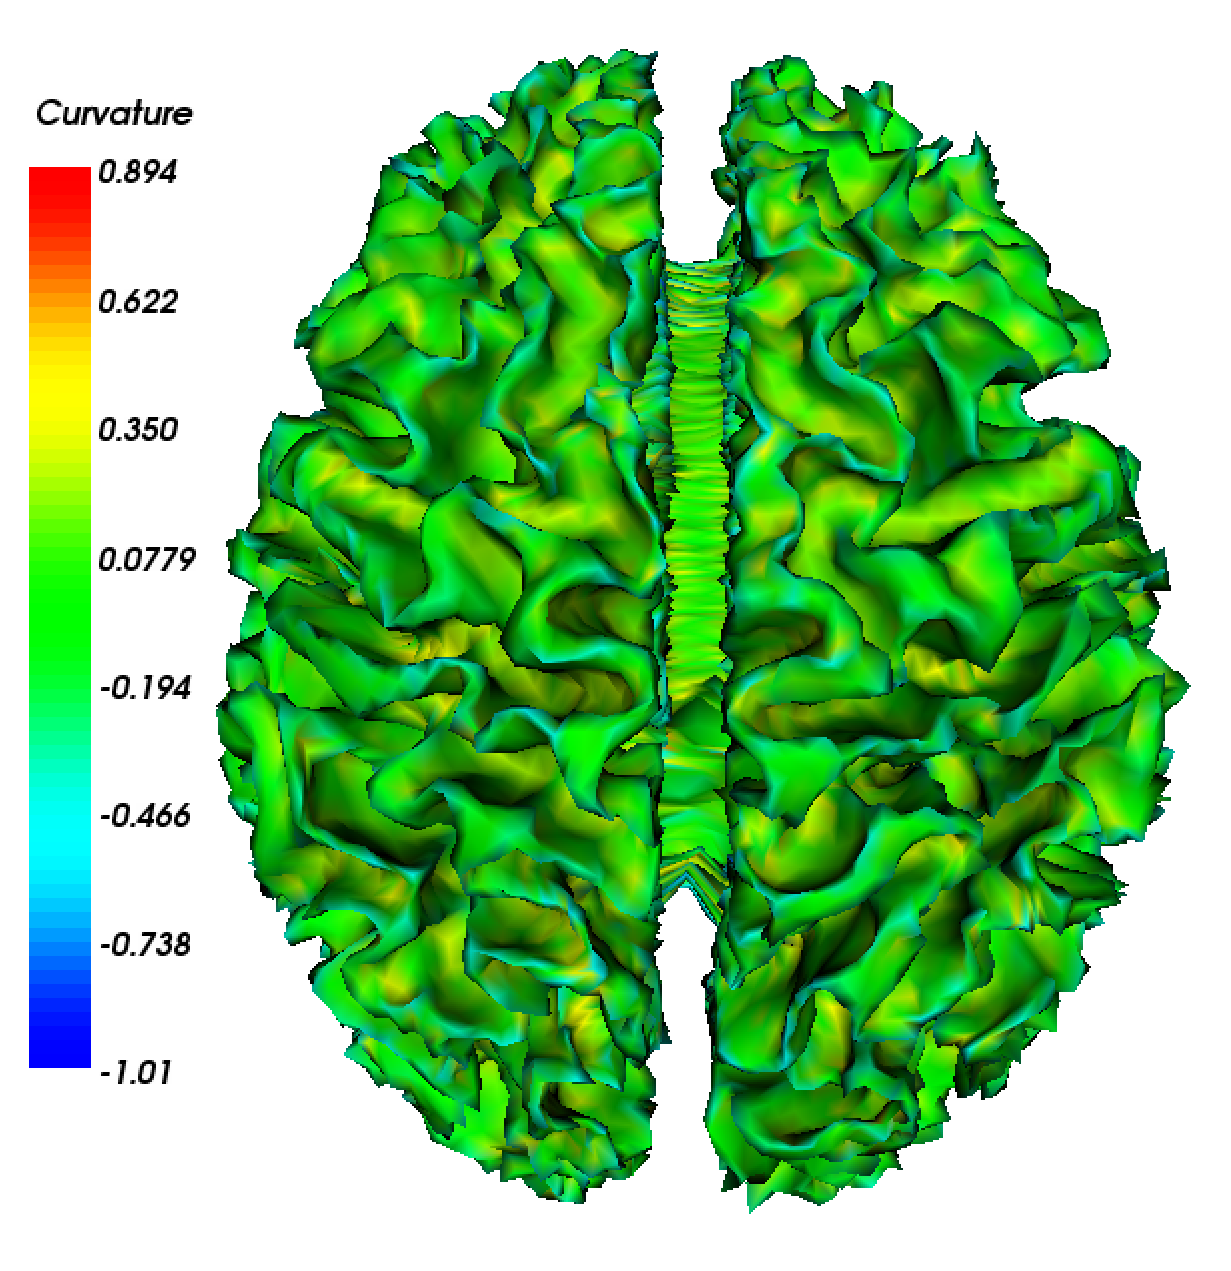
\includegraphics[%
  width=0.45\linewidth,
  keepaspectratio]{mean-cortex-top.ps}&
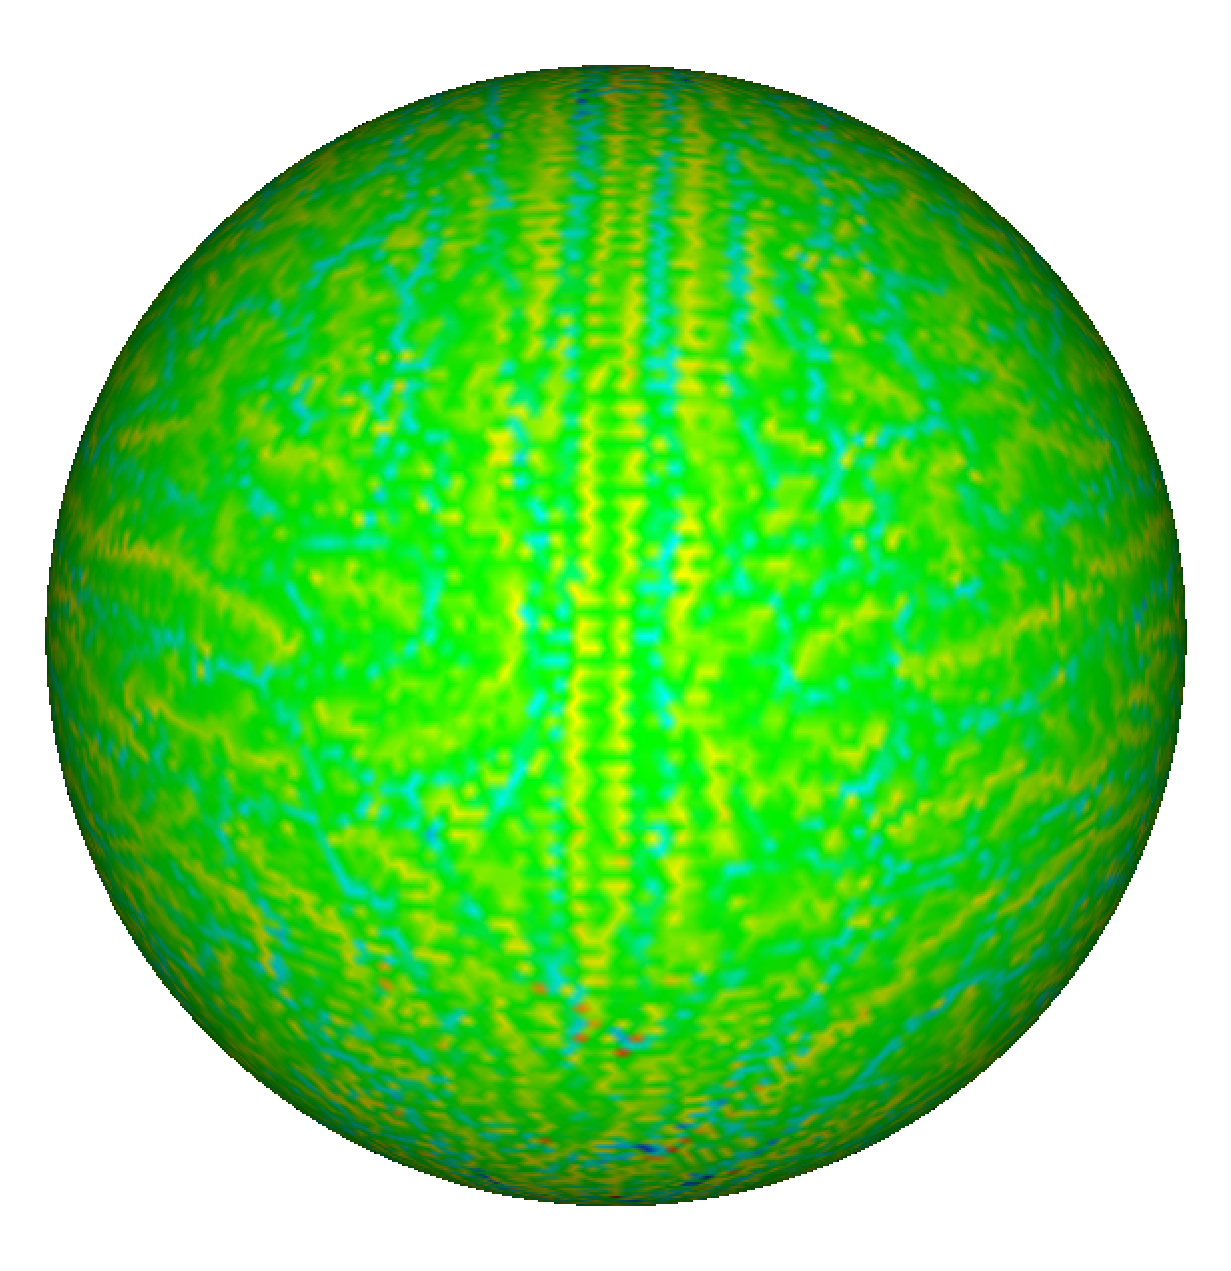
\includegraphics[%
  width=0.45\linewidth,
  keepaspectratio]{mean-sphere-top.ps}\tabularnewline
\end{tabular} \end{center}

Since sulcal fundi and gyral crowns have mean curvature of opposite
sign, registration based on matching mean curvature should tend to
match sulcus to sulcus and gyrus to gyrus. However, there is evidently
a lot of noise in the curvature map as well, due to small-scale oscillations
in the mesh vertex positions, so the data needs to be smoothed when
used for registration, either by smoothing the surface before computing
the curvature, or by directly averaging function values in a neighbourhood
of each vertex.


\subsubsection{Crown Distance Transform}

The intuition behind this feature, like that of mean curvature, is
that it is desirable to match points along the crown of a gyrus on
the source surface with points along the crown of a gyrus in the target
surface. Similarly, the fundus of a sulcus should match the fundus
of a sulcus. In contrast to matching by mean curvature, other points
on the bank of a sulcus are matched according to their fractional
distance towards the bottom of the sulcus, e.g. a vertex halfway down
the sulcus in the source mesh should match a point halfway down the
target sulcus.

Suppose vertex $v$ is located in a sulcus of the source mesh. Consider
two shortest geodesic paths, one from $v$ to the gyral crown and
the other from $v$ to the fundus. Let the length of the first of
these paths be $S(v)$ and let $S_{D}(v)$ be the sum of the two path
lengths. Distance $S_{D}(v)$ can be regarded as the depth of the
sulcus along a path through $v$. Let $R$ and $R_{D}$ be the analogous
distance functions for the target surface. The fractional depth of
vertex $v$ on the source mesh is $S(v)/S_{D}(v)$.

\begin{center}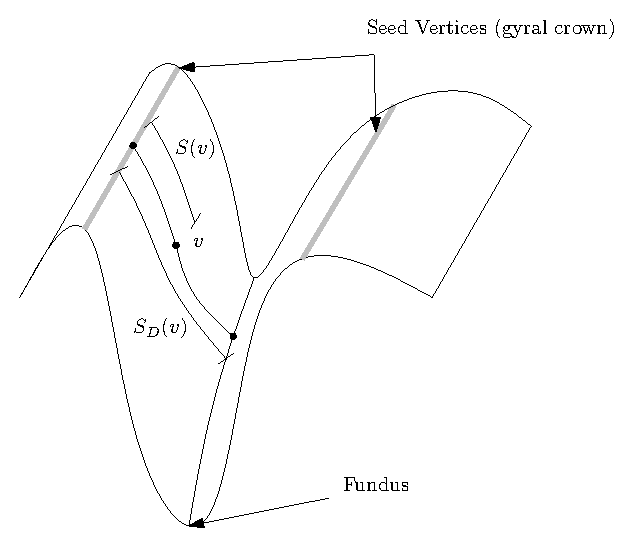
\includegraphics[%
  width=0.9\columnwidth,
  height=0.2\paperwidth,
  keepaspectratio]{fractional-depth.eps}\end{center}

The desired matching is to a point $T(v)$ on the target surface such
that $S(v)/S_{D}(v)\approx R(T(v))/R_{D}(T(v))$, or\begin{equation}
R(T(x))=\alpha(x)+\beta(x)S(x)+\epsilon(x),\label{eq:dt-matching-relation}\end{equation}
 where $\epsilon$ represents random noise, $\beta(x)=R_{D}(T(x))/S_{D}(x)$,
and $\alpha$ should be zero. However, $\alpha$ is left free to compensate
for practical difficulties in computing $S(x)$ and $R(x)$. Note
that points near to $v$ should have depth values close to $S_{D}(v)$
and similarly points near $T(v)$ should have depth values close to
$R_{D}(T(v))$. Assuming that $\alpha$ and $\beta$ are slowly-varying
functions, the maximum likelihood estimate for $T$ corresponds to
maximizing the regional correlation coefficient \cite{robbins03:phd}. 

Note that only the gyral crown distance functions, $S$ and $R$ appear
in Equation~\ref{eq:dt-matching-relation} and not $S_{D}$ and $R_{D}$.
Thus, the feature value stored at each vertex is the geodesic \emph{distance
transform} from a set of gyral {}``seed'' vertices, i.e. the length
of the shortest geodesic path from $v$ to a vertex in the seed set.


\paragraph{Seed Points}

The vertices chosen to be the seeds should in principle be all vertices
located on all the gyral crowns. We can identify gyral vertices with
the help of an \emph{$\alpha$-shape} \cite{edelsbrunner94:alpha-shapes},
a discrete geometry notion that can be considered as a relaxation
of the convex hull. The degree of relaxation is controlled by the
parameter $\alpha$ in the following manner. Let $S$ be a set of
points in $\Rthree$. Define an \emph{$\alpha$-ball}%
\footnote{The definition given here follows the Computational Geometry Algorithms
Library (CGAL) \cite{cgal-web}, as the implementation of $\alpha$-shape
provided by CGAL is used. In the original definition of Edelsbrunner
and M�cke, $\alpha$ is the radius of the $\alpha$-ball.%
} to be a closed ball of radius $\sqrt{\alpha}$, i.e. the point set
$\{ x\in\Rthree:||x-p||\le\sqrt{\alpha}\}$, for some $p\in\Rthree$.
The points of $S$ that form the vertices of the $\alpha$-shape of
$S$ are those that lie on the boundary of an $\alpha$-ball with
no point of $S$ on the interior of the $\alpha$-ball. Such vertices
are said to be \emph{$\alpha$-exposed.} Note that convex hull vertices
are always $\alpha$-exposed, since for every point $x$ on the boundary
of a convex set, there exists a ball of radius $\sqrt{\alpha}$ for
any value of $\alpha$ that intersects the convex set only at $x$.
Thus the vertices of the $\alpha$-shape with $\alpha=\infty$ are
the vertices of the convex hull. As $\alpha$ is decreased, more points
become $\alpha$-exposed until at $\alpha=0$ all points are $\alpha$-exposed. 

Using $\alpha$-balls of radius 10 mm (i.e. $\alpha=100$), a value
empirically chosen using visual inspection of the results, produces
good outlines of several major gyri. However, there are also vertices
in the point set lying underneath the brain on the arbitrary {}``cap''
through the brain stem which should not form part of the seed set;
these vertices are masked out as follows. The distance transform is
computed using the convex hull points as the seed vertices and any
vertex with a distance transform value greater than 35 (a value chosen
empirically) is removed from the set of vertices of the $\alpha$-shape.
The remaining vertices form the seed set used for the crown distance
transform feature.


\paragraph{Geodesic Distance}

The distance transform used in practice is an approximation to the
geodesic distance, as computing true geodesic distance is computationally
costly and difficult to code robustly \cite{lanthier01:approx-weighted-shortest-path}.
The approximation is computed using the mesh graph with the weight
for each edge set to the Euclidean length of the edge. An additional
vertex, $s$, is inserted and attached to each seed vertex with a
zero weight edge. Then Dijkstra's single-source shortest path algorithm
\cite{cormen90:intro-algorithms} is run with $s$ as the source vertex.
To improve the accuracy of the approximation the mesh is refined before
running Dijkstra's shortest path algorithm. First, $m$ equally-space
extra points are inserted on each edge, then a new edge is inserted
for each pair of extra points that either (i) are adjacent on an original
edge, or (ii) are on different edges both of which are incident to
a common (original) facet. The approximate shortest path computed
by this algorithm consists of line segments which are either an edge
of the original surface, or cross a facet of the original surface
as shown.

\begin{center}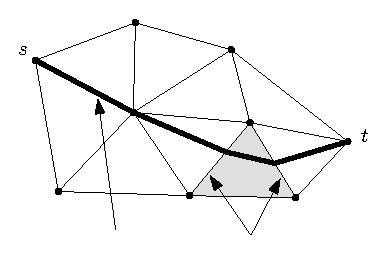
\includegraphics{approximate-path.eps}\end{center}

The crown distance transform from the final seed set is illustrated
below.

\begin{center}\begin{tabular}{cc}
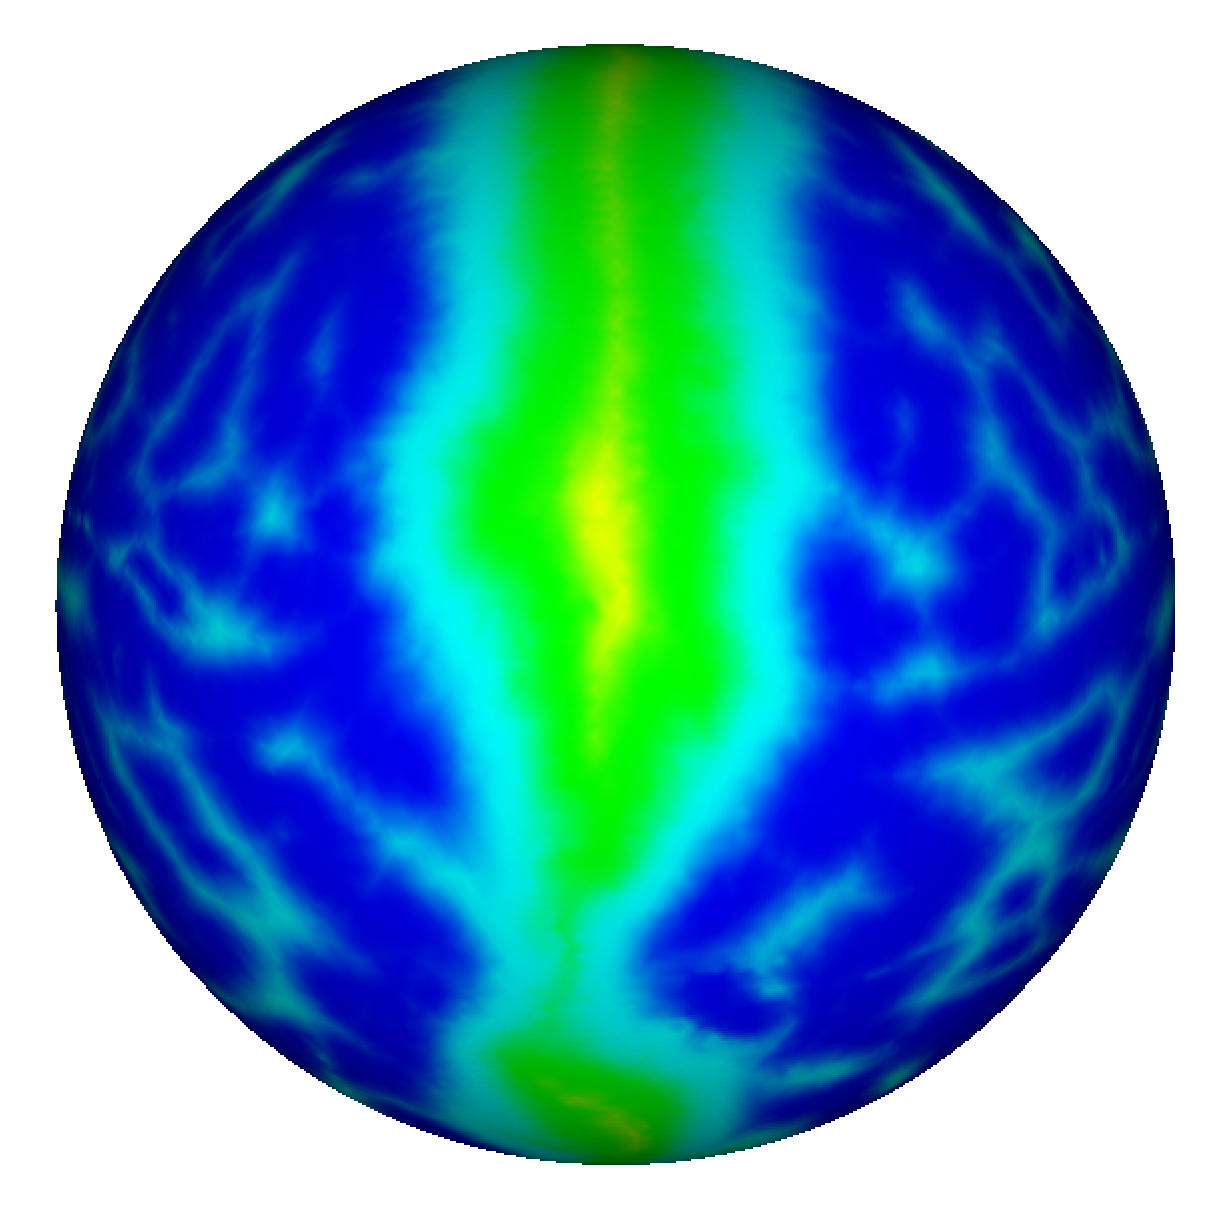
\includegraphics[%
  width=0.4\columnwidth,
  height=0.15\paperwidth,
  keepaspectratio]{sphere-top.ps}&
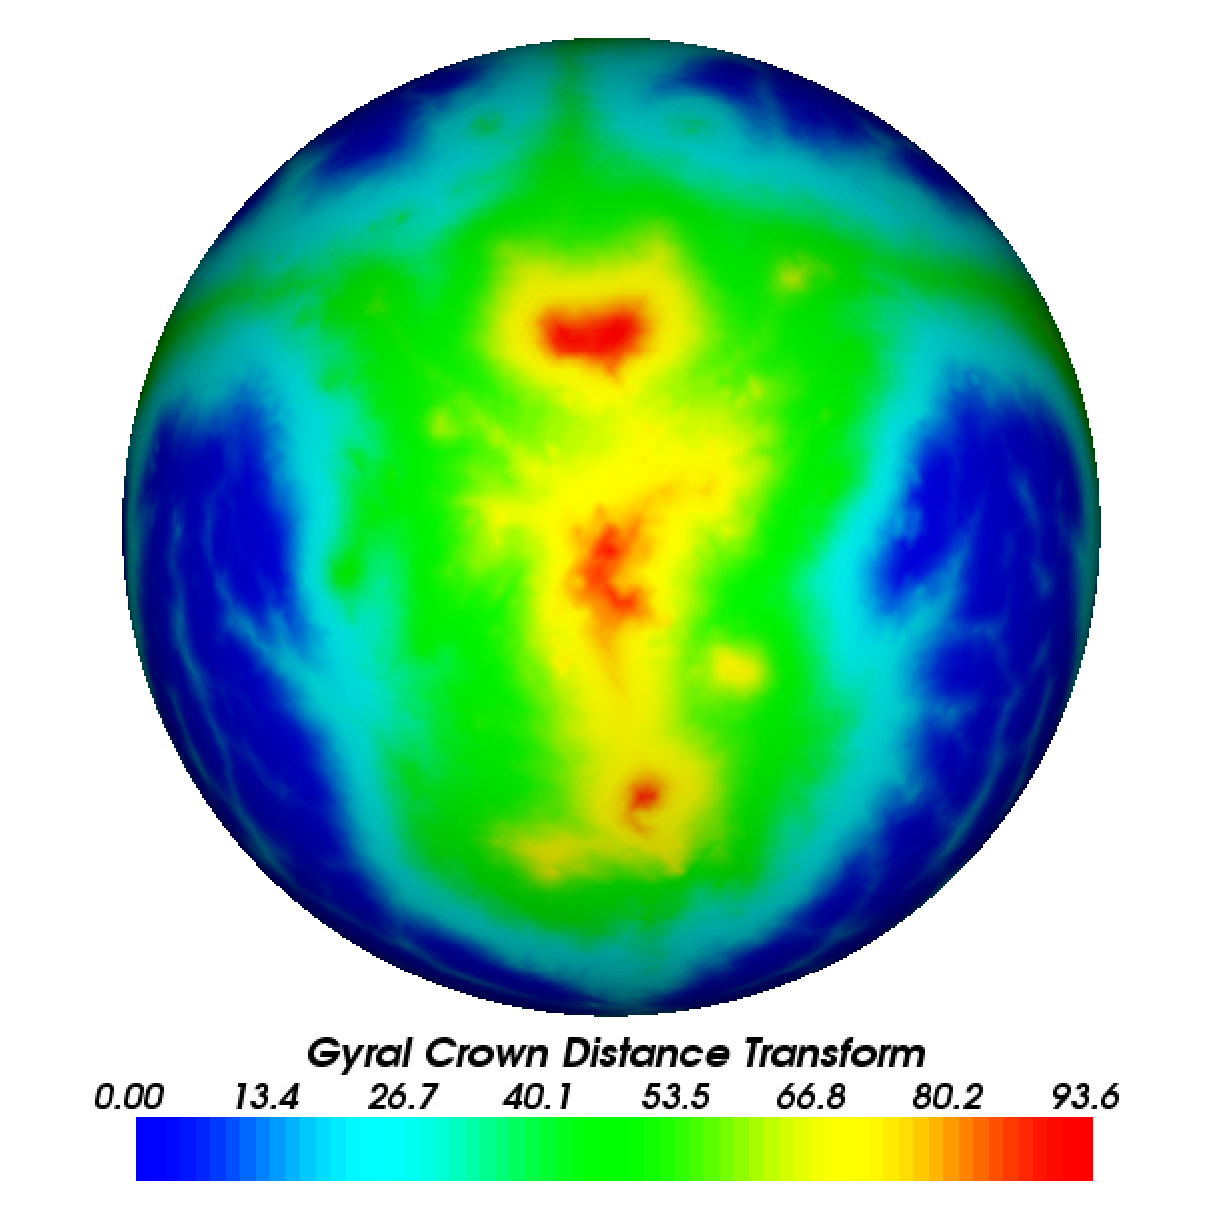
\includegraphics[%
  width=0.4\columnwidth,
  height=0.15\paperwidth,
  keepaspectratio]{sphere-bottom.ps}\tabularnewline
Top&
Bottom\tabularnewline
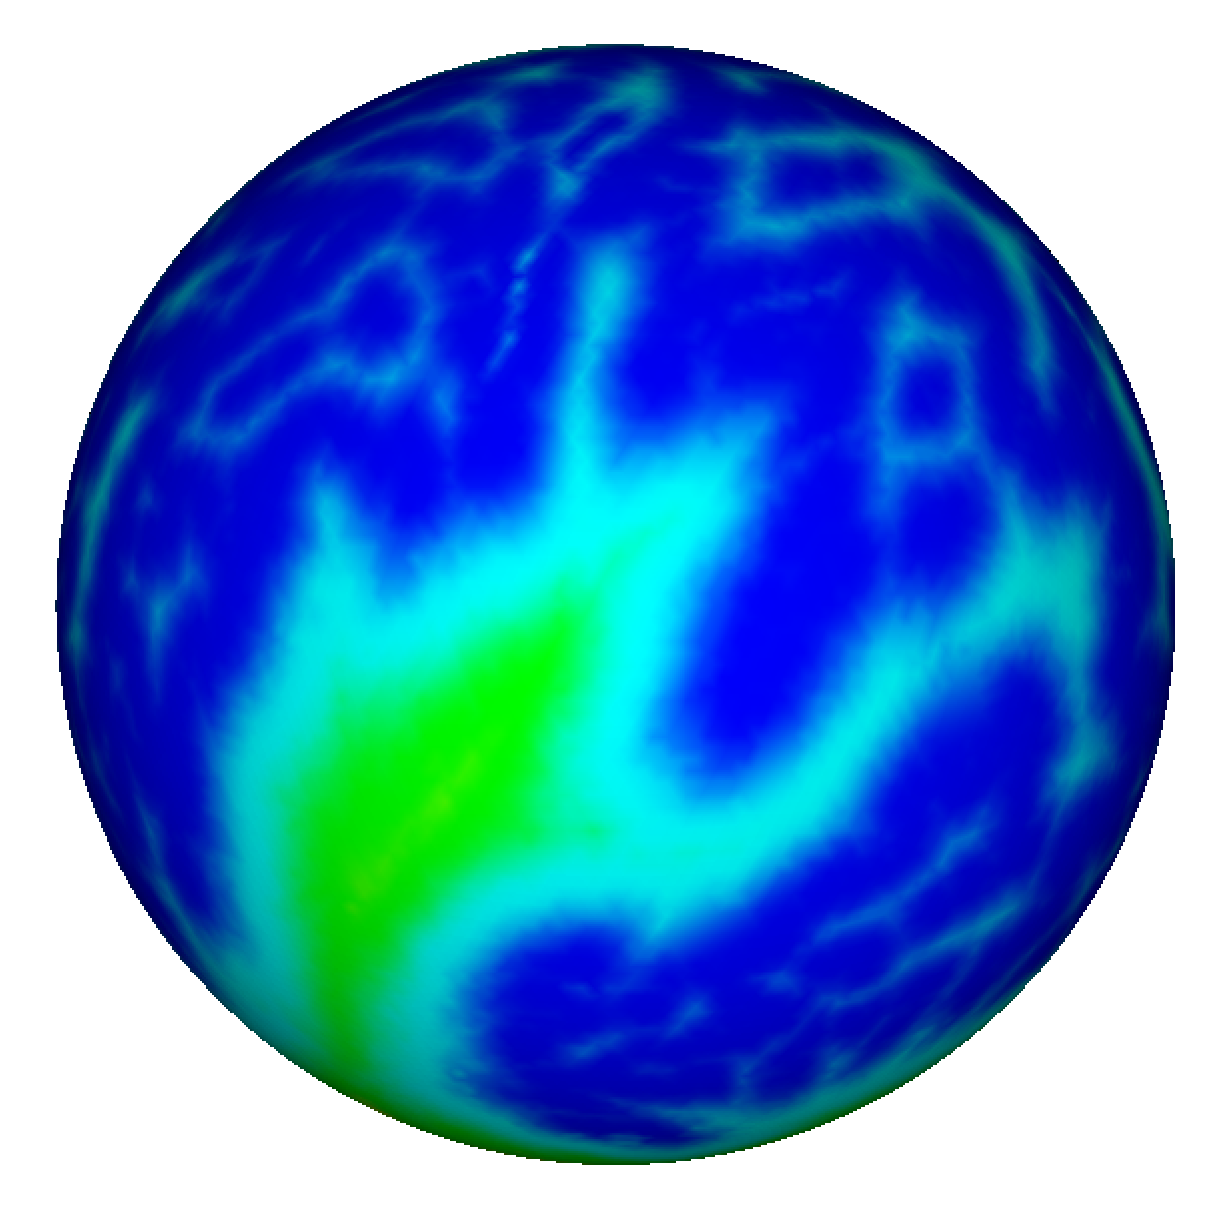
\includegraphics[%
  width=0.4\columnwidth,
  height=0.15\paperwidth,
  keepaspectratio]{sphere-left.ps}&
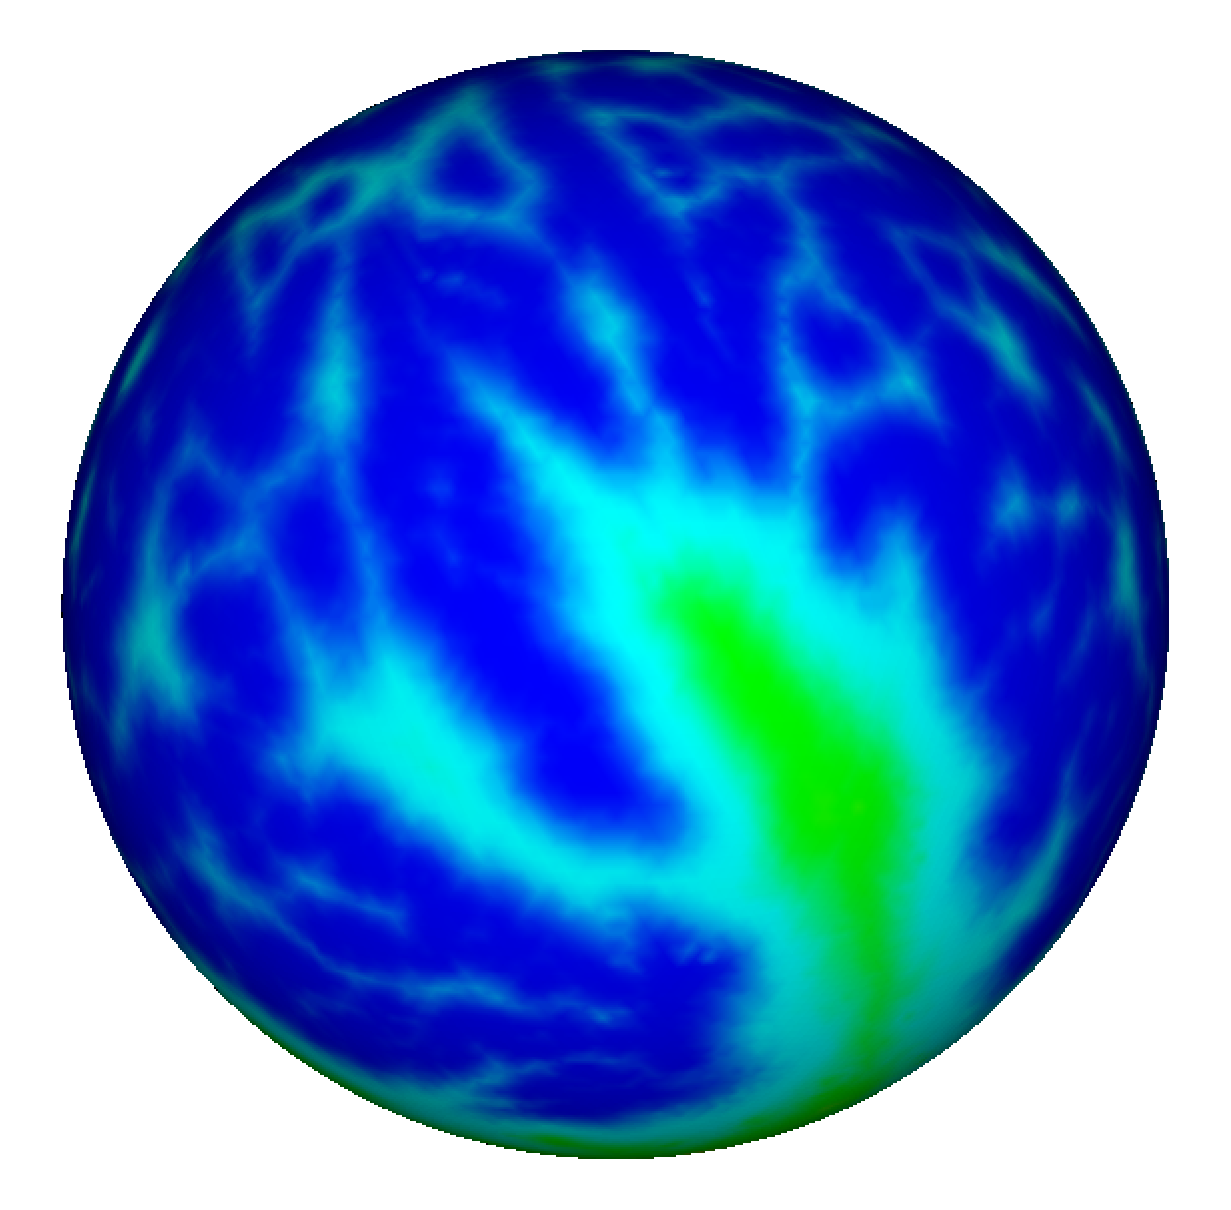
\includegraphics[%
  width=0.4\columnwidth,
  height=0.15\paperwidth,
  keepaspectratio]{sphere-right.ps}\tabularnewline
Left&
Right\tabularnewline
\end{tabular}\end{center}


\section{Triangle Interpolation}

Both the feature data function described above and, ultimately, the
transformation $T$ are defined at mesh vertices and interpolated
across the rest of the surface. We pause to discuss this interpolation
before discussing the optimization used to search for $T$.


\subsection{Scalar Function Interpolation}

Suppose that for a function, $f$, a real value is associated with
each vertex of the mesh, as is the case for the feature function data.
Let $p$ be a point on the mesh and consider what value to assign
$f(p)$. 

If $p$ is a vertex, the vertex value is assigned. 

If $p$ is not a vertex, let $ABC$ be a triangle of the mesh that
contains $p$. There is a unique triple of real values $(\alpha,\beta,\gamma)$
with $\alpha+\beta+\gamma=1$ that satisfies $p=\alpha A+\beta B+\gamma C$.
This triple is known as the \emph{areal coordinates} of $p$ \cite[section 13.7]{coxeter69:intro-geometry}.
We use these values for interpolation, assigning $f(p)=\alpha f(A)+\beta f(B)+\gamma f(C)$.
It is clear that this choice of interpolation (a) is consistent with
the assigned values at vertices $A$, $B$, and $C$, and (b) gives
consistent values along a shared triangle edge no matter which triangle
is used for the interpolation.


\subsection{Triangulation Warping}


\subsubsection{Auxiliary Space}

While it is conceivable to define the mapping $T$ directly on the
input mesh, it is easier to use a simpler auxiliary space instead;
\noun{surftracc} uses the unit sphere. The source mesh, $M_{I}$,
is first mapped to the sphere using an invertible projection map,
$\Pi_{I}$. This projection is given implicitly by the fact that $M_{I}$
is constrained to be a repeated quadrisection of the icosahedron,
as discussed above. The target surface $M_{J}$ is similarly projected
to the sphere by $\Pi_{J}$. The registration algorithm then computes
$T:\Stwo\rightarrow\Stwo$ which, together with the two projection
operations, serves to define map between the two input surface meshes,
denoted $W:M_{I}\rightarrow M_{J}$ in the diagram.

\begin{center}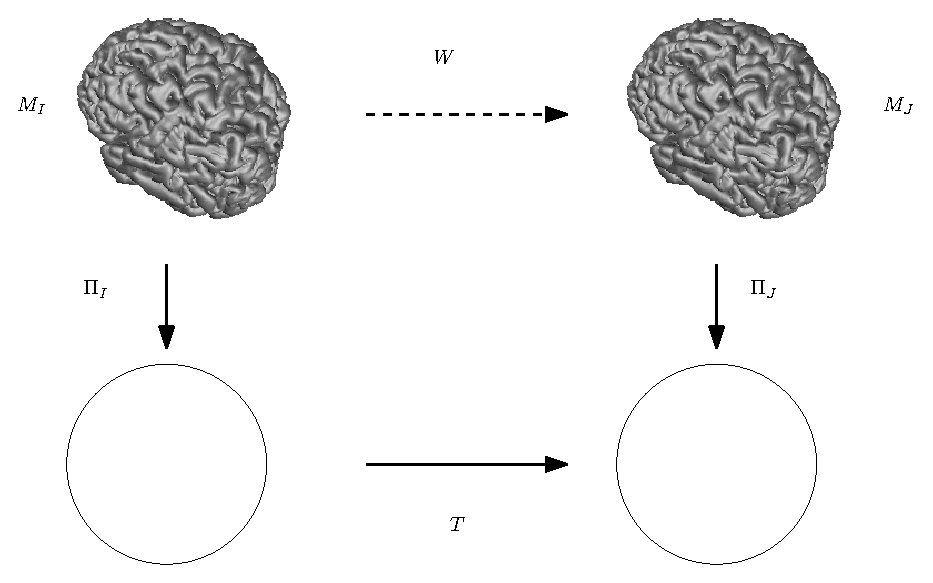
\includegraphics[%
  width=1\columnwidth,
  keepaspectratio]{mappings.eps}\end{center}


\subsubsection{Triangulation Warping on the Sphere}

We discuss now how the sphere-to-sphere mapping, $T:\Stwo\rightarrow\Stwo$
is defined. The basic idea is that the source sphere is partitioned
into spherical triangles, and the mapping under $T$ is given for
each spherical triangle. 


\paragraph{Mapping one Triangle}

Let $A$, $B$, and $C$ be three points on the sphere $\Stwo$ that
are not coplanar with the origin. Using projection from the origin,
i.e. the mapping $x\mapsto x/||x||$, the planar triangle $ABC$ is
put into 1-1 correspondence with a triangular patch of $\Stwo$ bounded
by three shortest geodesics, from $A$ to $B$, from $B$ to $C$,
and from $C$ to $A$. Each geodesic bounding the patch is denoted
an \emph{edge arc}, and the triangular patch of $\Stwo$ is known
as the \emph{spherical triangle} $\sphericaltri ABC$. Given the 1-1
mapping between the planar triangle $\triangle ABC$ and the spherical
triangle $\sphericaltri ABC$, areal coordinates can be used to refer
to either $q=\alpha A+\beta B+\gamma C\in\triangle ABC$ or to $p=q/||q||\in\sphericaltri ABC$.

The mapping of $\sphericaltri ABC$ begins by specifying the positions
of the vertices under the mapping; define $A'\equiv T(A)$, $B'\equiv T(B)$,
and $C'\equiv T(C)$. Define a mapping from point $p$ in spherical
triangle $\sphericaltri ABC$ to point $T(p)$ in spherical triangle
$\sphericaltri A'B'C'$ as follows. First, project $p$ to point $q$
on the planar triangle $ABC$ and compute the areal coordinates of
$q$. We define the corresponding point $q'\in\triangle A'B'C'$ using
$q'\equiv\alpha A'+\beta B'+\gamma C'$. Finally, $q'$ is projected
to point on the sphere, denoted $p'$ and we define $T(p)$ to be
$p'$. 

\begin{center}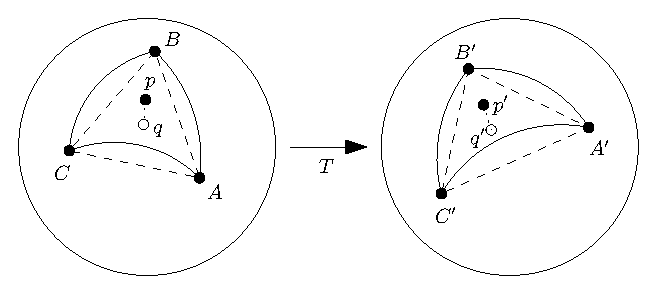
\includegraphics[%
  width=1\columnwidth,
  keepaspectratio]{trianglemap-sphere.eps}\end{center}


\paragraph{Mapping the Entire Sphere}

In order to map the entire sphere, all we need is a partitioning of
the sphere into a set of non-overlapping spherical triangles. For
each triangle, we use the procedure just described to map it. Since
each point of the input sphere is contained in at least one triangle,
a mapping of the sphere is achieved. As is the case when interpolating
real values, the interpolation of $T$ is consistent at vertices and
along edges of each spherical triangle. The overall mapping $T$ is
1-1 and invertible if it satisfies certain conditions \cite{robbins03:phd}.
The main two conditions are that (a) the orientation of each spherical
triangle is preserved (i.e. the triangle is not {}``flipped'') and
(b) for each vertex, the cyclic ordering of its neighbouring vertices
is preserved.

Note that the partitioning of the source sphere is equivalent to finding
a simple triangulated mesh, denoted the \emph{control} mesh, inscribed
in the sphere. The input meshes to \noun{surftracc} provide such
a mesh due to the constraint that they be obtained by repeated quadrisection
of the icosahedron.


\section{Optimizing the Spatial Transformation}

Registration is generally cast in terms of an optimization problem,
in which we seek $T$ that will optimize the match of the feature
function defined on each surface. \noun{surftracc} uses a minimization
with a correlation coefficient-based objective function that penalizes
difference between the feature value at corresponding points on the
surfaces.

In addition, the objective function incorporates a \emph{regularization}
term that penalizes a transformation that is unlikely. Let $S$ and
$R$ be the feature functions on the source and target surfaces, respectively.
The objective function $\Phi$ is expressed as a sum \begin{equation}
\Phi(S,R,T)=\Phi_{D}(S,R,T)+\Phi_{R}(T),\label{eq:obj-is-data-plus-reg}\end{equation}
 and the optimization problem to solve becomes 

\[
T=\arg\min_{T'}\Phi(S,R,T').\]
 

As discussed in the previous section, $T$ is given by specifying
its value at each vertex. The transformation value is a point on $\Stwo$,
which takes two parameters to specify (e.g. latitude and longitude),
so the registration algorithm has two parameters to optimize per vertex.
With so many parameters to estimate (80k on a 40k mesh), it is important
to choose an effective optimization technique. 


\subsection{Two Step Non-Rigid Warping Algorithm}

The complexity is handled by separating the problem into a number
of smaller optimizations \cite{nocedal99:numerical-optimization},
one per vertex. To make this happen, both the data and regularization
terms in Equation \ref{eq:obj-is-data-plus-reg} must be \emph{separable,}
i.e. expressible as a sum of simpler terms. The parameters being optimized
should be partitioned amongst the terms and each term should involve
just a few of the parameters being optimized.

The data term, after discretization to evaluate it on the mesh, is
naturally separable into one term per mesh vertex $v$, involving
only the two values required to specify $T(v)$.

The regularization term can also be made separable by transforming
the problem into two interleaved minimizations. We modify the problem
by introducing a second transformation, $U$. A third term is introduced
into the objective function to link the transformations, resulting
in 

\begin{equation}
\Phi(T,U)=\Phi_{D}(U)+\Psi(T-U)+\Phi_{R}(T),\label{eq:two-step-objective-3d}\end{equation}
where $\Psi$ penalizes difference between $T$ and $U$; we might
use $\Psi(T-U)=\int||T-U||^{2}$, for example. After minimizing over
both $T$ and $U$, the transformation $T$ is returned as the final
solution. In other words, the registration problem solved is\[
\arg\min_{T}\Phi'(T),\]
where \[
\Phi'(T)=\arg\min_{U}\Phi(T,U).\]


The new objective function, Equation \ref{eq:two-step-objective-3d},
has twice as many variables as the original objective function, $\Phi_{D}+\Phi_{R}$.
The registration algorithm proceeds in a sequence of {}``half iteration''
steps. One half iteration fixes the variables that define $T$ while
optimizing $U$ \begin{equation}
U=\arg\min_{U'}\Phi(T,U')=\arg\min_{U'}\Phi_{D}(U')+\Psi(T-U').\label{eq:two-step-U}\end{equation}
The next half iteration fixes the variables that define $U$ while
optimizing $T$\begin{equation}
T=\arg\min_{T'}\Phi(T',U)=\arg\min_{T'}\Psi(T'-U)+\Phi_{R}(T').\label{eq:two-step-T}\end{equation}
 The first step (Expression \ref{eq:two-step-U}) can be seen as finding
a transformation, $U$, that matches the data while remaining close
to the previous solution, $T$ by virtue of $\Psi$. The second step
(Expression \ref{eq:two-step-T}) can be seen as regularizing the
transformation $U$ to produce a smoother transformation $T$. This
is summarized in Algorithm \ref{alg:Two-Step-Registration}. %
\begin{algorithm}

\caption{\label{alg:Two-Step-Registration}Two-Step Registration.}

\begin{enumerate}
\item Set $T$ to initial estimate.
\item Minimize $\Phi_{D}(U)+\Psi(T-U)$, where the term $\Psi$ penalizes
deviation of $U$ from $T$.
\item Set $T$ to be the smoothed version of $U$.
\item Repeat steps 2-3 until done.
\end{enumerate}

\end{algorithm}
 One cost of broadening the criterion for the two steps is that the
resulting algorithm may no longer be interpretable as a minimization
problem. 

One of the advantages of this algorithm is that $\Psi$ can easily
be chosen to be separable so that, when $\Phi_{D}$ is also separable,
the optimization in step 2 is separable. Step 3, though not necessarily
separable, requires only linear time and space. So the overall algorithm
is tractable.


\subsection{Coarse-to-Fine Hierarchy}

Non-rigid registration of the sort implemented here is almost universally
performed with multiple {}``resolutions'' of the transformation.
\noun{surftracc} implements this idea by running Algorithm~\ref{alg:Two-Step-Registration}
on a coarse control mesh of 1280 triangles (a three-fold quadrisection
of the icosahedron). The control mesh is then refined using quadrisection,
the mapping function $T$ is interpolated onto the new control mesh,
and Algorithm~\ref{alg:Two-Step-Registration} is run again.

As previously discussed, the input surface mesh is a quadrisection
of the icosahedron, typically six-fold (81920 triangles). The control
mesh begins as a three-fold quadrisection of the \emph{same} icosahedron.
Thus, after a number of repeated refine and registration steps, the
control mesh will exactly coincide with the input surface mesh. The
registration terminates at this point with the value of $T$ specified
for each vertex of the input mesh.


\subsubsection{Initial Surface Mapping}

In principle, the initial mapping of the coarsest control mesh should
be obtained by a low-dimensional warping, e.g. searching for the optimal
rotation of the sphere. However, the current implementation of \noun{surftracc}
assumes the user has done this as a preprocessing step. Typically
this is achieved by obtaining both the source and target surfaces
using \noun{asp} from MR images that are initially registered using
a 9-parameter affine transformation to a common target. Since the
MR images are aligned, a given vertex $v$ of the initial mesh tends
to end up in a nearly homologous location on each image \cite{macdonald00:cortical-surfaces}.
This means that the initial transformation on the coarsest control
mesh can simply be set to the identity mapping. 


\subsubsection{Data Refinement}

When the feature value map requires smoothing so as to reduce noise,
the smoothing is typically done in a coarse-to-fine manner in step
with the control mesh refinement. The coarse control mesh is used
with heavily-smoothed data, with the amount of smoothing being reduced
after each level of the hierarchy.

One simple method for smoothing is as follows. Let $D(v)$ denote
the data value at vertex $v$. The data smoothing replaces, in parallel
for all $v$, $D(v)$ by \begin{equation}
(D(v)+a\sum_{u\in N_{v}}D(u))/\alpha,\label{eq:smooth-scalars}\end{equation}
where $N_{v}$ is the set of neighbours of $v$, $\alpha=1+a|N_{v}|$
is a scaling factor to ensure the weights add to 1, and $a$ is a
constant. The smoothing operation is iterated, say, 128 times at the
coarsest level of control mesh, 32 for the next, then 8, and finally
twice at the level of the finest control mesh. The result of such
smoothing the mean curvature data term shown below. 

\begin{center}\begin{tabular}{cc}
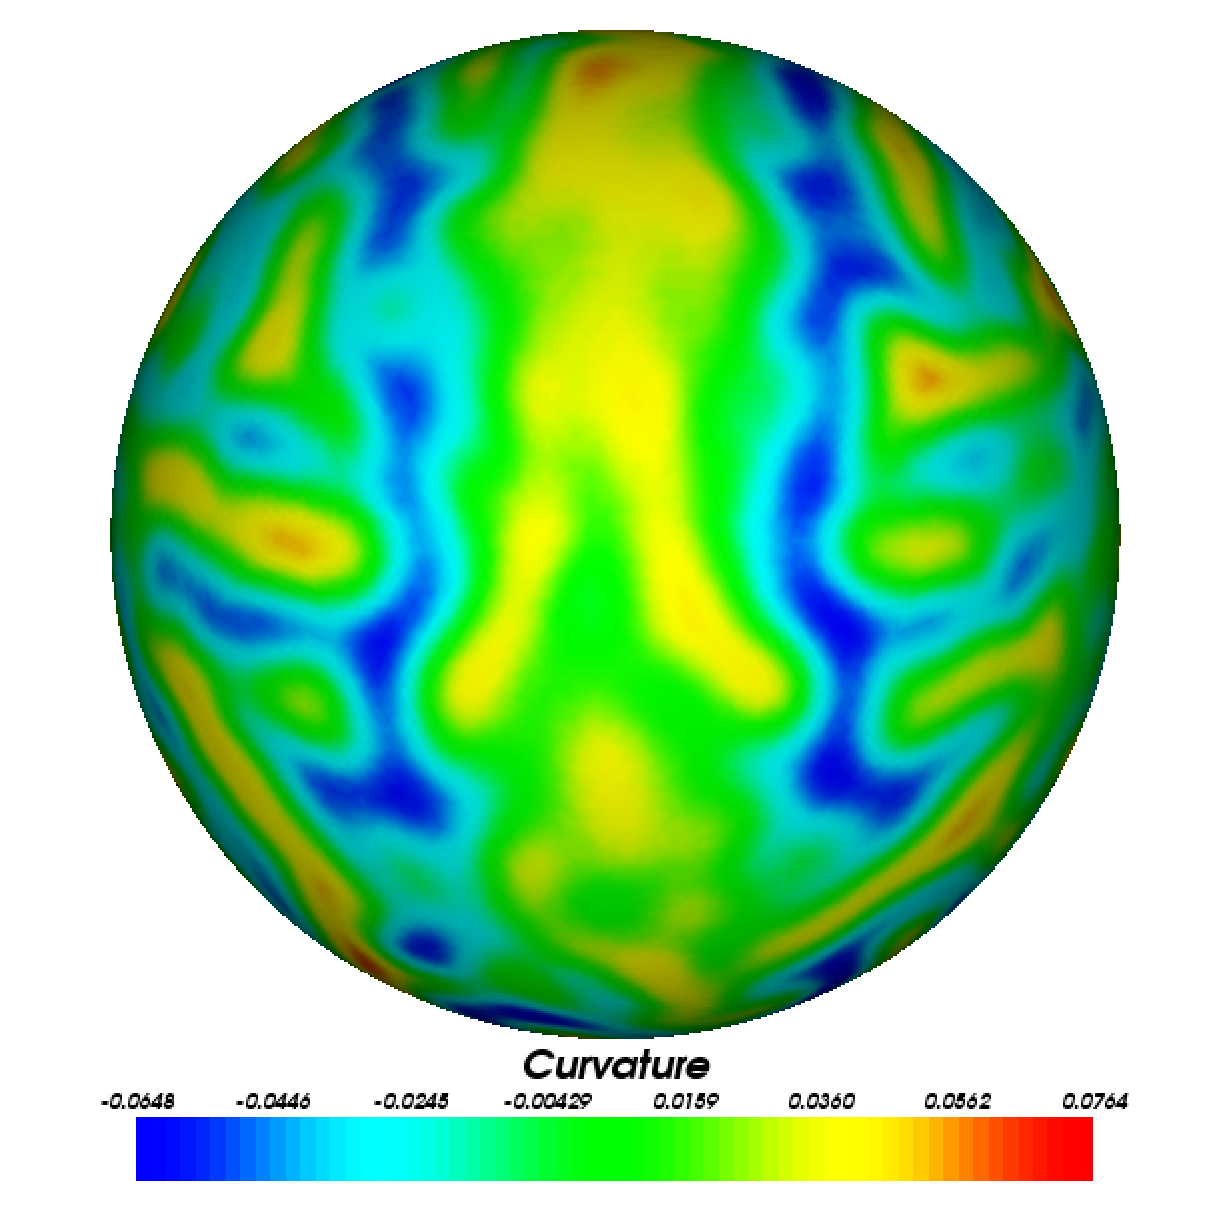
\includegraphics[%
  width=0.5\linewidth,
  keepaspectratio]{00111_smooth_128.ps}&
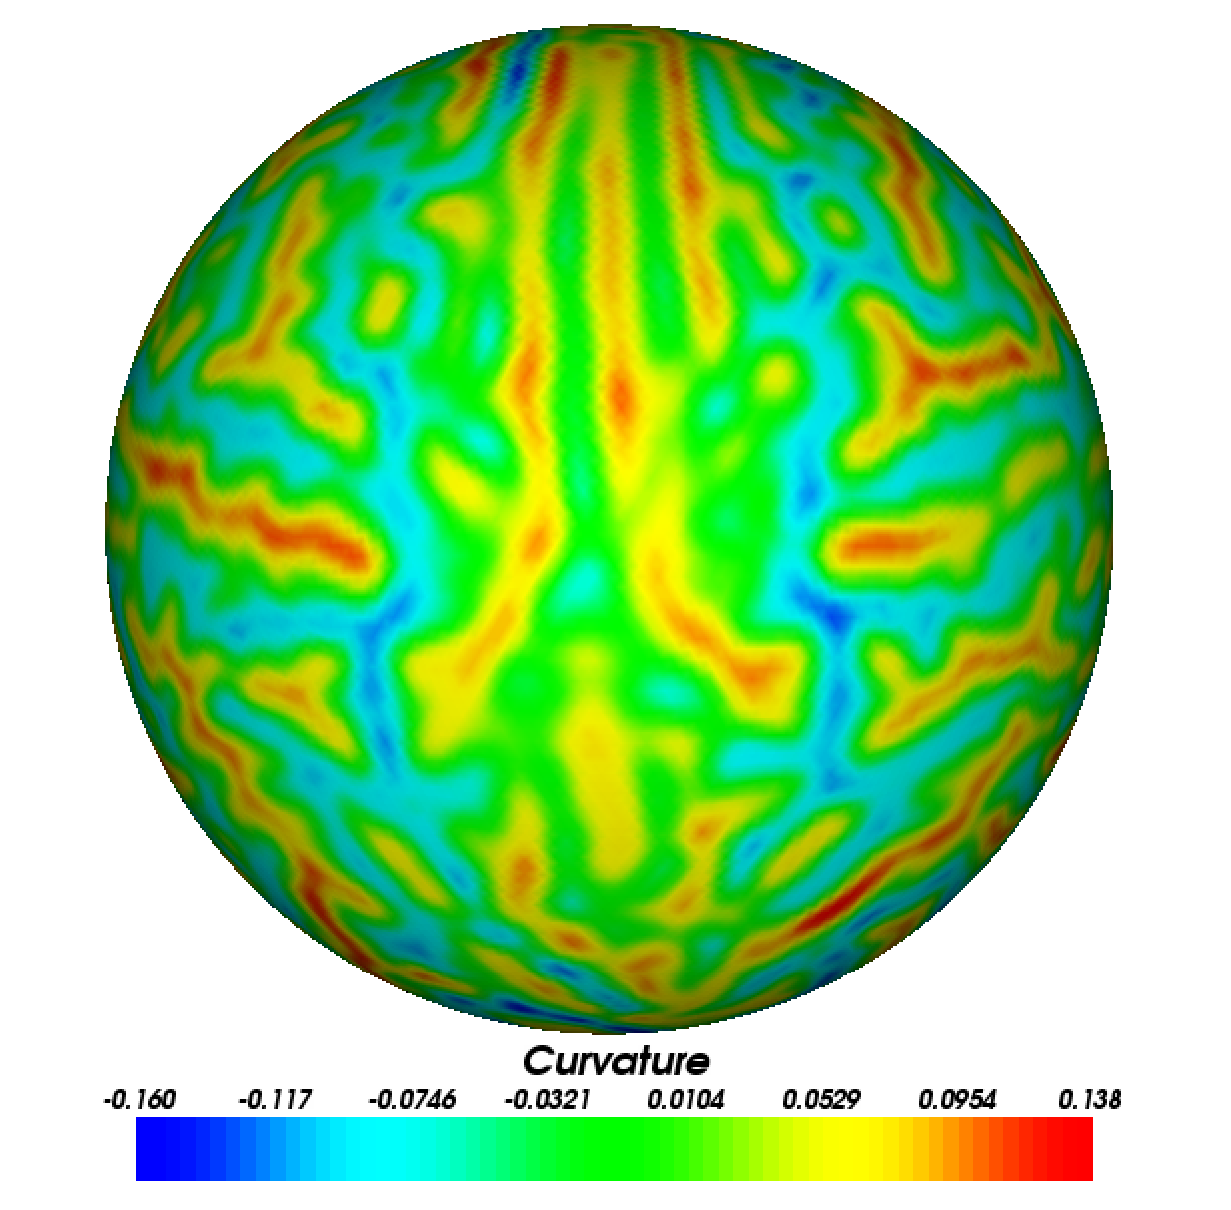
\includegraphics[%
  width=0.5\linewidth,
  keepaspectratio]{00111_smooth_32.ps}\tabularnewline
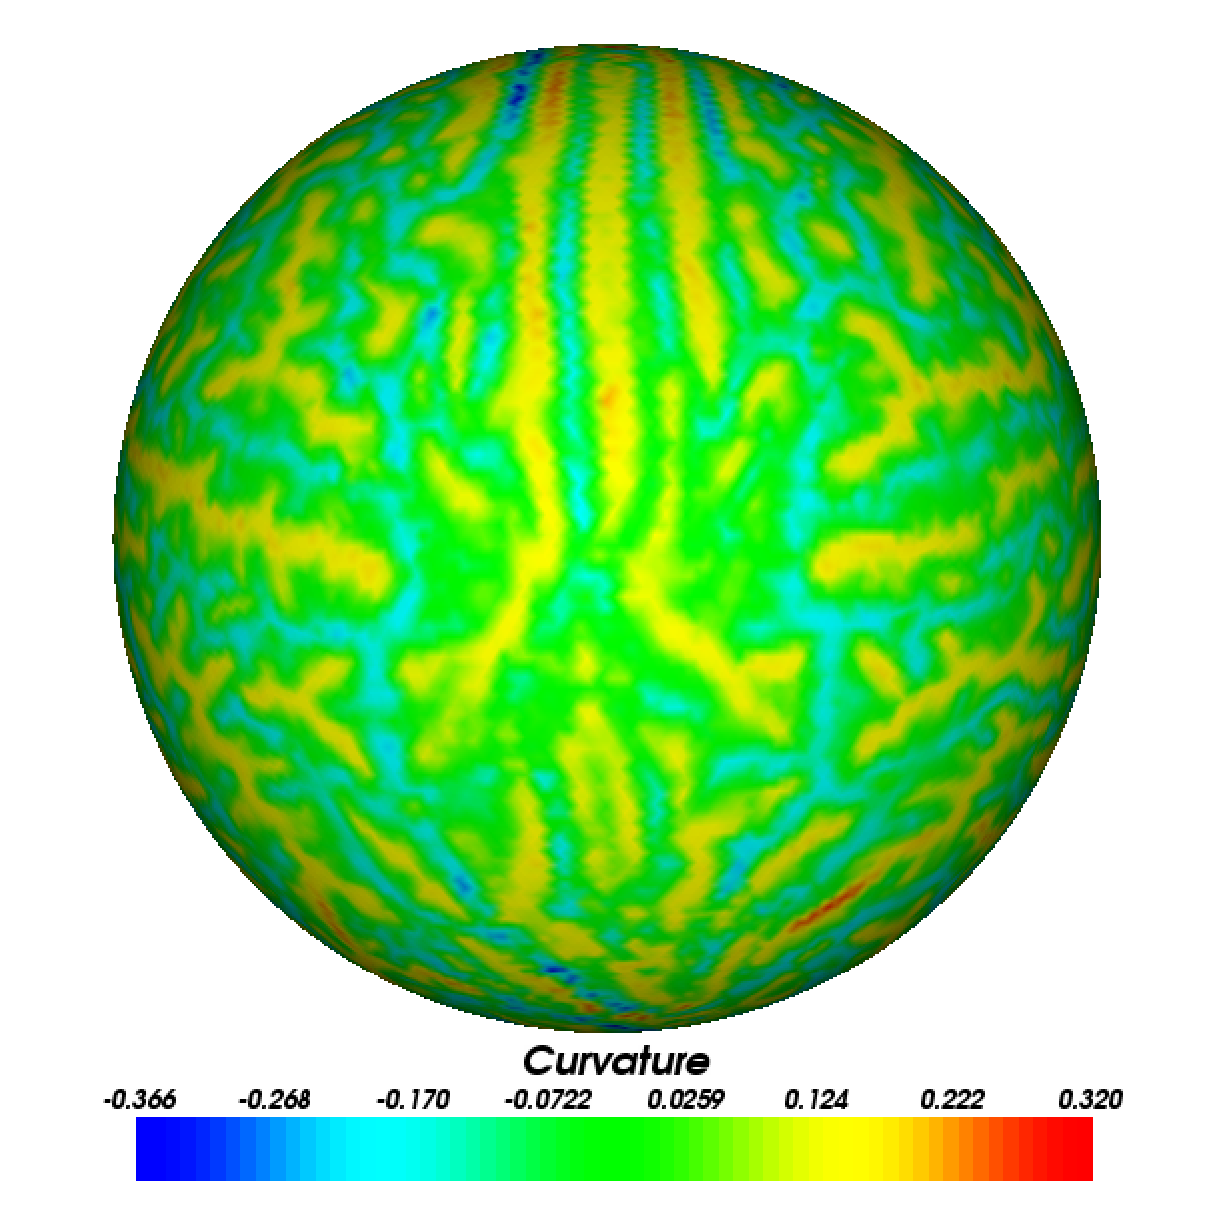
\includegraphics[%
  width=0.5\linewidth,
  keepaspectratio]{00111_smooth_8.ps}&
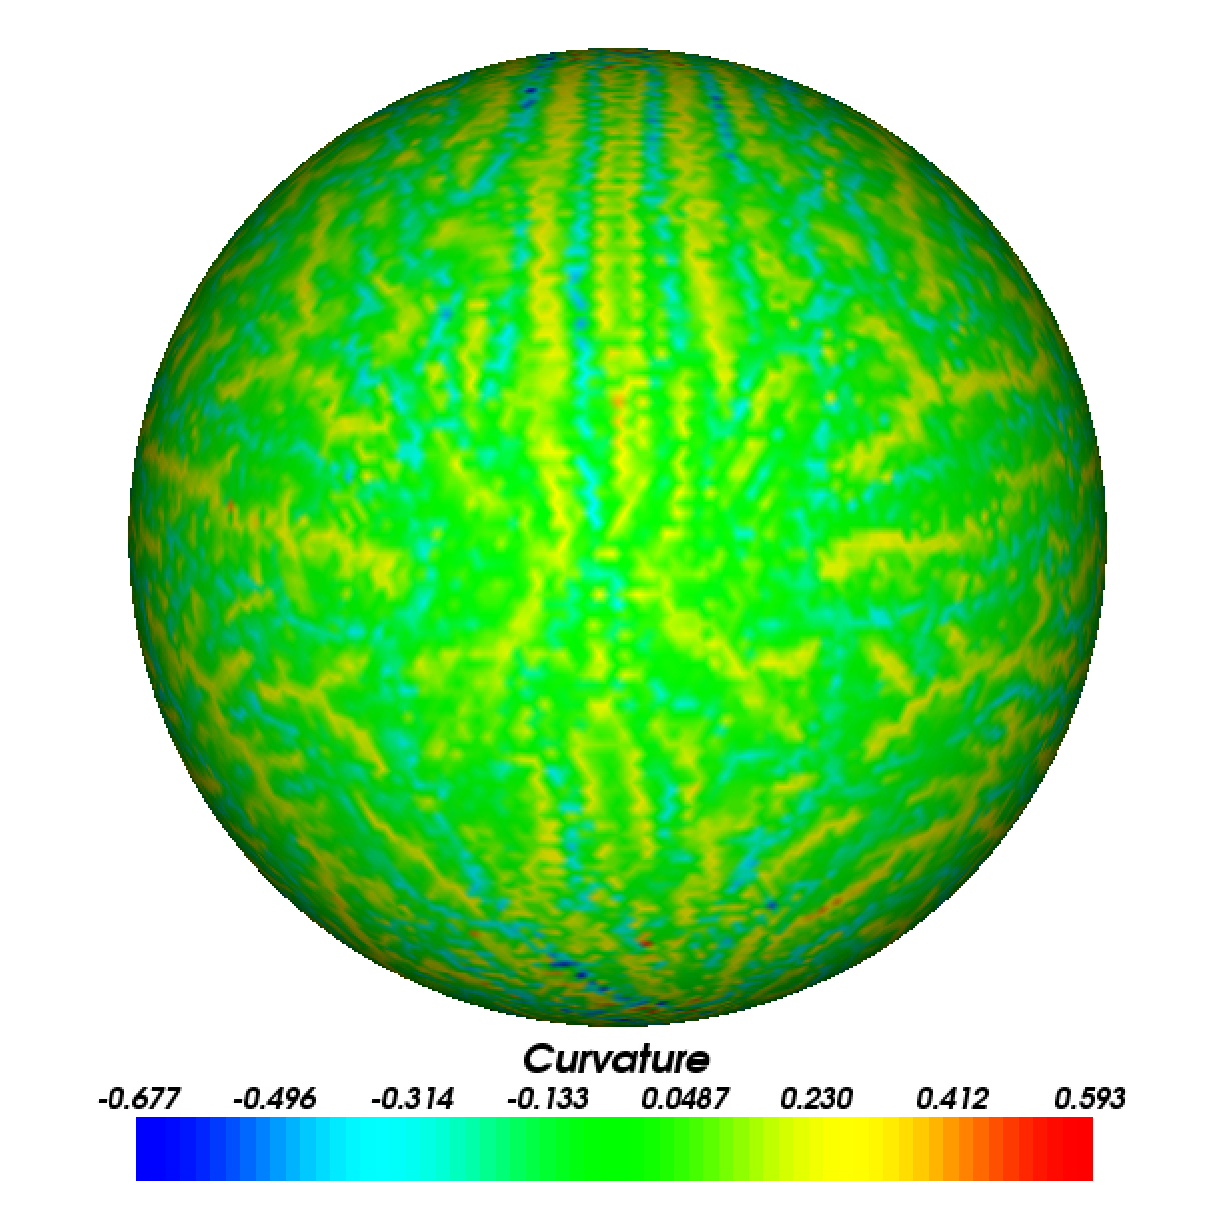
\includegraphics[%
  width=0.5\linewidth,
  keepaspectratio]{00111_smooth_2.ps}\tabularnewline
\end{tabular}\end{center}


\subsection{Inner Loop}

The optimization perfomed at each step of the coarse-to-fine outer
loop is the two-step Algorithm \ref{alg:Two-Step-Registration}, which
we call the inner loop.


\subsubsection{Matching (Step 2)}

The data term is written as a sum of terms, one for each vertex, $\Phi_{D}(U)=\sum_{v}\phi^{v}(U)$.
Each term is based on the correlation coefficient similarity measure
\cite{roche00:max-likelihood}, that produces a value in range $[-1,1]$
with better match indicated by larger score. Since \noun{surftracc}
operates as a minimization, we need to invert this\[
\phi^{v}(U)=1-\phi_{CC}^{v}(U),\]
where $\phi_{CC}^{v}$ is the correlation coefficient evaluated between
a neighbourhood of $v$ on the source data and a neighbourhood of
$U(v)$ on the target data. 

Each neighbourhood is a spherical cap at the given centre point $p$,
where $p$ is either $v$ or $U(v)$. The correlation coefficient
is evaluated by sampling on a set of sample points in each neighbourhood.
The sample points are arranged on a disc of radius $R_{n}$ parallel
to the tangent plane at $p$, as illustrated below. 

\begin{center}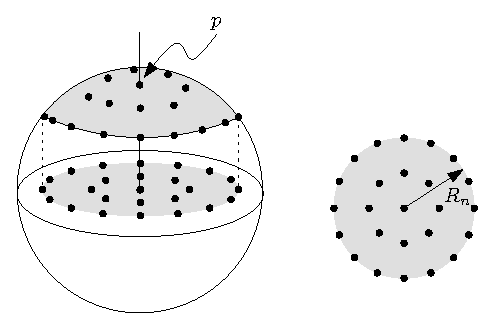
\includegraphics[%
  width=1\linewidth]{similarity-neighbourhood.eps}\end{center}

The set of sample points are: the centre of the disc, 8 points equally
spaced around a circle of radius $R_{n}/2$, and 16 points equally
spaced on a circle of radius $R_{n}$. The disc radius is \begin{equation}
R_{n}=r_{n}d_{C},\label{eq:define-neighbourhood-radius}\end{equation}
 where $r_{n}$ is a user-specified radius factor, and $d_{C}$ sets
the distance scale based on the coarseness of the control mesh. The
value of $d_{C}$ is the distance, projected to the disc, from the
centre of the cap to a neighbouring control mesh vertex. In other
words, $d_{C}$ is the length of a typical control mesh edge after
projecting to the disc. The value of $R_{n}$ must be no greater than
1, so $r_{n}\le1/d_{C}$.

The penalty $\Psi$ is also written as a sum over nodes of the control
mesh, $\Psi(T-U)=a\sum_{v}\psi(||T(v)-U(v)||)$. The penalty function
$\psi$ is designed so that $U(v)$ is restricted to the hemisphere
centred on $T(v)$. This is easily done by choosing $\psi$ such that
it becomes infinite when the angle between $T(v)$ and $U(v)$ reaches
$\pi/2$. 

With the search space restricted to a hemisphere, it can be parameterized
using two variables, by projecting the points on the sphere to the
tangent plane at $T(v)$. Thus, $U(v)$ is obtained using a two-dimensional
unconstrained optimization. Points $T(v)$ and $U(v)$ are projected
to this disc and $r$ is defined as the distance between the projected
points as illustrated.

\begin{center}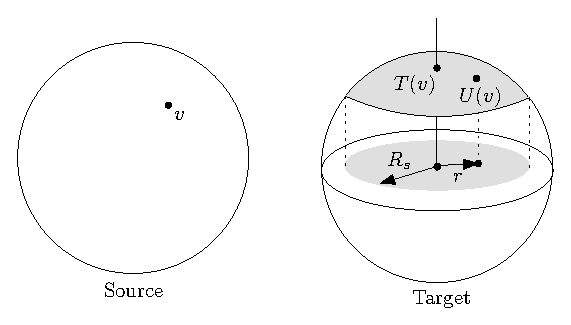
\includegraphics[%
  width=1\linewidth]{search-neighbourhood.eps}\end{center}

The penalty is a logarithmic barrier function \cite{nocedal99:numerical-optimization},
$\psi=-\log(1-r^{2}/R_{s}^{2})$, which has the effect of constraining
the search for $U(v)$ to points with $r<R_{s}$. The disc radius
is \begin{equation}
R_{s}=r_{s}d_{T},\label{eq:define-search-radius}\end{equation}
 where $r_{s}$ is a user-specified search radius factor, and $d_{T}$
sets the distance scale based on the control mesh. The value of $d_{T}$
is the distance, projected to the disc, between $T(v)$ and $T(u)$
where $u$ is the control-mesh neighbour closest to $v$ on the target,
i.e. $||T(v)-T(u)||$ is minimum for all 1-ring neighbours $u$ of
$v$. The value of $R_{s}$ must be no greater than 1, so $r_{s}\le1/d_{T}$.

The objective function is designed to be separable so that the minimization
of \begin{equation}
\phi^{v}(U(v))+a\psi(||U(v)-T(v)||)\label{eq:objective-vertex-v-2d}\end{equation}
 is performed independently for each control mesh vertex $v$. Each
optimization is a 2-dimensional problem, parameterized by Cartesian
coordinates in the tangent plane at $T(v)$. The initial iterate is
$(0,0)$ which corresponds to $T(v)$, and is a feasible point since
it corresponds to $r=0$ so the barrier function $\psi$ is zero.
The optimization is performed using the Nelder-Mead downhill simplex
algorithm \cite{press88:numerical-recipes} as implemented in the
GNU Scientific Library \cite{galassi02:gsl-book}. The Nelder-Mead
simplex algorithm is chosen because it does not require derivatives
of the objective function \ref{eq:objective-vertex-v-2d}, which are
complicated due to the correlation coefficient data term in $\phi^{v}$. 


\subsubsection{Smoothing (Step 3)}

The smoothing, which is carried out in $\Rthree$, is a simple weighted
average of $U(v)$ and the centroid of its neighbourhood, \[
C(v)=\frac{1}{|N_{v}|}\sum_{u\in N_{v}}U(u),\]
where $N_{v}$ is the set of neighbours of $v$. The smoothed transformation
is given by \[
T(v)=\frac{U(v)+wC(v)}{||U(v)+wC(v)||},\]
where $w$ is a user-specified smoothing weight.


\subsection{Algorithm Parameters}

The user of this algorithm has four major parameters to specify: the
search radius $r_{s}$, the neighbourhood radius $r_{n}$, the penalty
ratio $a$, and the smoothing weight $w$. Note that the search radius
and neighbourhood radius are dimensionless quantities that multiply
a length set by the coarseness of the control mesh through Equations
\ref{eq:define-neighbourhood-radius} and \ref{eq:define-search-radius},
respectively. Thus $r_{s}$ and $r_{n}$ can be set to a fixed value
for all iterations of the outer coarse-to-fine loop, as are parameters
$a$ and $w$.


\section{Output}

The output is a map $T:\Stwo\rightarrow\Stwo$, specified in a piecewise
linear fashion by providing $T(v)$ for all vertices $v$ of the control
mesh. The transformation at vertex $v$ is a point $T(v)\in\Stwo$.
However, instead of storing the Euclidean coordinates for the point
$T(v)$, the triple $(h,\alpha,\beta)$ is stored where $h$ is a
halfedge (internally represented as a pointer) specifying the spherical
triangle of the target data mesh that contains $T(v)$ and $(\alpha,\beta)$
are the areal coordinates (along with $\gamma\equiv1-\alpha-\beta$)
locating $T(v)$ on the spherical triangle as illustrated.

\begin{center}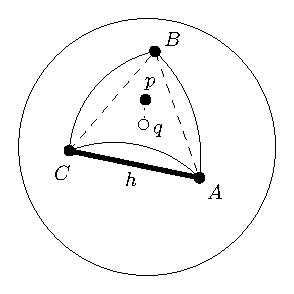
\includegraphics{surfacepoint.eps}\end{center}

%% LyX 1.3 created this file.  For more info, see http://www.lyx.org/.
%% Do not edit unless you really know what you are doing.
\documentclass[10pt,letterpaper,twocolumn,english]{article}
\usepackage{ae}
\usepackage{aecompl}
\usepackage[T1]{fontenc}
\usepackage[latin1]{inputenc}
\usepackage{float}
\usepackage{amsmath}
\usepackage{graphicx}
\usepackage{amssymb}

\makeatletter

%%%%%%%%%%%%%%%%%%%%%%%%%%%%%% LyX specific LaTeX commands.
\newcommand{\noun}[1]{\textsc{#1}}
%% Because html converters don't know tabularnewline
\providecommand{\tabularnewline}{\\}
\floatstyle{ruled}
\newfloat{algorithm}{tbp}{loa}
\floatname{algorithm}{Algorithm}

%%%%%%%%%%%%%%%%%%%%%%%%%%%%%% User specified LaTeX commands.
\usepackage{url}

\newcommand{\inlinedef}[1]{\emph{#1}\index{#1}\glossary{#1}}
\newcommand{\sphericaltri}{\textcircled{$\triangle$}}

\usepackage{babel}
\makeatother
\begin{document}

\title{The Theory and Practice of Non-Rigid Surface Warping}


\author{Steven M. Robbins}

\maketitle

\newcommand{\Real}{\mathbb{R}}

\newcommand{\Rthree}{\mathbb{R}^{3}}

\newcommand{\Stwo}{\mathbb{S}^{2}}



\section{Introduction}

Surface registration is a procedure that produces a spatial mapping
from one surface, which we call the \emph{source} surface, to a second,
\emph{target}, surface. This manual is not a treatise on surface registration
(see, e.g. \cite{robbins03:phd}) but only documents the specific
theory and practice underlying \noun{surftracc}. 


\section{Input Data}

The input to surface registration is a pair of surfaces such as those
generated from a 3D MR image using software such as \noun{asp}/\noun{clasp}\cite{macdonald00:cortical-surfaces}.
In adition, a feature data function for each surface is required.


\subsection{Surface Description}

Each input surface must be a triangulated polyhedral surface, also
called a \emph{mesh}. Further, \noun{surftracc} assumes that the
surface has a very specific structure as follows.

First of all, \noun{surftracc} requires that the mesh represent
a topological sphere, i.e. a closed surface that bounds a finite volume
of space.

A common way to refine a mesh is by quadrisection, in which each triangle
is replaced by four triangles by joining the midpoints of the three
edges, as shown.

\begin{center}\includegraphics{quadrisection.eps}\end{center}

In addition to being a topological sphere, \noun{surftracc} requires
that the mesh graph be a repeated quadrisection of an icosahedron,
the graph with 20 triangular faces and 12 vertices each of degree
five. Each quadrisection increases the number of faces by a factor
of four. The following table shows the number of faces and vertices
produced by repeated quadrisection.

\begin{center}\begin{tabular}{|c|c|c|}
\hline 
\# Quadrisections&
\# Faces&
\# Vertices\tabularnewline
\hline
\hline 
0&
20&
12\tabularnewline
\hline 
1&
80&
42\tabularnewline
\hline 
2&
320&
162\tabularnewline
\hline 
3&
1280&
642\tabularnewline
\hline 
4&
5120&
2562\tabularnewline
\hline 
5&
20480&
10242\tabularnewline
\hline 
6&
81920&
40962\tabularnewline
\hline 
7&
327680&
163842\tabularnewline
\hline
\end{tabular}\end{center}

Note that ASP/CLASP outputs surfaces of the form required by \noun{surftracc}.


\subsection{Match Feature}

Along with each surface, we need data to determine how the surfaces
match. The basic idea is to define a scalar \emph{feature} function
on each surface such that a matching region on the source and target
have a similar feature pattern. The feature values needn't match exactly
since, as described below, we use a correlation similarity measure
to drive the optimization.

The feature function is defined in a piecewise-linear fashion by providing
the function value at each vertex. At other points on the surface,
the function is interpolated from the 3 values at the triangle vertices.
This interpolation is described in more detail later.

We next describe two geometric feature functions that can be used
for registration: mean curvature and crown distance transform.


\subsubsection{Curvature}

The mean surface curvature is a popular choice for match feature since
gyral crowns and sulcal fundii have curvature of different sign. So
matching curvature should match gyrus to gyrus and sulcus to sulcus.

This Figure shows the value of mean curvature evaluated (using \cite{taubin95:estimating-curvature})
at each vertex of the cortical surface.

\begin{center}\begin{tabular}{cc}
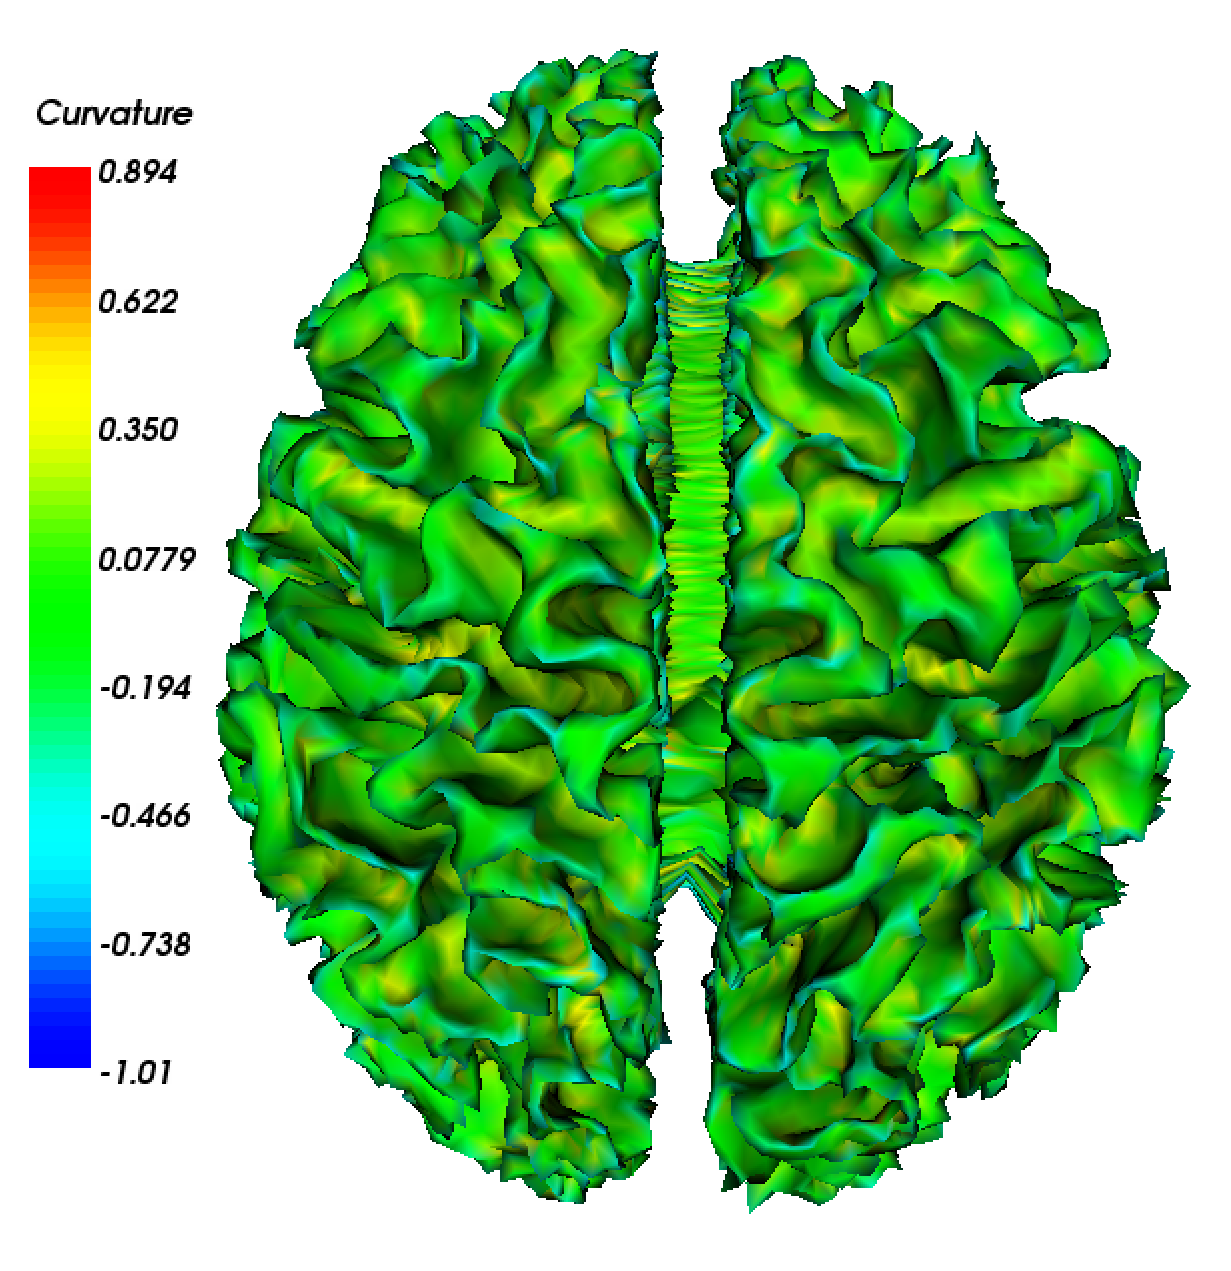
\includegraphics[%
  width=0.45\linewidth,
  keepaspectratio]{mean-cortex-top.ps}&
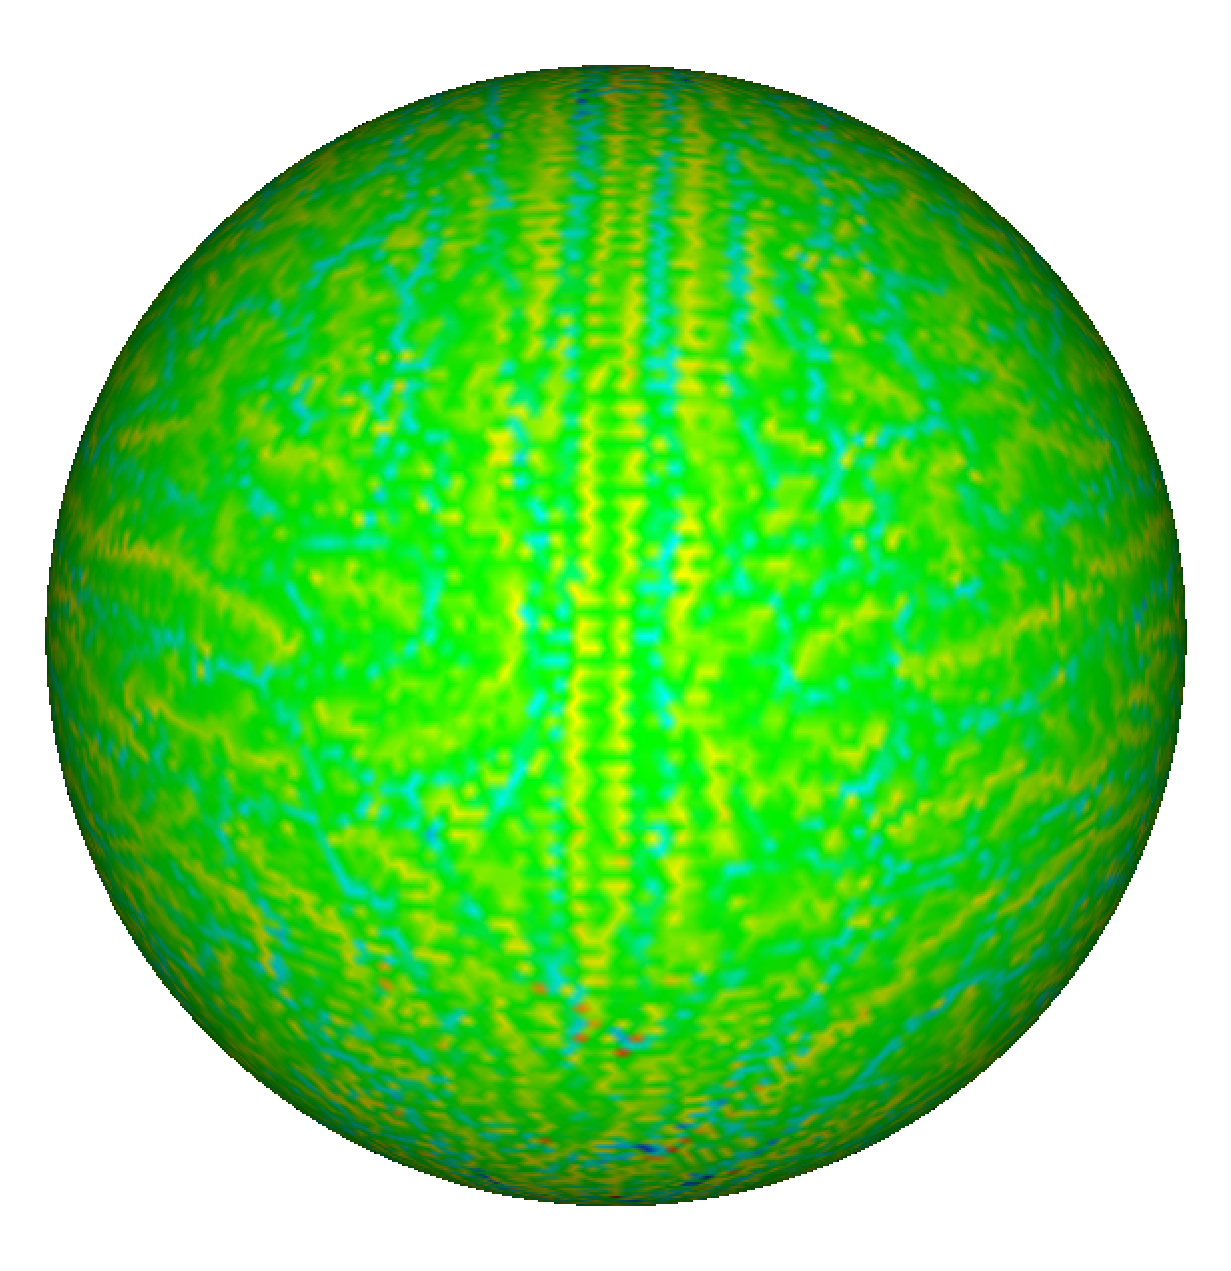
\includegraphics[%
  width=0.45\linewidth,
  keepaspectratio]{mean-sphere-top.ps}\tabularnewline
\end{tabular} \end{center}

Since sulcal fundi and gyral crowns have mean curvature of opposite
sign, registration based on matching mean curvature should tend to
match sulcus to sulcus and gyrus to gyrus. However, there is evidently
a lot of noise in the curvature map as well, due to small-scale oscillations
in the mesh vertex positions, so the data needs to be smoothed when
used for registration, either by smoothing the surface before computing
the curvature, or by directly averaging function values in a neighbourhood
of each vertex.


\subsubsection{Crown Distance Transform}

The intuition behind this feature, like that of mean curvature, is
that it is desirable to match points along the crown of a gyrus on
the source surface with points along the crown of a gyrus in the target
surface. Similarly, the fundus of a sulcus should match the fundus
of a sulcus. In contrast to matching by mean curvature, other points
on the bank of a sulcus are matched according to their fractional
distance towards the bottom of the sulcus, e.g. a vertex halfway down
the sulcus in the source mesh should match a point halfway down the
target sulcus.

Suppose vertex $v$ is located in a sulcus of the source mesh. Consider
two shortest geodesic paths, one from $v$ to the gyral crown and
the other from $v$ to the fundus. Let the length of the first of
these paths be $S(v)$ and let $S_{D}(v)$ be the sum of the two path
lengths. Distance $S_{D}(v)$ can be regarded as the depth of the
sulcus along a path through $v$. Let $R$ and $R_{D}$ be the analogous
distance functions for the target surface. The fractional depth of
vertex $v$ on the source mesh is $S(v)/S_{D}(v)$.

\begin{center}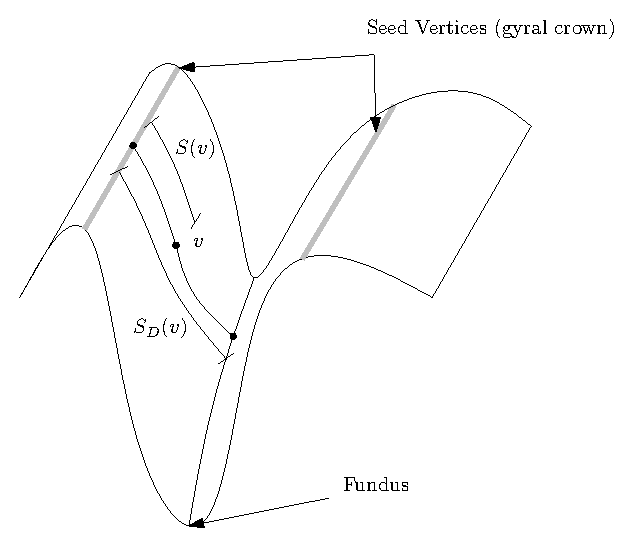
\includegraphics[%
  width=0.9\columnwidth,
  height=0.2\paperwidth,
  keepaspectratio]{fractional-depth.eps}\end{center}

The desired matching is to a point $T(v)$ on the target surface such
that $S(v)/S_{D}(v)\approx R(T(v))/R_{D}(T(v))$, or\begin{equation}
R(T(x))=\alpha(x)+\beta(x)S(x)+\epsilon(x),\label{eq:dt-matching-relation}\end{equation}
 where $\epsilon$ represents random noise, $\beta(x)=R_{D}(T(x))/S_{D}(x)$,
and $\alpha$ should be zero. However, $\alpha$ is left free to compensate
for practical difficulties in computing $S(x)$ and $R(x)$. Note
that points near to $v$ should have depth values close to $S_{D}(v)$
and similarly points near $T(v)$ should have depth values close to
$R_{D}(T(v))$. Assuming that $\alpha$ and $\beta$ are slowly-varying
functions, the maximum likelihood estimate for $T$ corresponds to
maximizing the regional correlation coefficient \cite{robbins03:phd}. 

Note that only the gyral crown distance functions, $S$ and $R$ appear
in Equation~\ref{eq:dt-matching-relation} and not $S_{D}$ and $R_{D}$.
Thus, the feature value stored at each vertex is the geodesic \emph{distance
transform} from a set of gyral {}``seed'' vertices, i.e. the length
of the shortest geodesic path from $v$ to a vertex in the seed set.


\paragraph{Seed Points}

The vertices chosen to be the seeds should in principle be all vertices
located on all the gyral crowns. We can identify gyral vertices with
the help of an \emph{$\alpha$-shape} \cite{edelsbrunner94:alpha-shapes},
a discrete geometry notion that can be considered as a relaxation
of the convex hull. The degree of relaxation is controlled by the
parameter $\alpha$ in the following manner. Let $S$ be a set of
points in $\Rthree$. Define an \emph{$\alpha$-ball}%
\footnote{The definition given here follows the Computational Geometry Algorithms
Library (CGAL) \cite{cgal-web}, as the implementation of $\alpha$-shape
provided by CGAL is used. In the original definition of Edelsbrunner
and M�cke, $\alpha$ is the radius of the $\alpha$-ball.%
} to be a closed ball of radius $\sqrt{\alpha}$, i.e. the point set
$\{ x\in\Rthree:||x-p||\le\sqrt{\alpha}\}$, for some $p\in\Rthree$.
The points of $S$ that form the vertices of the $\alpha$-shape of
$S$ are those that lie on the boundary of an $\alpha$-ball with
no point of $S$ on the interior of the $\alpha$-ball. Such vertices
are said to be \emph{$\alpha$-exposed.} Note that convex hull vertices
are always $\alpha$-exposed, since for every point $x$ on the boundary
of a convex set, there exists a ball of radius $\sqrt{\alpha}$ for
any value of $\alpha$ that intersects the convex set only at $x$.
Thus the vertices of the $\alpha$-shape with $\alpha=\infty$ are
the vertices of the convex hull. As $\alpha$ is decreased, more points
become $\alpha$-exposed until at $\alpha=0$ all points are $\alpha$-exposed. 

Using $\alpha$-balls of radius 10 mm (i.e. $\alpha=100$), a value
empirically chosen using visual inspection of the results, produces
good outlines of several major gyri. However, there are also vertices
in the point set lying underneath the brain on the arbitrary {}``cap''
through the brain stem which should not form part of the seed set;
these vertices are masked out as follows. The distance transform is
computed using the convex hull points as the seed vertices and any
vertex with a distance transform value greater than 35 (a value chosen
empirically) is removed from the set of vertices of the $\alpha$-shape.
The remaining vertices form the seed set used for the crown distance
transform feature.


\paragraph{Geodesic Distance}

The distance transform used in practice is an approximation to the
geodesic distance, as computing true geodesic distance is computationally
costly and difficult to code robustly \cite{lanthier01:approx-weighted-shortest-path}.
The approximation is computed using the mesh graph with the weight
for each edge set to the Euclidean length of the edge. An additional
vertex, $s$, is inserted and attached to each seed vertex with a
zero weight edge. Then Dijkstra's single-source shortest path algorithm
\cite{cormen90:intro-algorithms} is run with $s$ as the source vertex.
To improve the accuracy of the approximation the mesh is refined before
running Dijkstra's shortest path algorithm. First, $m$ equally-space
extra points are inserted on each edge, then a new edge is inserted
for each pair of extra points that either (i) are adjacent on an original
edge, or (ii) are on different edges both of which are incident to
a common (original) facet. The approximate shortest path computed
by this algorithm consists of line segments which are either an edge
of the original surface, or cross a facet of the original surface
as shown.

\begin{center}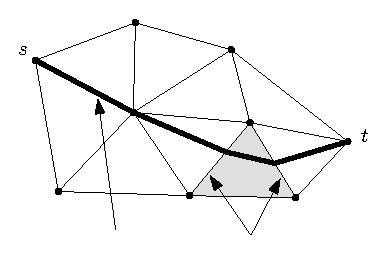
\includegraphics{approximate-path.eps}\end{center}

The crown distance transform from the final seed set is illustrated
below.

\begin{center}\begin{tabular}{cc}
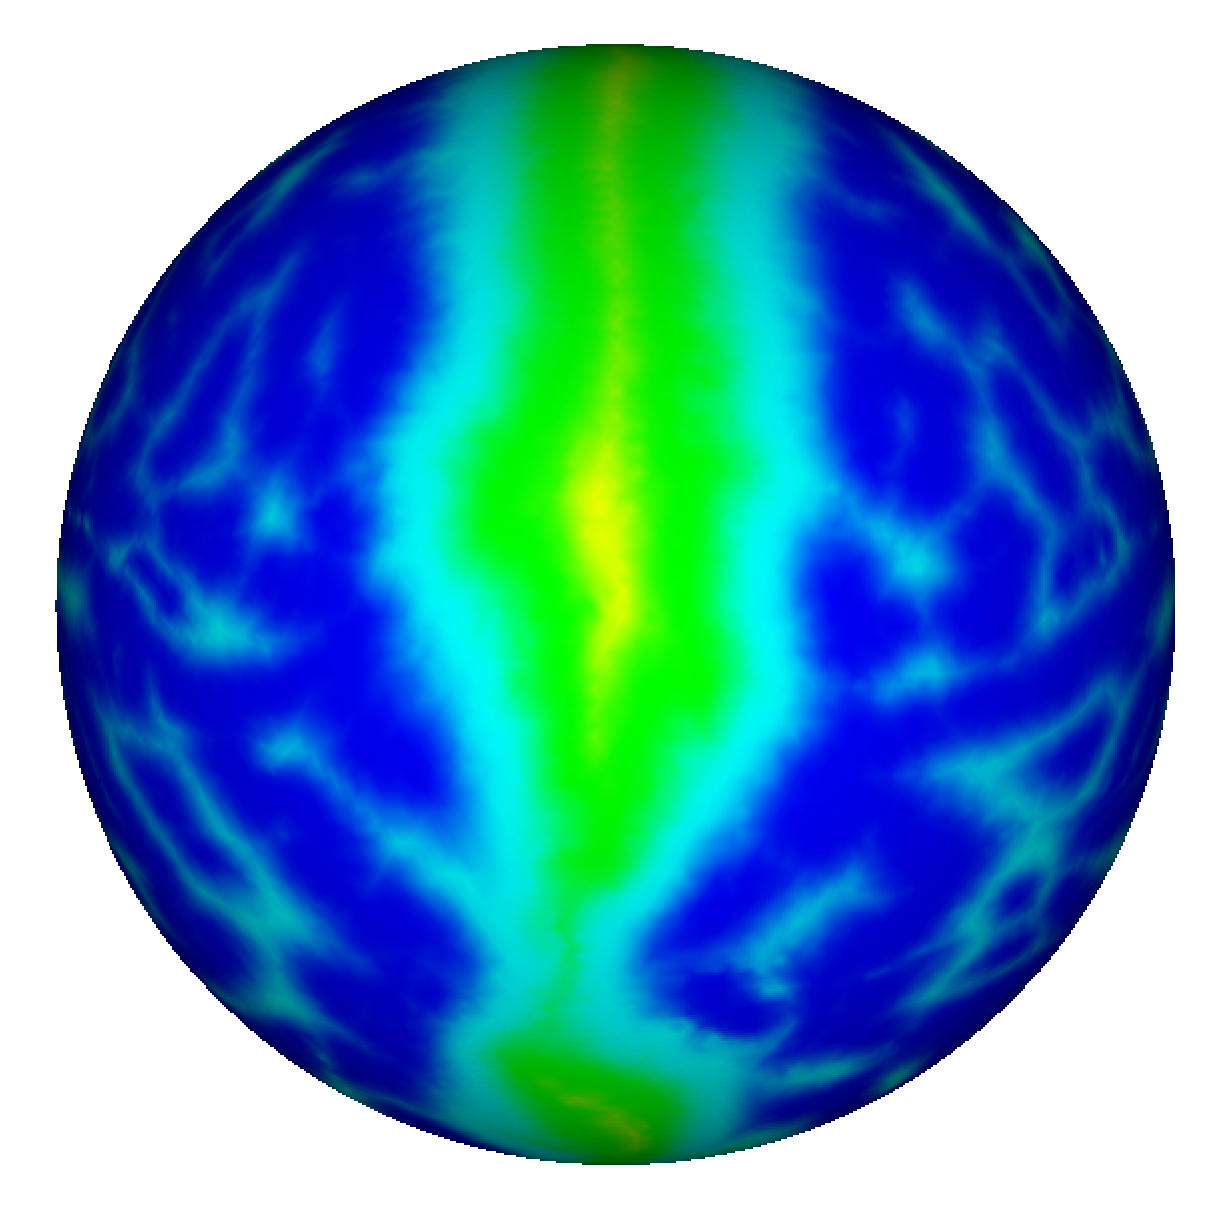
\includegraphics[%
  width=0.4\columnwidth,
  height=0.15\paperwidth,
  keepaspectratio]{sphere-top.ps}&
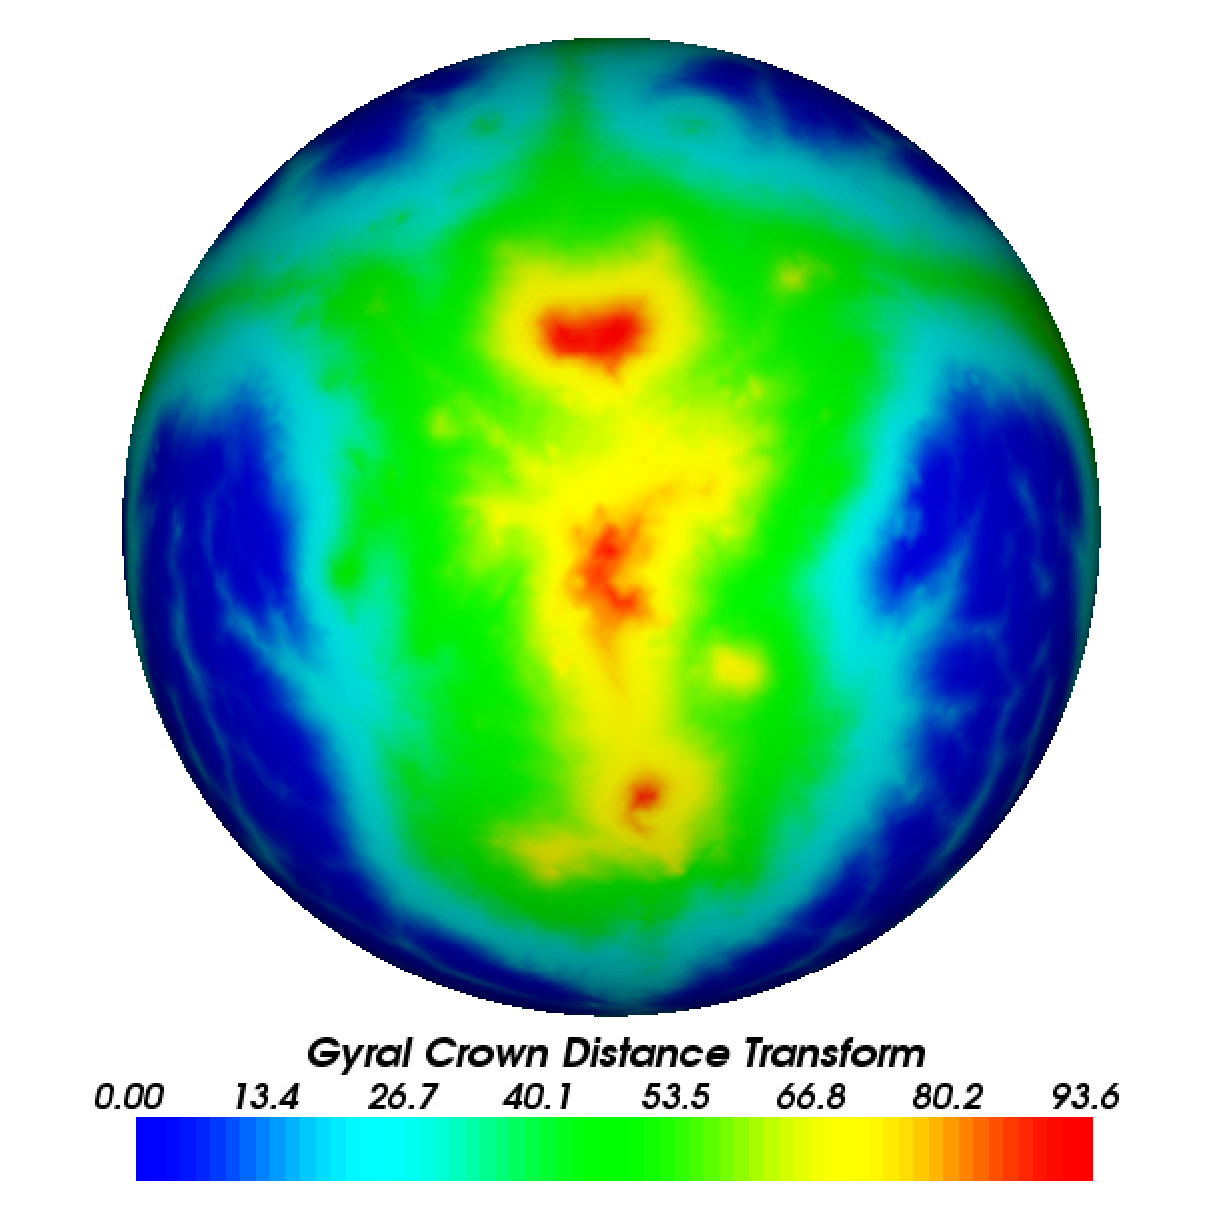
\includegraphics[%
  width=0.4\columnwidth,
  height=0.15\paperwidth,
  keepaspectratio]{sphere-bottom.ps}\tabularnewline
Top&
Bottom\tabularnewline
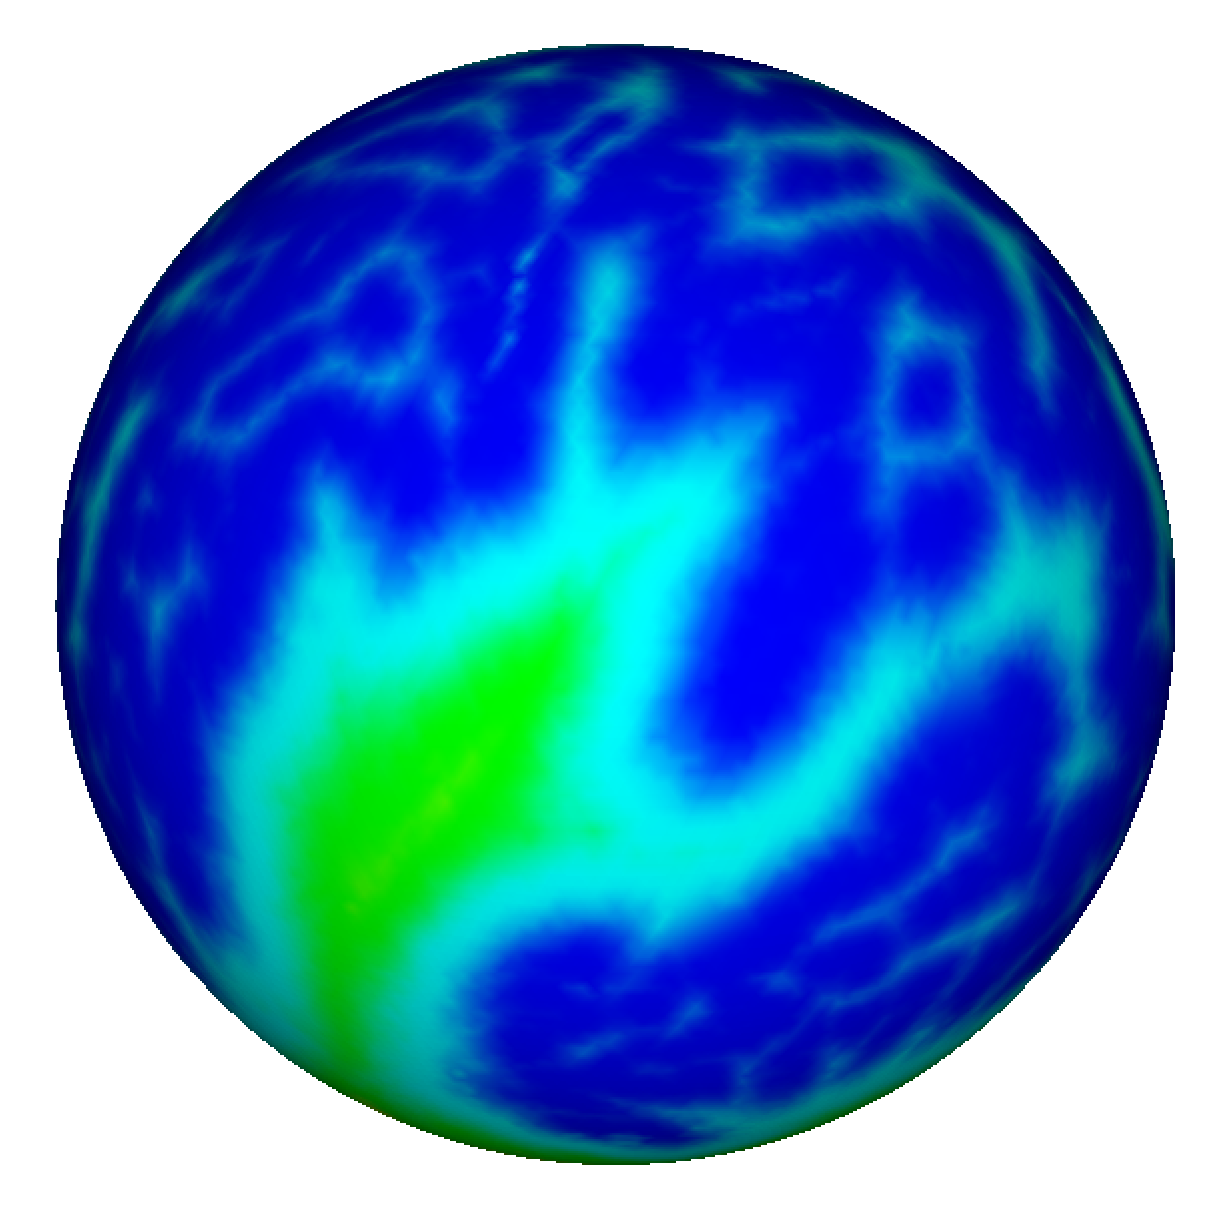
\includegraphics[%
  width=0.4\columnwidth,
  height=0.15\paperwidth,
  keepaspectratio]{sphere-left.ps}&
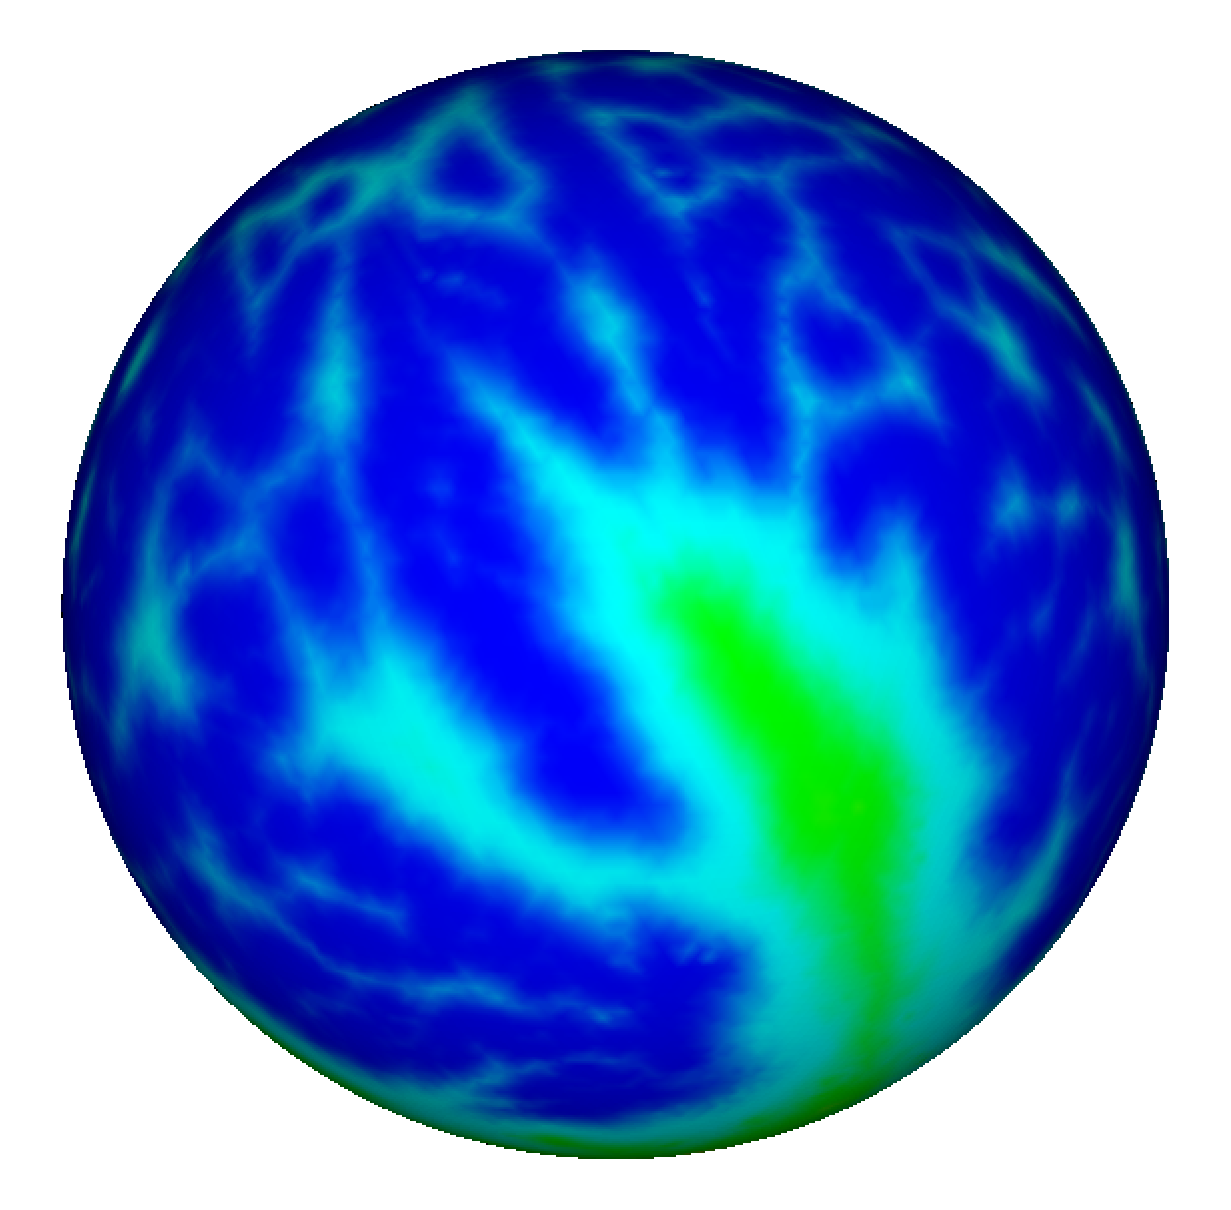
\includegraphics[%
  width=0.4\columnwidth,
  height=0.15\paperwidth,
  keepaspectratio]{sphere-right.ps}\tabularnewline
Left&
Right\tabularnewline
\end{tabular}\end{center}


\section{Triangle Interpolation}

Both the feature data function described above and, ultimately, the
transformation $T$ are defined at mesh vertices and interpolated
across the rest of the surface. We pause to discuss this interpolation
before discussing the optimization used to search for $T$.


\subsection{Scalar Function Interpolation}

Suppose that for a function, $f$, a real value is associated with
each vertex of the mesh, as is the case for the feature function data.
Let $p$ be a point on the mesh and consider what value to assign
$f(p)$. 

If $p$ is a vertex, the vertex value is assigned. 

If $p$ is not a vertex, let $ABC$ be a triangle of the mesh that
contains $p$. There is a unique triple of real values $(\alpha,\beta,\gamma)$
with $\alpha+\beta+\gamma=1$ that satisfies $p=\alpha A+\beta B+\gamma C$.
This triple is known as the \emph{areal coordinates} of $p$ \cite[section 13.7]{coxeter69:intro-geometry}.
We use these values for interpolation, assigning $f(p)=\alpha f(A)+\beta f(B)+\gamma f(C)$.
It is clear that this choice of interpolation (a) is consistent with
the assigned values at vertices $A$, $B$, and $C$, and (b) gives
consistent values along a shared triangle edge no matter which triangle
is used for the interpolation.


\subsection{Triangulation Warping}


\subsubsection{Auxiliary Space}

While it is conceivable to define the mapping $T$ directly on the
input mesh, it is easier to use a simpler auxiliary space instead;
\noun{surftracc} uses the unit sphere. The source mesh, $M_{I}$,
is first mapped to the sphere using an invertible projection map,
$\Pi_{I}$. This projection is given implicitly by the fact that $M_{I}$
is constrained to be a repeated quadrisection of the icosahedron,
as discussed above. The target surface $M_{J}$ is similarly projected
to the sphere by $\Pi_{J}$. The registration algorithm then computes
$T:\Stwo\rightarrow\Stwo$ which, together with the two projection
operations, serves to define map between the two input surface meshes,
denoted $W:M_{I}\rightarrow M_{J}$ in the diagram.

\begin{center}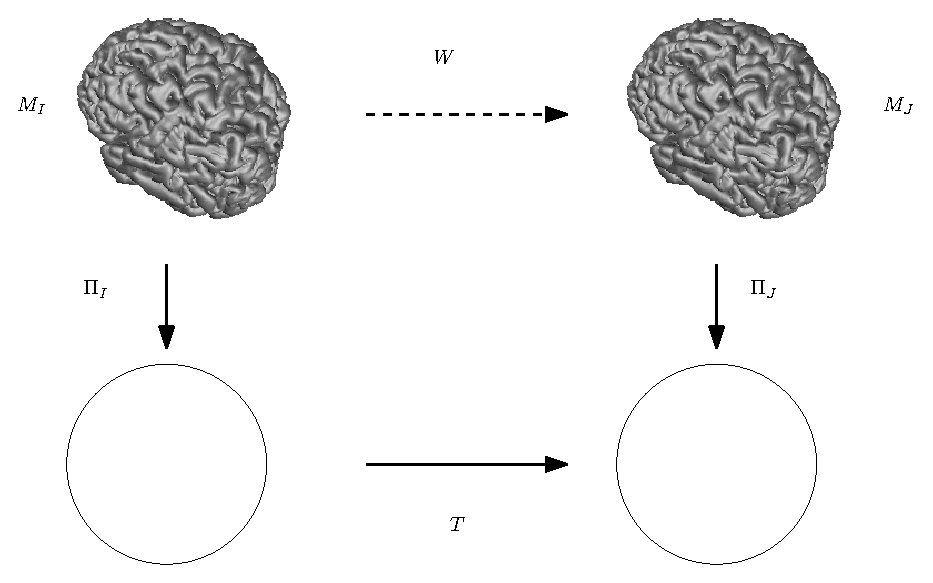
\includegraphics[%
  width=1\columnwidth,
  keepaspectratio]{mappings.eps}\end{center}


\subsubsection{Triangulation Warping on the Sphere}

We discuss now how the sphere-to-sphere mapping, $T:\Stwo\rightarrow\Stwo$
is defined. The basic idea is that the source sphere is partitioned
into spherical triangles, and the mapping under $T$ is given for
each spherical triangle. 


\paragraph{Mapping one Triangle}

Let $A$, $B$, and $C$ be three points on the sphere $\Stwo$ that
are not coplanar with the origin. Using projection from the origin,
i.e. the mapping $x\mapsto x/||x||$, the planar triangle $ABC$ is
put into 1-1 correspondence with a triangular patch of $\Stwo$ bounded
by three shortest geodesics, from $A$ to $B$, from $B$ to $C$,
and from $C$ to $A$. Each geodesic bounding the patch is denoted
an \emph{edge arc}, and the triangular patch of $\Stwo$ is known
as the \emph{spherical triangle} $\sphericaltri ABC$. Given the 1-1
mapping between the planar triangle $\triangle ABC$ and the spherical
triangle $\sphericaltri ABC$, areal coordinates can be used to refer
to either $q=\alpha A+\beta B+\gamma C\in\triangle ABC$ or to $p=q/||q||\in\sphericaltri ABC$.

The mapping of $\sphericaltri ABC$ begins by specifying the positions
of the vertices under the mapping; define $A'\equiv T(A)$, $B'\equiv T(B)$,
and $C'\equiv T(C)$. Define a mapping from point $p$ in spherical
triangle $\sphericaltri ABC$ to point $T(p)$ in spherical triangle
$\sphericaltri A'B'C'$ as follows. First, project $p$ to point $q$
on the planar triangle $ABC$ and compute the areal coordinates of
$q$. We define the corresponding point $q'\in\triangle A'B'C'$ using
$q'\equiv\alpha A'+\beta B'+\gamma C'$. Finally, $q'$ is projected
to point on the sphere, denoted $p'$ and we define $T(p)$ to be
$p'$. 

\begin{center}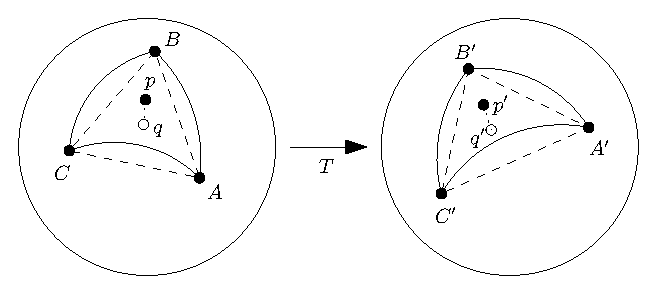
\includegraphics[%
  width=1\columnwidth,
  keepaspectratio]{trianglemap-sphere.eps}\end{center}


\paragraph{Mapping the Entire Sphere}

In order to map the entire sphere, all we need is a partitioning of
the sphere into a set of non-overlapping spherical triangles. For
each triangle, we use the procedure just described to map it. Since
each point of the input sphere is contained in at least one triangle,
a mapping of the sphere is achieved. As is the case when interpolating
real values, the interpolation of $T$ is consistent at vertices and
along edges of each spherical triangle. The overall mapping $T$ is
1-1 and invertible if it satisfies certain conditions \cite{robbins03:phd}.
The main two conditions are that (a) the orientation of each spherical
triangle is preserved (i.e. the triangle is not {}``flipped'') and
(b) for each vertex, the cyclic ordering of its neighbouring vertices
is preserved.

Note that the partitioning of the source sphere is equivalent to finding
a simple triangulated mesh, denoted the \emph{control} mesh, inscribed
in the sphere. The input meshes to \noun{surftracc} provide such
a mesh due to the constraint that they be obtained by repeated quadrisection
of the icosahedron.


\section{Optimizing the Spatial Transformation}

Registration is generally cast in terms of an optimization problem,
in which we seek $T$ that will optimize the match of the feature
function defined on each surface. \noun{surftracc} uses a minimization
with a correlation coefficient-based objective function that penalizes
difference between the feature value at corresponding points on the
surfaces.

In addition, the objective function incorporates a \emph{regularization}
term that penalizes a transformation that is unlikely. Let $S$ and
$R$ be the feature functions on the source and target surfaces, respectively.
The objective function $\Phi$ is expressed as a sum \begin{equation}
\Phi(S,R,T)=\Phi_{D}(S,R,T)+\Phi_{R}(T),\label{eq:obj-is-data-plus-reg}\end{equation}
 and the optimization problem to solve becomes 

\[
T=\arg\min_{T'}\Phi(S,R,T').\]
 

As discussed in the previous section, $T$ is given by specifying
its value at each vertex. The transformation value is a point on $\Stwo$,
which takes two parameters to specify (e.g. latitude and longitude),
so the registration algorithm has two parameters to optimize per vertex.
With so many parameters to estimate (80k on a 40k mesh), it is important
to choose an effective optimization technique. 


\subsection{Two Step Non-Rigid Warping Algorithm}

The complexity is handled by separating the problem into a number
of smaller optimizations \cite{nocedal99:numerical-optimization},
one per vertex. To make this happen, both the data and regularization
terms in Equation \ref{eq:obj-is-data-plus-reg} must be \emph{separable,}
i.e. expressible as a sum of simpler terms. The parameters being optimized
should be partitioned amongst the terms and each term should involve
just a few of the parameters being optimized.

The data term, after discretization to evaluate it on the mesh, is
naturally separable into one term per mesh vertex $v$, involving
only the two values required to specify $T(v)$.

The regularization term can also be made separable by transforming
the problem into two interleaved minimizations. We modify the problem
by introducing a second transformation, $U$. A third term is introduced
into the objective function to link the transformations, resulting
in 

\begin{equation}
\Phi(T,U)=\Phi_{D}(U)+\Psi(T-U)+\Phi_{R}(T),\label{eq:two-step-objective-3d}\end{equation}
where $\Psi$ penalizes difference between $T$ and $U$; we might
use $\Psi(T-U)=\int||T-U||^{2}$, for example. After minimizing over
both $T$ and $U$, the transformation $T$ is returned as the final
solution. In other words, the registration problem solved is\[
\arg\min_{T}\Phi'(T),\]
where \[
\Phi'(T)=\arg\min_{U}\Phi(T,U).\]


The new objective function, Equation \ref{eq:two-step-objective-3d},
has twice as many variables as the original objective function, $\Phi_{D}+\Phi_{R}$.
The registration algorithm proceeds in a sequence of {}``half iteration''
steps. One half iteration fixes the variables that define $T$ while
optimizing $U$ \begin{equation}
U=\arg\min_{U'}\Phi(T,U')=\arg\min_{U'}\Phi_{D}(U')+\Psi(T-U').\label{eq:two-step-U}\end{equation}
The next half iteration fixes the variables that define $U$ while
optimizing $T$\begin{equation}
T=\arg\min_{T'}\Phi(T',U)=\arg\min_{T'}\Psi(T'-U)+\Phi_{R}(T').\label{eq:two-step-T}\end{equation}
 The first step (Expression \ref{eq:two-step-U}) can be seen as finding
a transformation, $U$, that matches the data while remaining close
to the previous solution, $T$ by virtue of $\Psi$. The second step
(Expression \ref{eq:two-step-T}) can be seen as regularizing the
transformation $U$ to produce a smoother transformation $T$. This
is summarized in Algorithm \ref{alg:Two-Step-Registration}. %
\begin{algorithm}

\caption{\label{alg:Two-Step-Registration}Two-Step Registration.}

\begin{enumerate}
\item Set $T$ to initial estimate.
\item Minimize $\Phi_{D}(U)+\Psi(T-U)$, where the term $\Psi$ penalizes
deviation of $U$ from $T$.
\item Set $T$ to be the smoothed version of $U$.
\item Repeat steps 2-3 until done.
\end{enumerate}

\end{algorithm}
 One cost of broadening the criterion for the two steps is that the
resulting algorithm may no longer be interpretable as a minimization
problem. 

One of the advantages of this algorithm is that $\Psi$ can easily
be chosen to be separable so that, when $\Phi_{D}$ is also separable,
the optimization in step 2 is separable. Step 3, though not necessarily
separable, requires only linear time and space. So the overall algorithm
is tractable.


\subsection{Coarse-to-Fine Hierarchy}

Non-rigid registration of the sort implemented here is almost universally
performed with multiple {}``resolutions'' of the transformation.
\noun{surftracc} implements this idea by running Algorithm~\ref{alg:Two-Step-Registration}
on a coarse control mesh of 1280 triangles (a three-fold quadrisection
of the icosahedron). The control mesh is then refined using quadrisection,
the mapping function $T$ is interpolated onto the new control mesh,
and Algorithm~\ref{alg:Two-Step-Registration} is run again.

As previously discussed, the input surface mesh is a quadrisection
of the icosahedron, typically six-fold (81920 triangles). The control
mesh begins as a three-fold quadrisection of the \emph{same} icosahedron.
Thus, after a number of repeated refine and registration steps, the
control mesh will exactly coincide with the input surface mesh. The
registration terminates at this point with the value of $T$ specified
for each vertex of the input mesh.


\subsubsection{Initial Surface Mapping}

In principle, the initial mapping of the coarsest control mesh should
be obtained by a low-dimensional warping, e.g. searching for the optimal
rotation of the sphere. However, the current implementation of \noun{surftracc}
assumes the user has done this as a preprocessing step. Typically
this is achieved by obtaining both the source and target surfaces
using \noun{asp} from MR images that are initially registered using
a 9-parameter affine transformation to a common target. Since the
MR images are aligned, a given vertex $v$ of the initial mesh tends
to end up in a nearly homologous location on each image \cite{macdonald00:cortical-surfaces}.
This means that the initial transformation on the coarsest control
mesh can simply be set to the identity mapping. 


\subsubsection{Data Refinement}

When the feature value map requires smoothing so as to reduce noise,
the smoothing is typically done in a coarse-to-fine manner in step
with the control mesh refinement. The coarse control mesh is used
with heavily-smoothed data, with the amount of smoothing being reduced
after each level of the hierarchy.

One simple method for smoothing is as follows. Let $D(v)$ denote
the data value at vertex $v$. The data smoothing replaces, in parallel
for all $v$, $D(v)$ by \begin{equation}
(D(v)+a\sum_{u\in N_{v}}D(u))/\alpha,\label{eq:smooth-scalars}\end{equation}
where $N_{v}$ is the set of neighbours of $v$, $\alpha=1+a|N_{v}|$
is a scaling factor to ensure the weights add to 1, and $a$ is a
constant. The smoothing operation is iterated, say, 128 times at the
coarsest level of control mesh, 32 for the next, then 8, and finally
twice at the level of the finest control mesh. The result of such
smoothing the mean curvature data term shown below. 

\begin{center}\begin{tabular}{cc}
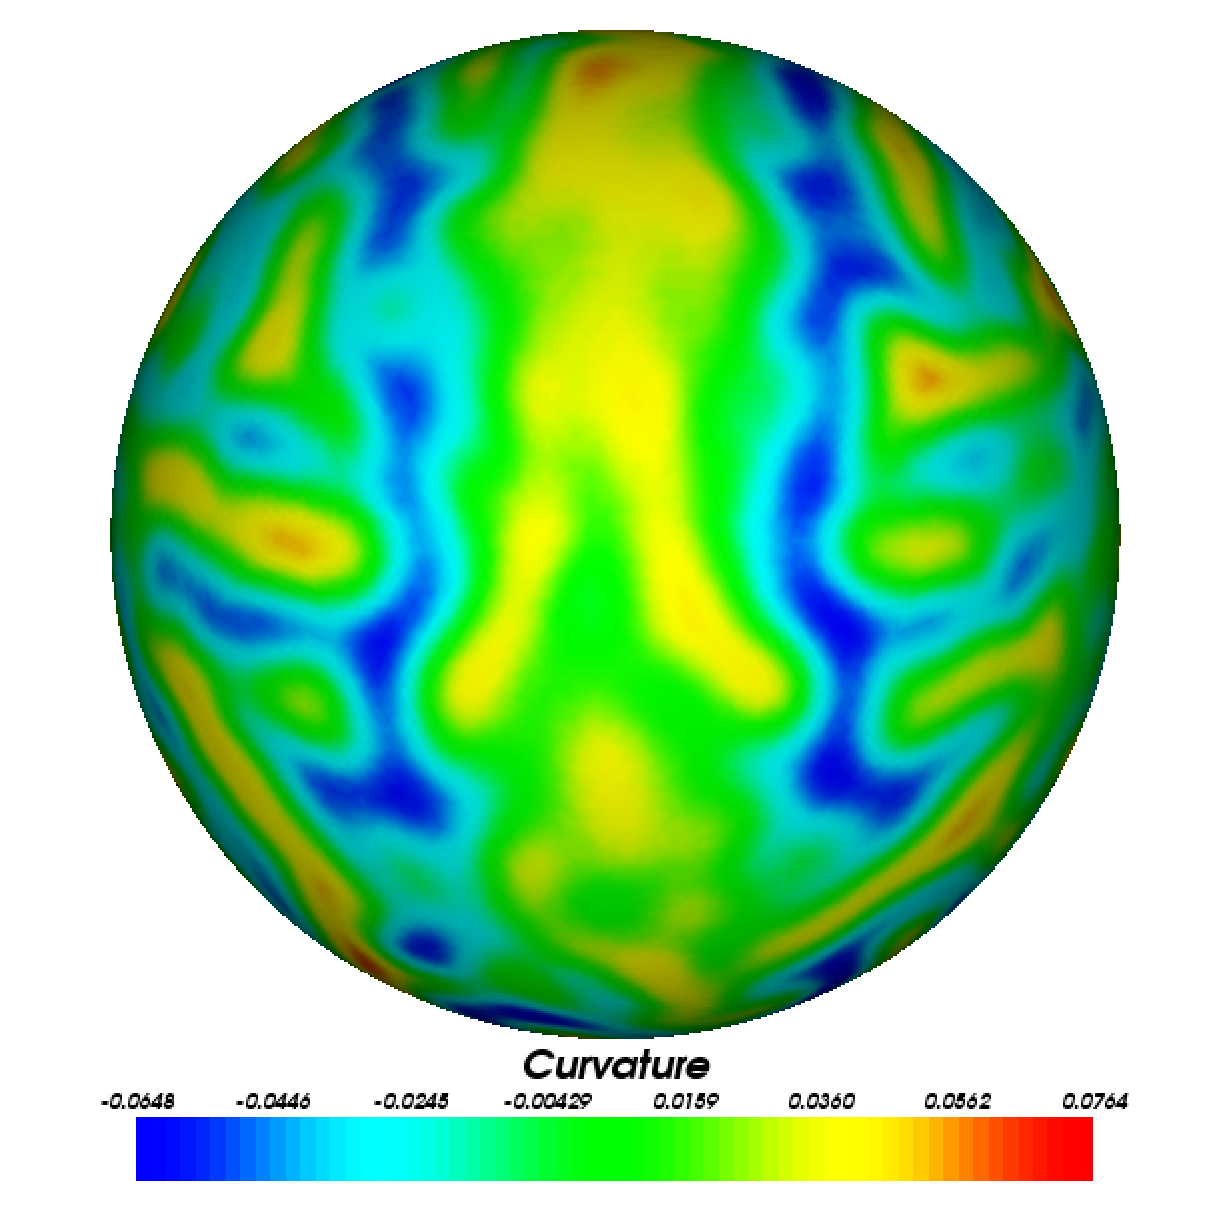
\includegraphics[%
  width=0.5\linewidth,
  keepaspectratio]{00111_smooth_128.ps}&
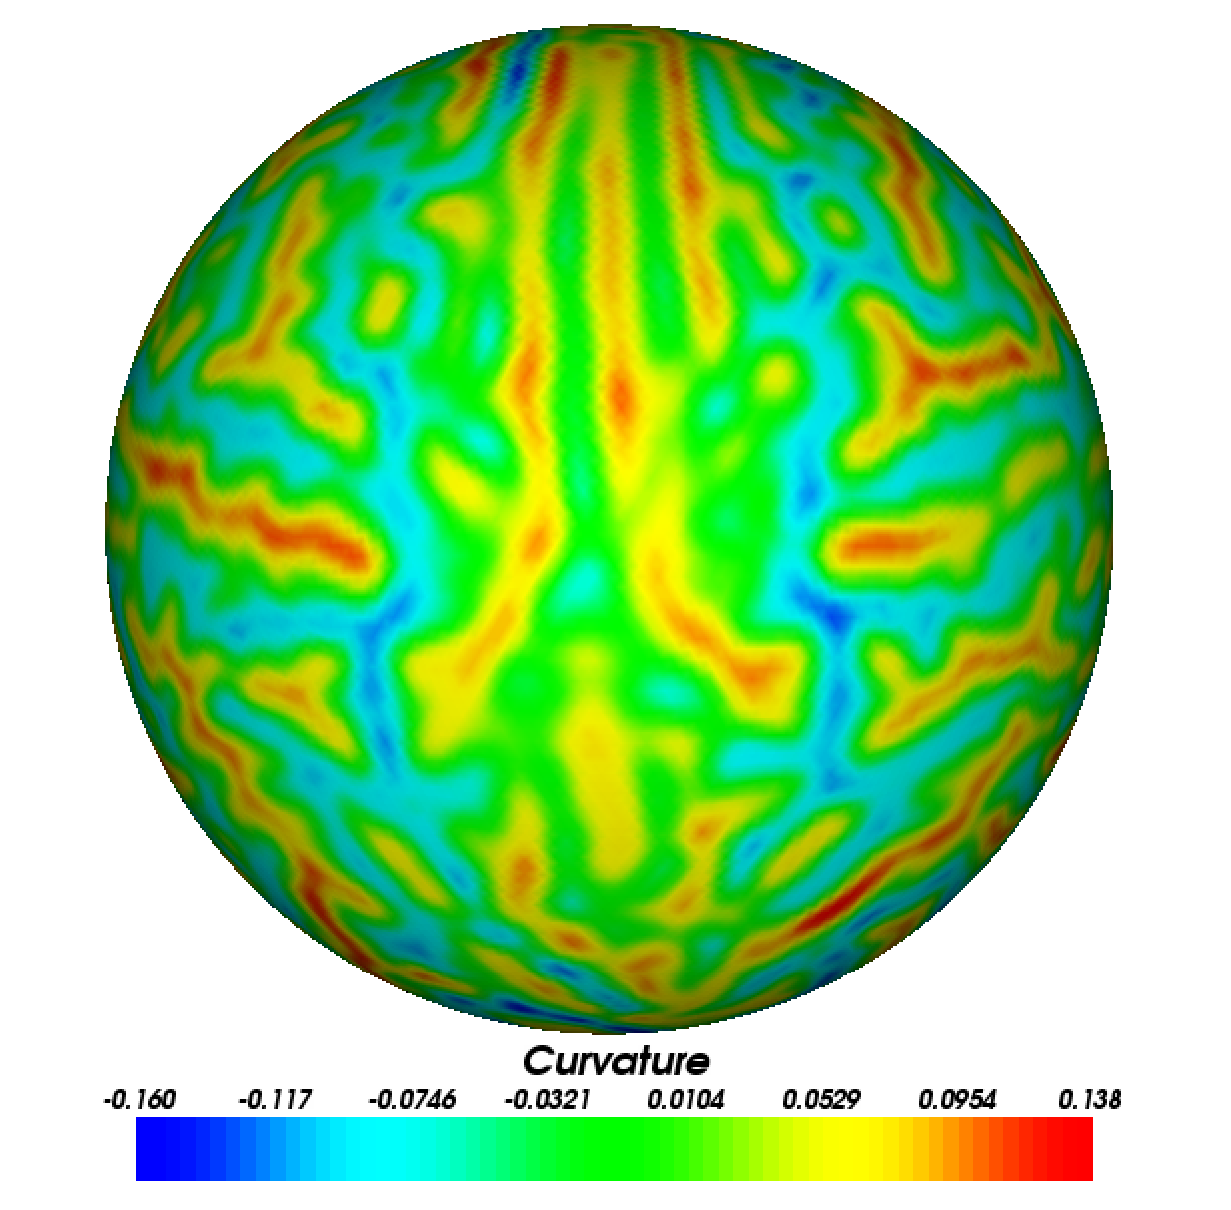
\includegraphics[%
  width=0.5\linewidth,
  keepaspectratio]{00111_smooth_32.ps}\tabularnewline
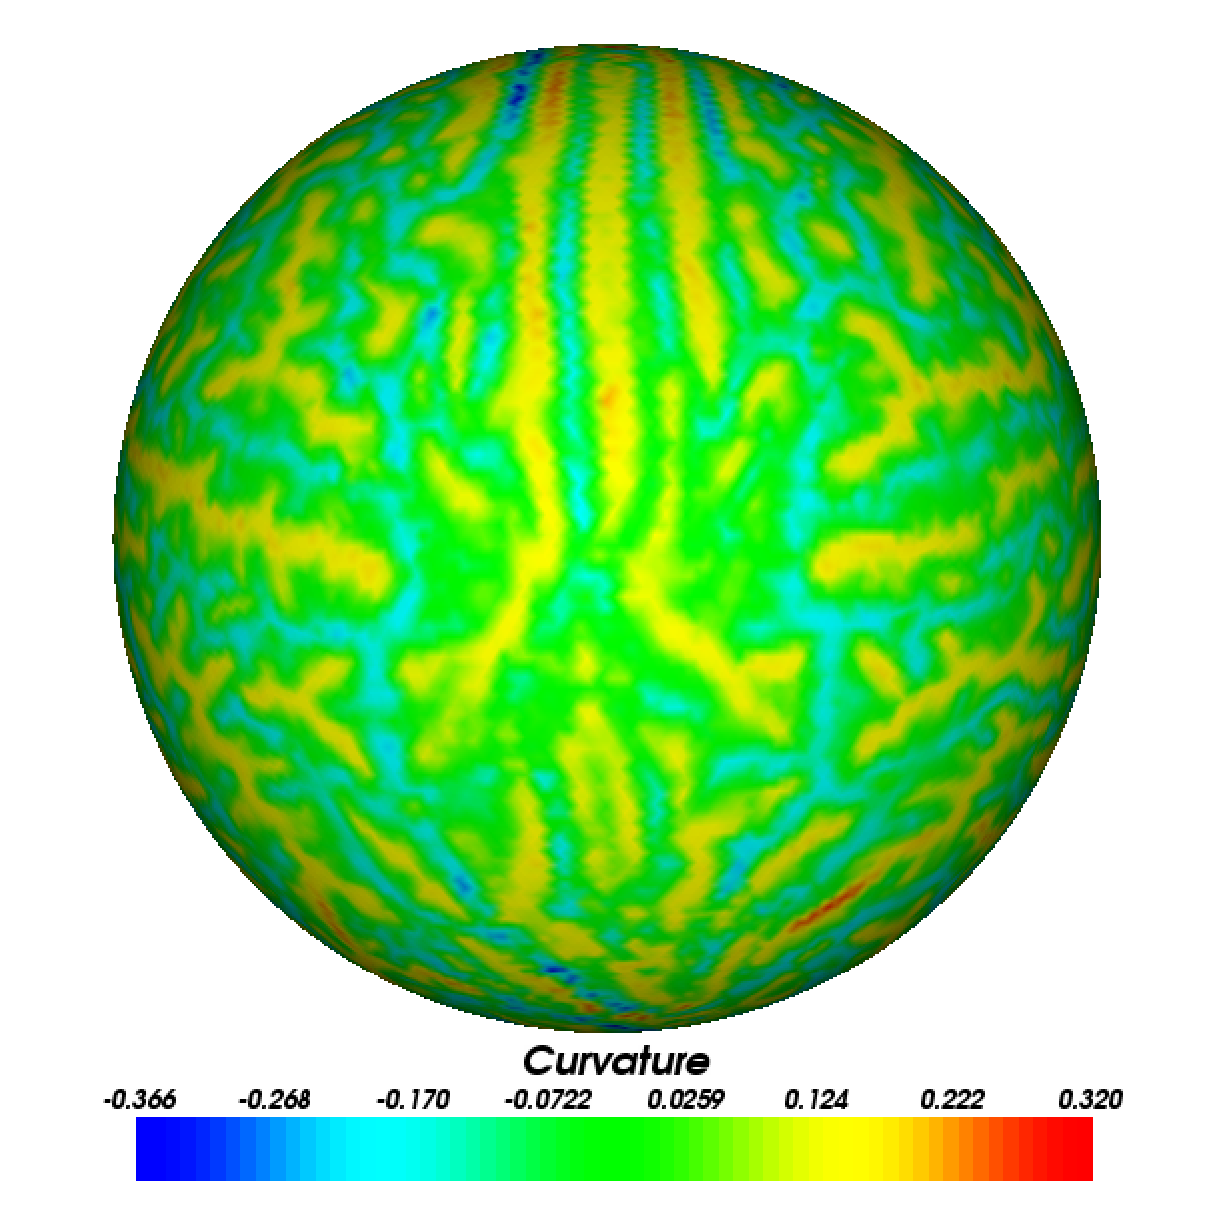
\includegraphics[%
  width=0.5\linewidth,
  keepaspectratio]{00111_smooth_8.ps}&
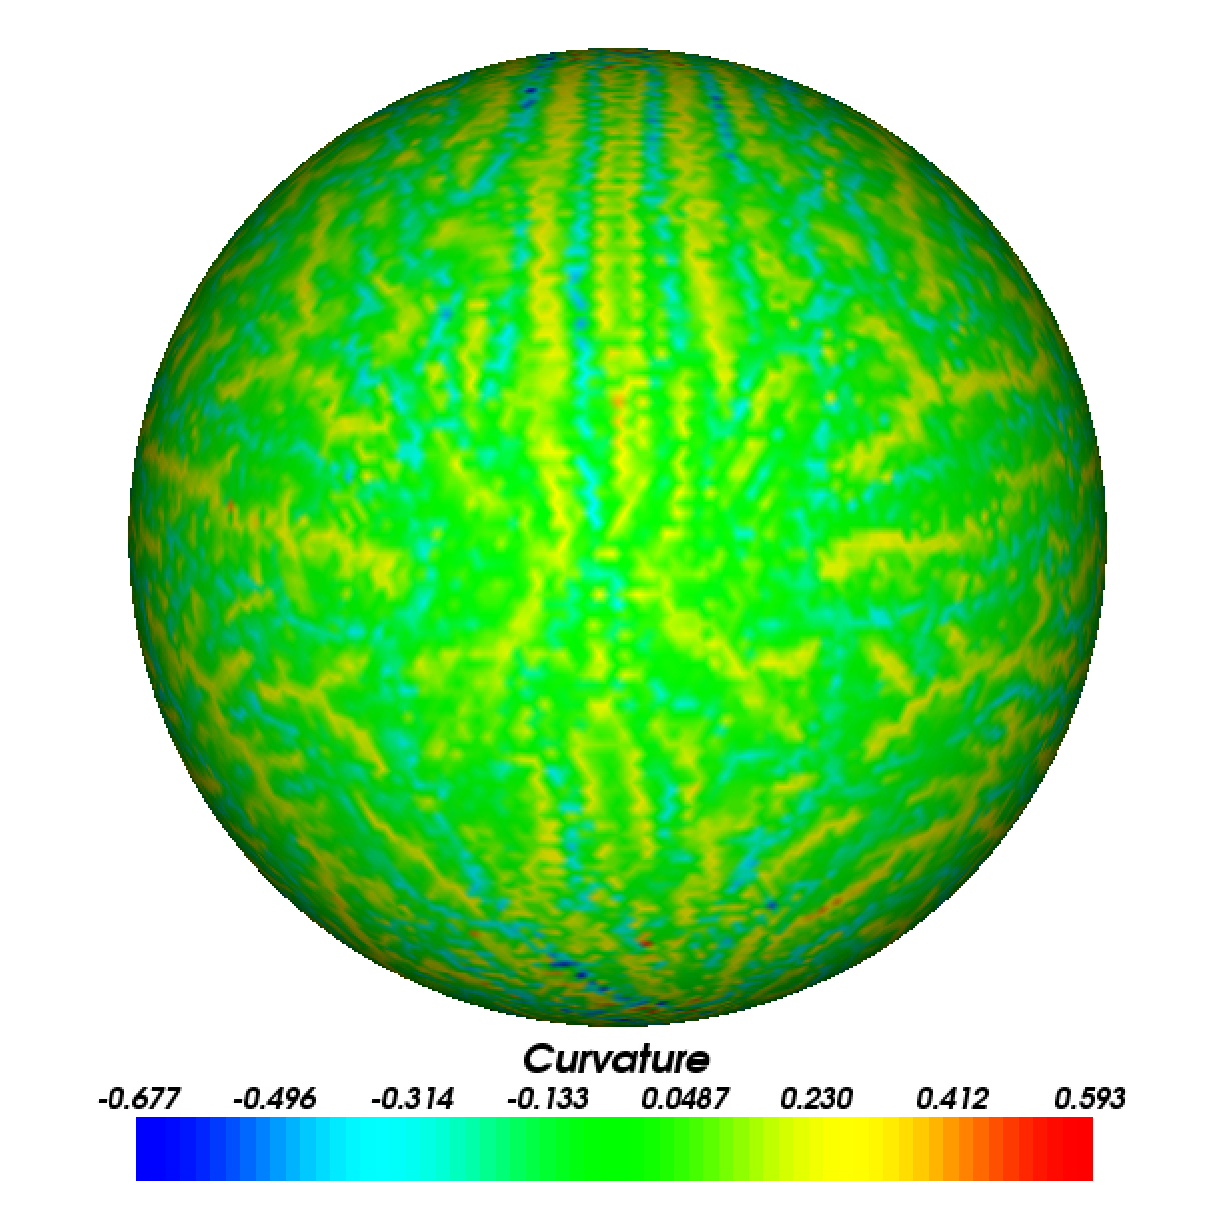
\includegraphics[%
  width=0.5\linewidth,
  keepaspectratio]{00111_smooth_2.ps}\tabularnewline
\end{tabular}\end{center}


\subsection{Inner Loop}

The optimization perfomed at each step of the coarse-to-fine outer
loop is the two-step Algorithm \ref{alg:Two-Step-Registration}, which
we call the inner loop.


\subsubsection{Matching (Step 2)}

The data term is written as a sum of terms, one for each vertex, $\Phi_{D}(U)=\sum_{v}\phi^{v}(U)$.
Each term is based on the correlation coefficient similarity measure
\cite{roche00:max-likelihood}, that produces a value in range $[-1,1]$
with better match indicated by larger score. Since \noun{surftracc}
operates as a minimization, we need to invert this\[
\phi^{v}(U)=1-\phi_{CC}^{v}(U),\]
where $\phi_{CC}^{v}$ is the correlation coefficient evaluated between
a neighbourhood of $v$ on the source data and a neighbourhood of
$U(v)$ on the target data. 

Each neighbourhood is a spherical cap at the given centre point $p$,
where $p$ is either $v$ or $U(v)$. The correlation coefficient
is evaluated by sampling on a set of sample points in each neighbourhood.
The sample points are arranged on a disc of radius $R_{n}$ parallel
to the tangent plane at $p$, as illustrated below. 

\begin{center}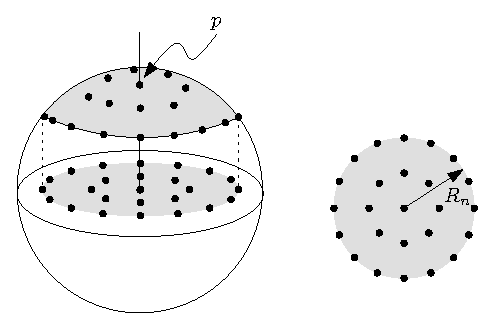
\includegraphics[%
  width=1\linewidth]{similarity-neighbourhood.eps}\end{center}

The set of sample points are: the centre of the disc, 8 points equally
spaced around a circle of radius $R_{n}/2$, and 16 points equally
spaced on a circle of radius $R_{n}$. The disc radius is \begin{equation}
R_{n}=r_{n}d_{C},\label{eq:define-neighbourhood-radius}\end{equation}
 where $r_{n}$ is a user-specified radius factor, and $d_{C}$ sets
the distance scale based on the coarseness of the control mesh. The
value of $d_{C}$ is the distance, projected to the disc, from the
centre of the cap to a neighbouring control mesh vertex. In other
words, $d_{C}$ is the length of a typical control mesh edge after
projecting to the disc. The value of $R_{n}$ must be no greater than
1, so $r_{n}\le1/d_{C}$.

The penalty $\Psi$ is also written as a sum over nodes of the control
mesh, $\Psi(T-U)=a\sum_{v}\psi(||T(v)-U(v)||)$. The penalty function
$\psi$ is designed so that $U(v)$ is restricted to the hemisphere
centred on $T(v)$. This is easily done by choosing $\psi$ such that
it becomes infinite when the angle between $T(v)$ and $U(v)$ reaches
$\pi/2$. 

With the search space restricted to a hemisphere, it can be parameterized
using two variables, by projecting the points on the sphere to the
tangent plane at $T(v)$. Thus, $U(v)$ is obtained using a two-dimensional
unconstrained optimization. Points $T(v)$ and $U(v)$ are projected
to this disc and $r$ is defined as the distance between the projected
points as illustrated.

\begin{center}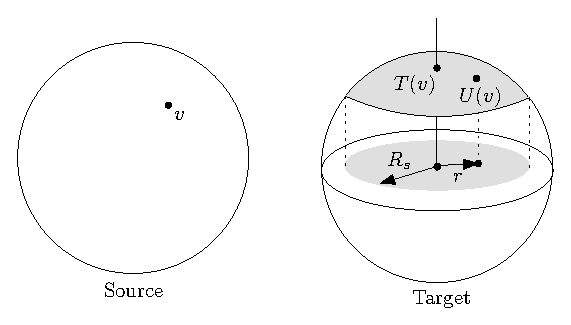
\includegraphics[%
  width=1\linewidth]{search-neighbourhood.eps}\end{center}

The penalty is a logarithmic barrier function \cite{nocedal99:numerical-optimization},
$\psi=-\log(1-r^{2}/R_{s}^{2})$, which has the effect of constraining
the search for $U(v)$ to points with $r<R_{s}$. The disc radius
is \begin{equation}
R_{s}=r_{s}d_{T},\label{eq:define-search-radius}\end{equation}
 where $r_{s}$ is a user-specified search radius factor, and $d_{T}$
sets the distance scale based on the control mesh. The value of $d_{T}$
is the distance, projected to the disc, between $T(v)$ and $T(u)$
where $u$ is the control-mesh neighbour closest to $v$ on the target,
i.e. $||T(v)-T(u)||$ is minimum for all 1-ring neighbours $u$ of
$v$. The value of $R_{s}$ must be no greater than 1, so $r_{s}\le1/d_{T}$.

The objective function is designed to be separable so that the minimization
of \begin{equation}
\phi^{v}(U(v))+a\psi(||U(v)-T(v)||)\label{eq:objective-vertex-v-2d}\end{equation}
 is performed independently for each control mesh vertex $v$. Each
optimization is a 2-dimensional problem, parameterized by Cartesian
coordinates in the tangent plane at $T(v)$. The initial iterate is
$(0,0)$ which corresponds to $T(v)$, and is a feasible point since
it corresponds to $r=0$ so the barrier function $\psi$ is zero.
The optimization is performed using the Nelder-Mead downhill simplex
algorithm \cite{press88:numerical-recipes} as implemented in the
GNU Scientific Library \cite{galassi02:gsl-book}. The Nelder-Mead
simplex algorithm is chosen because it does not require derivatives
of the objective function \ref{eq:objective-vertex-v-2d}, which are
complicated due to the correlation coefficient data term in $\phi^{v}$. 


\subsubsection{Smoothing (Step 3)}

The smoothing, which is carried out in $\Rthree$, is a simple weighted
average of $U(v)$ and the centroid of its neighbourhood, \[
C(v)=\frac{1}{|N_{v}|}\sum_{u\in N_{v}}U(u),\]
where $N_{v}$ is the set of neighbours of $v$. The smoothed transformation
is given by \[
T(v)=\frac{U(v)+wC(v)}{||U(v)+wC(v)||},\]
where $w$ is a user-specified smoothing weight.


\subsection{Algorithm Parameters}

The user of this algorithm has four major parameters to specify: the
search radius $r_{s}$, the neighbourhood radius $r_{n}$, the penalty
ratio $a$, and the smoothing weight $w$. Note that the search radius
and neighbourhood radius are dimensionless quantities that multiply
a length set by the coarseness of the control mesh through Equations
\ref{eq:define-neighbourhood-radius} and \ref{eq:define-search-radius},
respectively. Thus $r_{s}$ and $r_{n}$ can be set to a fixed value
for all iterations of the outer coarse-to-fine loop, as are parameters
$a$ and $w$.


\section{Output}

The output is a map $T:\Stwo\rightarrow\Stwo$, specified in a piecewise
linear fashion by providing $T(v)$ for all vertices $v$ of the control
mesh. The transformation at vertex $v$ is a point $T(v)\in\Stwo$.
However, instead of storing the Euclidean coordinates for the point
$T(v)$, the triple $(h,\alpha,\beta)$ is stored where $h$ is a
halfedge (internally represented as a pointer) specifying the spherical
triangle of the target data mesh that contains $T(v)$ and $(\alpha,\beta)$
are the areal coordinates (along with $\gamma\equiv1-\alpha-\beta$)
locating $T(v)$ on the spherical triangle as illustrated.

\begin{center}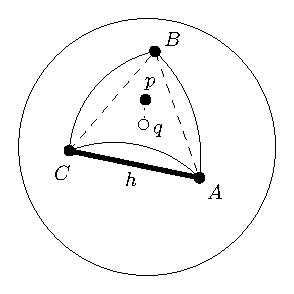
\includegraphics{surfacepoint.eps}\end{center}

%% LyX 1.3 created this file.  For more info, see http://www.lyx.org/.
%% Do not edit unless you really know what you are doing.
\documentclass[10pt,letterpaper,twocolumn,english]{article}
\usepackage{ae}
\usepackage{aecompl}
\usepackage[T1]{fontenc}
\usepackage[latin1]{inputenc}
\usepackage{float}
\usepackage{amsmath}
\usepackage{graphicx}
\usepackage{amssymb}

\makeatletter

%%%%%%%%%%%%%%%%%%%%%%%%%%%%%% LyX specific LaTeX commands.
\newcommand{\noun}[1]{\textsc{#1}}
%% Because html converters don't know tabularnewline
\providecommand{\tabularnewline}{\\}
\floatstyle{ruled}
\newfloat{algorithm}{tbp}{loa}
\floatname{algorithm}{Algorithm}

%%%%%%%%%%%%%%%%%%%%%%%%%%%%%% User specified LaTeX commands.
\usepackage{url}

\newcommand{\inlinedef}[1]{\emph{#1}\index{#1}\glossary{#1}}
\newcommand{\sphericaltri}{\textcircled{$\triangle$}}

\usepackage{babel}
\makeatother
\begin{document}

\title{The Theory and Practice of Non-Rigid Surface Warping}


\author{Steven M. Robbins}

\maketitle

\newcommand{\Real}{\mathbb{R}}

\newcommand{\Rthree}{\mathbb{R}^{3}}

\newcommand{\Stwo}{\mathbb{S}^{2}}



\section{Introduction}

Surface registration is a procedure that produces a spatial mapping
from one surface, which we call the \emph{source} surface, to a second,
\emph{target}, surface. This manual is not a treatise on surface registration
(see, e.g. \cite{robbins03:phd}) but only documents the specific
theory and practice underlying \noun{surftracc}. 


\section{Input Data}

The input to surface registration is a pair of surfaces such as those
generated from a 3D MR image using software such as \noun{asp}/\noun{clasp}\cite{macdonald00:cortical-surfaces}.
In adition, a feature data function for each surface is required.


\subsection{Surface Description}

Each input surface must be a triangulated polyhedral surface, also
called a \emph{mesh}. Further, \noun{surftracc} assumes that the
surface has a very specific structure as follows.

First of all, \noun{surftracc} requires that the mesh represent
a topological sphere, i.e. a closed surface that bounds a finite volume
of space.

A common way to refine a mesh is by quadrisection, in which each triangle
is replaced by four triangles by joining the midpoints of the three
edges, as shown.

\begin{center}\includegraphics{quadrisection.eps}\end{center}

In addition to being a topological sphere, \noun{surftracc} requires
that the mesh graph be a repeated quadrisection of an icosahedron,
the graph with 20 triangular faces and 12 vertices each of degree
five. Each quadrisection increases the number of faces by a factor
of four. The following table shows the number of faces and vertices
produced by repeated quadrisection.

\begin{center}\begin{tabular}{|c|c|c|}
\hline 
\# Quadrisections&
\# Faces&
\# Vertices\tabularnewline
\hline
\hline 
0&
20&
12\tabularnewline
\hline 
1&
80&
42\tabularnewline
\hline 
2&
320&
162\tabularnewline
\hline 
3&
1280&
642\tabularnewline
\hline 
4&
5120&
2562\tabularnewline
\hline 
5&
20480&
10242\tabularnewline
\hline 
6&
81920&
40962\tabularnewline
\hline 
7&
327680&
163842\tabularnewline
\hline
\end{tabular}\end{center}

Note that ASP/CLASP outputs surfaces of the form required by \noun{surftracc}.


\subsection{Match Feature}

Along with each surface, we need data to determine how the surfaces
match. The basic idea is to define a scalar \emph{feature} function
on each surface such that a matching region on the source and target
have a similar feature pattern. The feature values needn't match exactly
since, as described below, we use a correlation similarity measure
to drive the optimization.

The feature function is defined in a piecewise-linear fashion by providing
the function value at each vertex. At other points on the surface,
the function is interpolated from the 3 values at the triangle vertices.
This interpolation is described in more detail later.

We next describe two geometric feature functions that can be used
for registration: mean curvature and crown distance transform.


\subsubsection{Curvature}

The mean surface curvature is a popular choice for match feature since
gyral crowns and sulcal fundii have curvature of different sign. So
matching curvature should match gyrus to gyrus and sulcus to sulcus.

This Figure shows the value of mean curvature evaluated (using \cite{taubin95:estimating-curvature})
at each vertex of the cortical surface.

\begin{center}\begin{tabular}{cc}
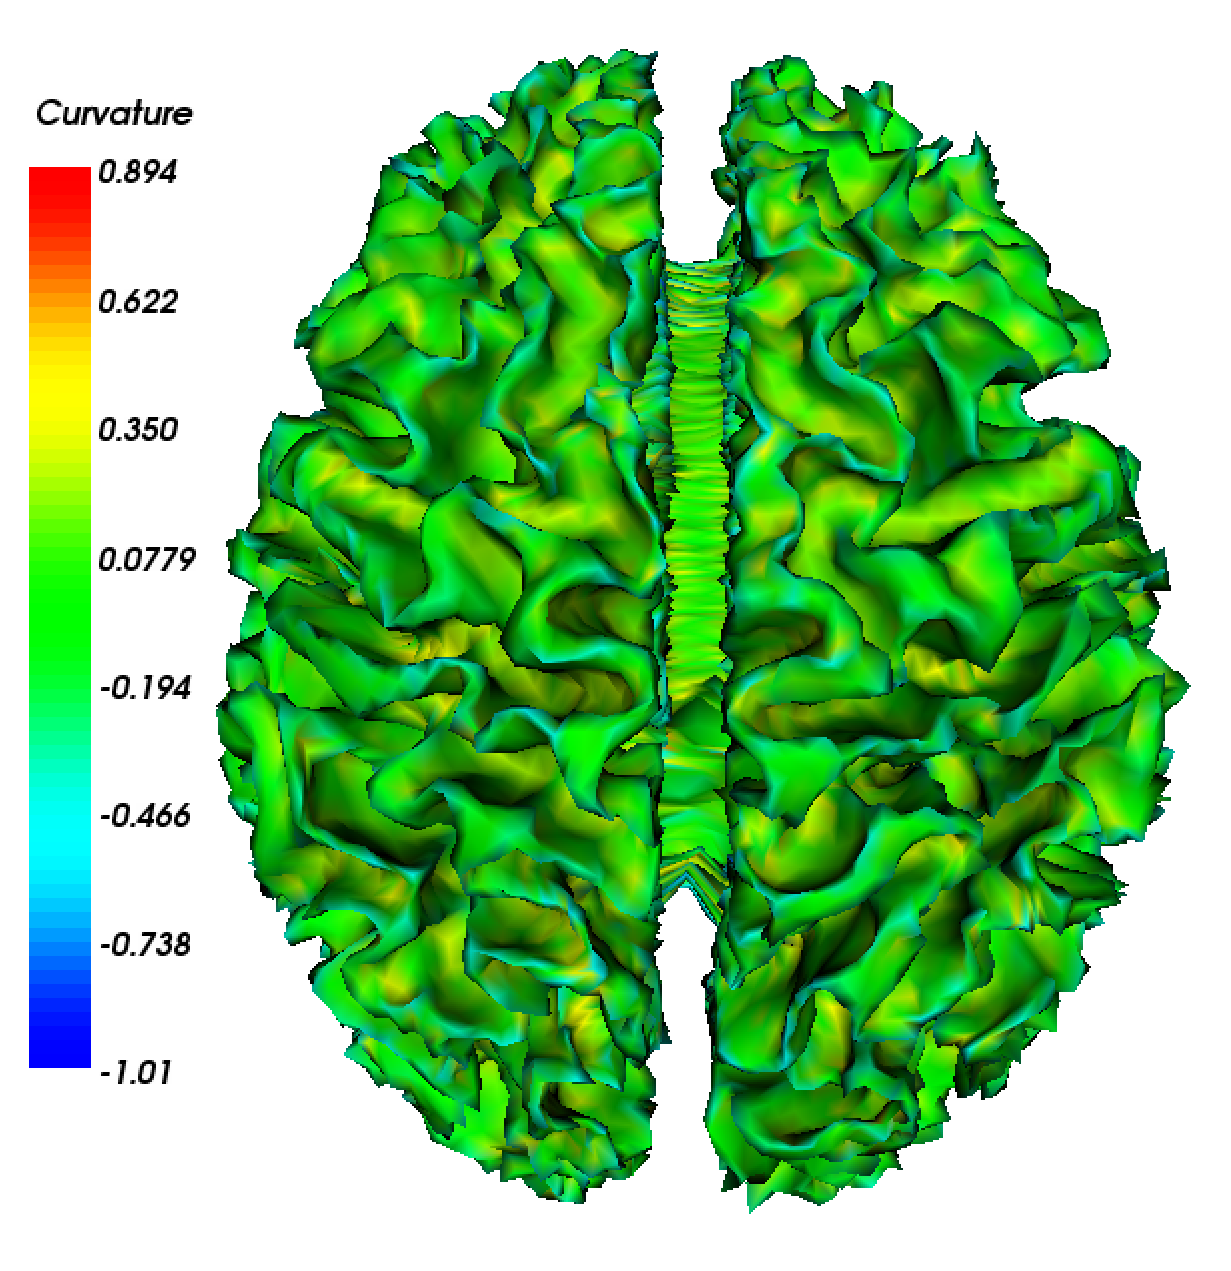
\includegraphics[%
  width=0.45\linewidth,
  keepaspectratio]{mean-cortex-top.ps}&
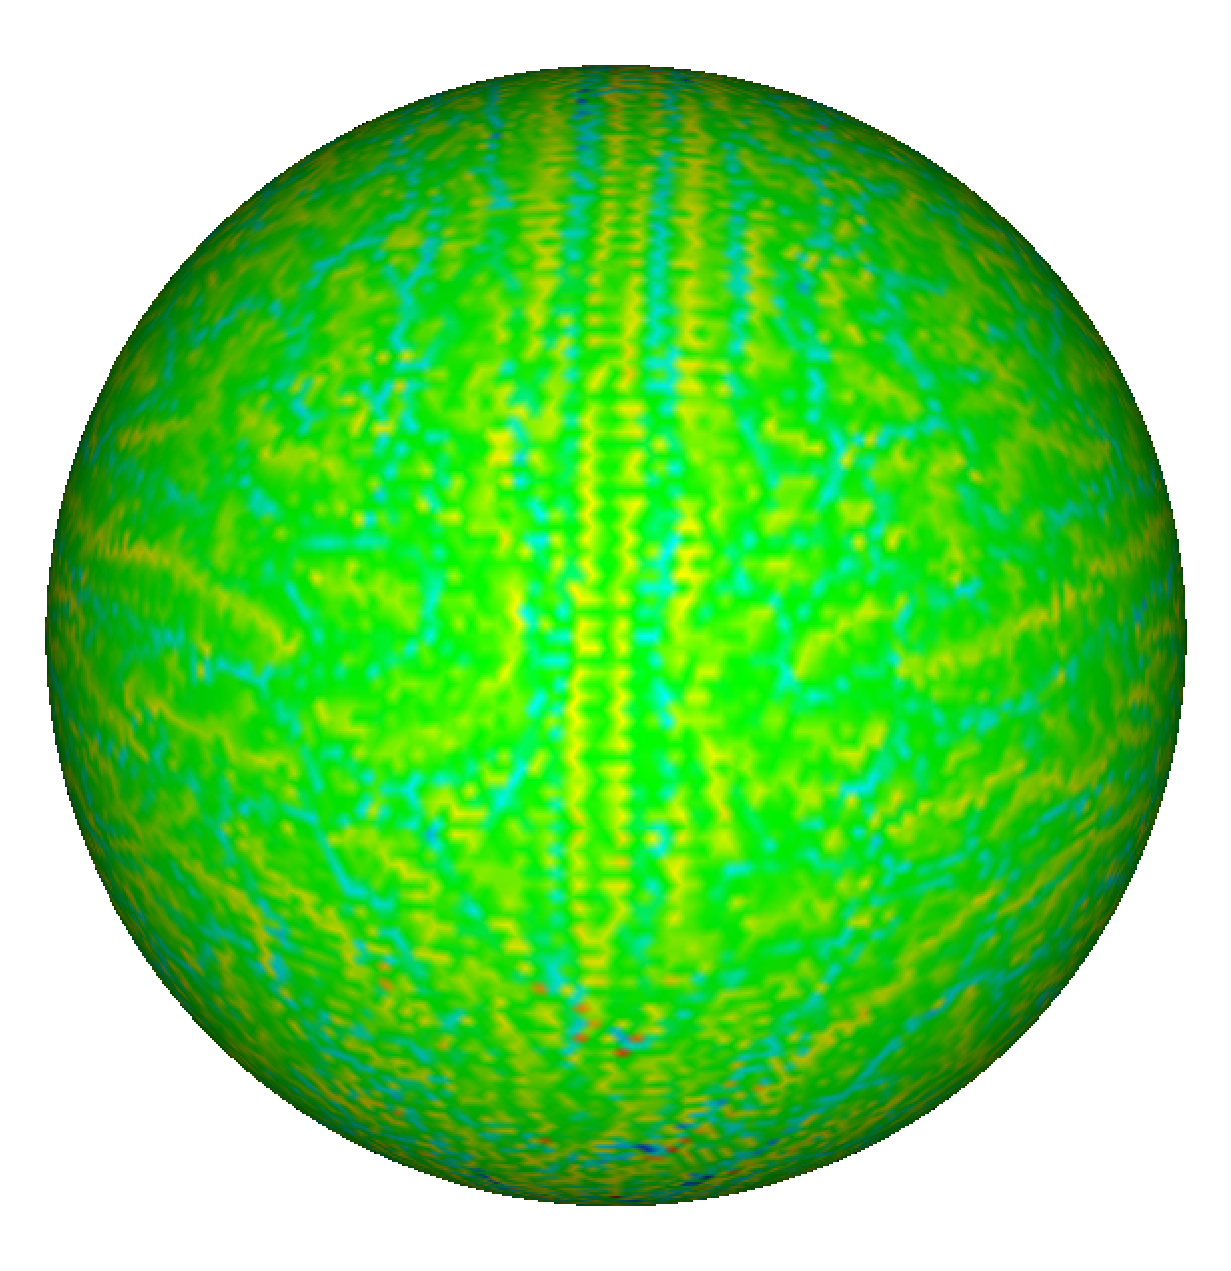
\includegraphics[%
  width=0.45\linewidth,
  keepaspectratio]{mean-sphere-top.ps}\tabularnewline
\end{tabular} \end{center}

Since sulcal fundi and gyral crowns have mean curvature of opposite
sign, registration based on matching mean curvature should tend to
match sulcus to sulcus and gyrus to gyrus. However, there is evidently
a lot of noise in the curvature map as well, due to small-scale oscillations
in the mesh vertex positions, so the data needs to be smoothed when
used for registration, either by smoothing the surface before computing
the curvature, or by directly averaging function values in a neighbourhood
of each vertex.


\subsubsection{Crown Distance Transform}

The intuition behind this feature, like that of mean curvature, is
that it is desirable to match points along the crown of a gyrus on
the source surface with points along the crown of a gyrus in the target
surface. Similarly, the fundus of a sulcus should match the fundus
of a sulcus. In contrast to matching by mean curvature, other points
on the bank of a sulcus are matched according to their fractional
distance towards the bottom of the sulcus, e.g. a vertex halfway down
the sulcus in the source mesh should match a point halfway down the
target sulcus.

Suppose vertex $v$ is located in a sulcus of the source mesh. Consider
two shortest geodesic paths, one from $v$ to the gyral crown and
the other from $v$ to the fundus. Let the length of the first of
these paths be $S(v)$ and let $S_{D}(v)$ be the sum of the two path
lengths. Distance $S_{D}(v)$ can be regarded as the depth of the
sulcus along a path through $v$. Let $R$ and $R_{D}$ be the analogous
distance functions for the target surface. The fractional depth of
vertex $v$ on the source mesh is $S(v)/S_{D}(v)$.

\begin{center}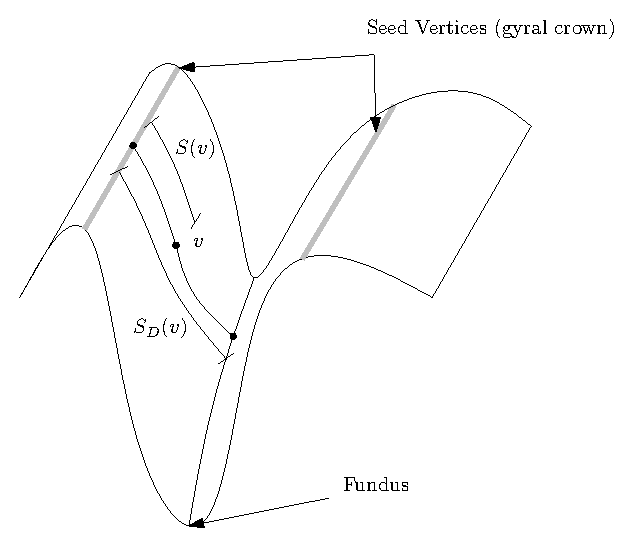
\includegraphics[%
  width=0.9\columnwidth,
  height=0.2\paperwidth,
  keepaspectratio]{fractional-depth.eps}\end{center}

The desired matching is to a point $T(v)$ on the target surface such
that $S(v)/S_{D}(v)\approx R(T(v))/R_{D}(T(v))$, or\begin{equation}
R(T(x))=\alpha(x)+\beta(x)S(x)+\epsilon(x),\label{eq:dt-matching-relation}\end{equation}
 where $\epsilon$ represents random noise, $\beta(x)=R_{D}(T(x))/S_{D}(x)$,
and $\alpha$ should be zero. However, $\alpha$ is left free to compensate
for practical difficulties in computing $S(x)$ and $R(x)$. Note
that points near to $v$ should have depth values close to $S_{D}(v)$
and similarly points near $T(v)$ should have depth values close to
$R_{D}(T(v))$. Assuming that $\alpha$ and $\beta$ are slowly-varying
functions, the maximum likelihood estimate for $T$ corresponds to
maximizing the regional correlation coefficient \cite{robbins03:phd}. 

Note that only the gyral crown distance functions, $S$ and $R$ appear
in Equation~\ref{eq:dt-matching-relation} and not $S_{D}$ and $R_{D}$.
Thus, the feature value stored at each vertex is the geodesic \emph{distance
transform} from a set of gyral {}``seed'' vertices, i.e. the length
of the shortest geodesic path from $v$ to a vertex in the seed set.


\paragraph{Seed Points}

The vertices chosen to be the seeds should in principle be all vertices
located on all the gyral crowns. We can identify gyral vertices with
the help of an \emph{$\alpha$-shape} \cite{edelsbrunner94:alpha-shapes},
a discrete geometry notion that can be considered as a relaxation
of the convex hull. The degree of relaxation is controlled by the
parameter $\alpha$ in the following manner. Let $S$ be a set of
points in $\Rthree$. Define an \emph{$\alpha$-ball}%
\footnote{The definition given here follows the Computational Geometry Algorithms
Library (CGAL) \cite{cgal-web}, as the implementation of $\alpha$-shape
provided by CGAL is used. In the original definition of Edelsbrunner
and M�cke, $\alpha$ is the radius of the $\alpha$-ball.%
} to be a closed ball of radius $\sqrt{\alpha}$, i.e. the point set
$\{ x\in\Rthree:||x-p||\le\sqrt{\alpha}\}$, for some $p\in\Rthree$.
The points of $S$ that form the vertices of the $\alpha$-shape of
$S$ are those that lie on the boundary of an $\alpha$-ball with
no point of $S$ on the interior of the $\alpha$-ball. Such vertices
are said to be \emph{$\alpha$-exposed.} Note that convex hull vertices
are always $\alpha$-exposed, since for every point $x$ on the boundary
of a convex set, there exists a ball of radius $\sqrt{\alpha}$ for
any value of $\alpha$ that intersects the convex set only at $x$.
Thus the vertices of the $\alpha$-shape with $\alpha=\infty$ are
the vertices of the convex hull. As $\alpha$ is decreased, more points
become $\alpha$-exposed until at $\alpha=0$ all points are $\alpha$-exposed. 

Using $\alpha$-balls of radius 10 mm (i.e. $\alpha=100$), a value
empirically chosen using visual inspection of the results, produces
good outlines of several major gyri. However, there are also vertices
in the point set lying underneath the brain on the arbitrary {}``cap''
through the brain stem which should not form part of the seed set;
these vertices are masked out as follows. The distance transform is
computed using the convex hull points as the seed vertices and any
vertex with a distance transform value greater than 35 (a value chosen
empirically) is removed from the set of vertices of the $\alpha$-shape.
The remaining vertices form the seed set used for the crown distance
transform feature.


\paragraph{Geodesic Distance}

The distance transform used in practice is an approximation to the
geodesic distance, as computing true geodesic distance is computationally
costly and difficult to code robustly \cite{lanthier01:approx-weighted-shortest-path}.
The approximation is computed using the mesh graph with the weight
for each edge set to the Euclidean length of the edge. An additional
vertex, $s$, is inserted and attached to each seed vertex with a
zero weight edge. Then Dijkstra's single-source shortest path algorithm
\cite{cormen90:intro-algorithms} is run with $s$ as the source vertex.
To improve the accuracy of the approximation the mesh is refined before
running Dijkstra's shortest path algorithm. First, $m$ equally-space
extra points are inserted on each edge, then a new edge is inserted
for each pair of extra points that either (i) are adjacent on an original
edge, or (ii) are on different edges both of which are incident to
a common (original) facet. The approximate shortest path computed
by this algorithm consists of line segments which are either an edge
of the original surface, or cross a facet of the original surface
as shown.

\begin{center}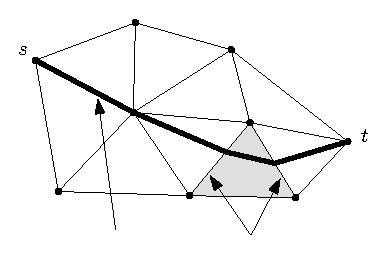
\includegraphics{approximate-path.eps}\end{center}

The crown distance transform from the final seed set is illustrated
below.

\begin{center}\begin{tabular}{cc}
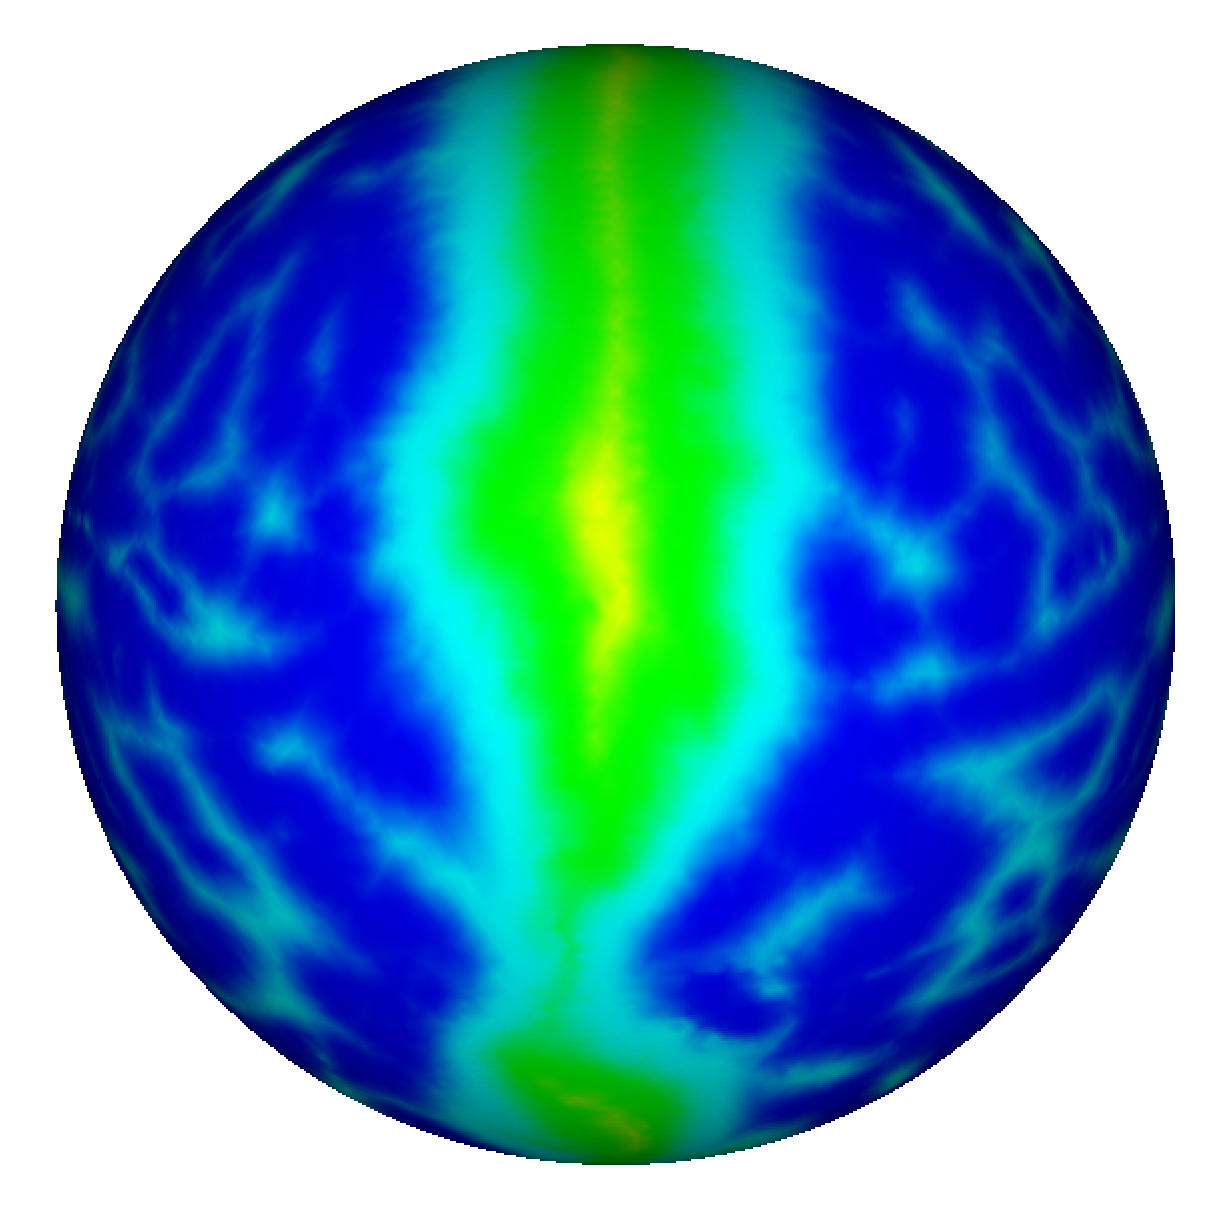
\includegraphics[%
  width=0.4\columnwidth,
  height=0.15\paperwidth,
  keepaspectratio]{sphere-top.ps}&
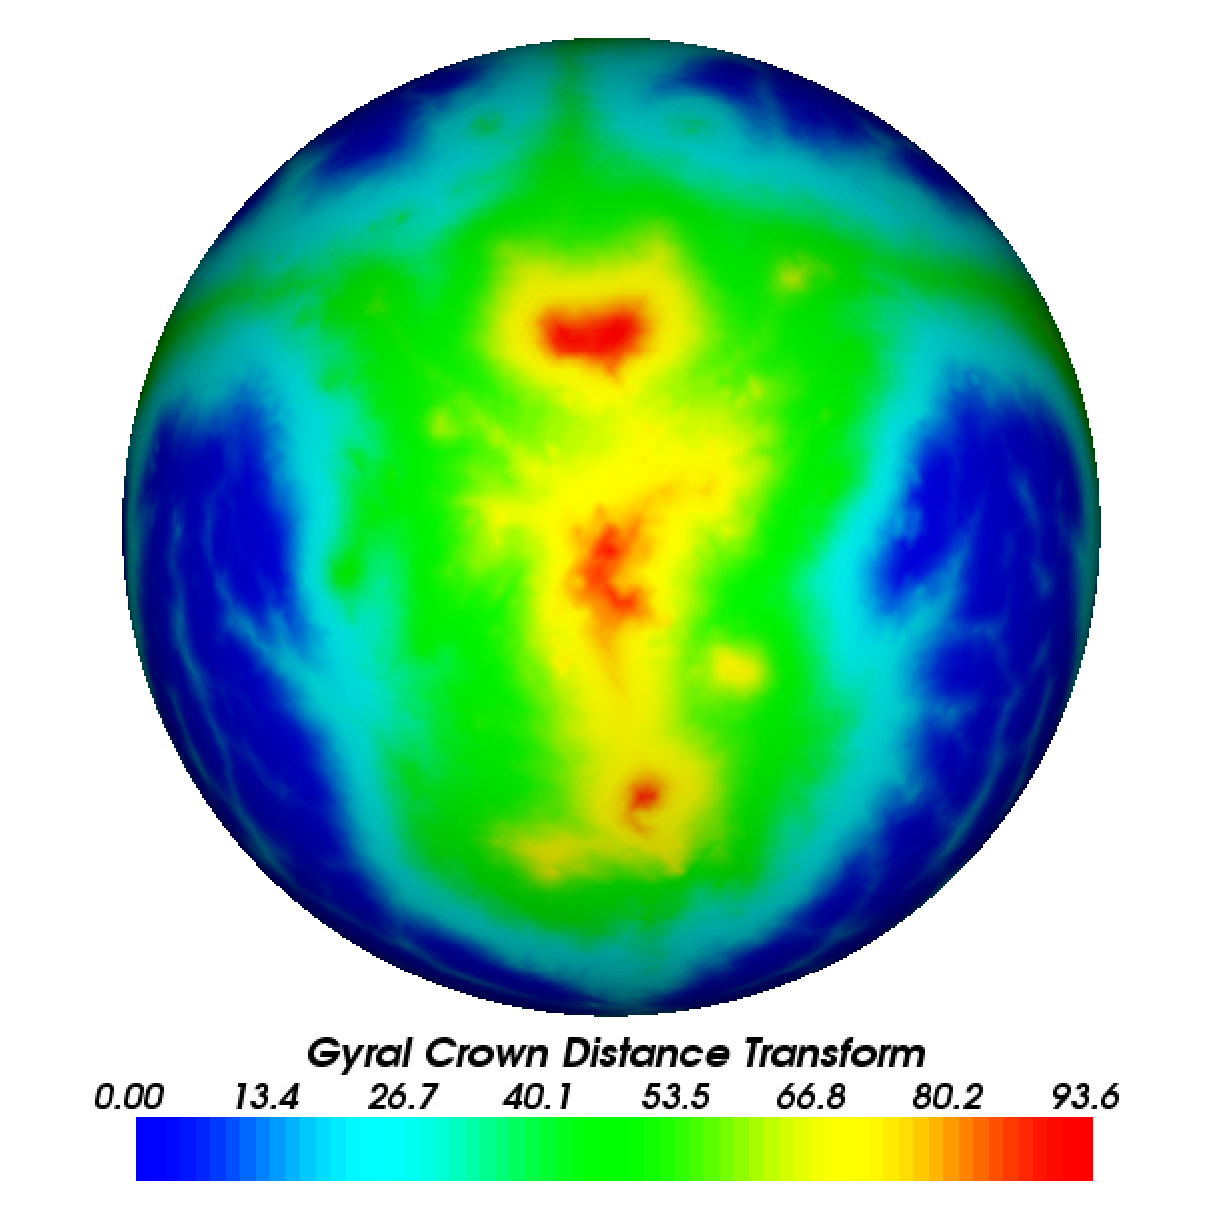
\includegraphics[%
  width=0.4\columnwidth,
  height=0.15\paperwidth,
  keepaspectratio]{sphere-bottom.ps}\tabularnewline
Top&
Bottom\tabularnewline
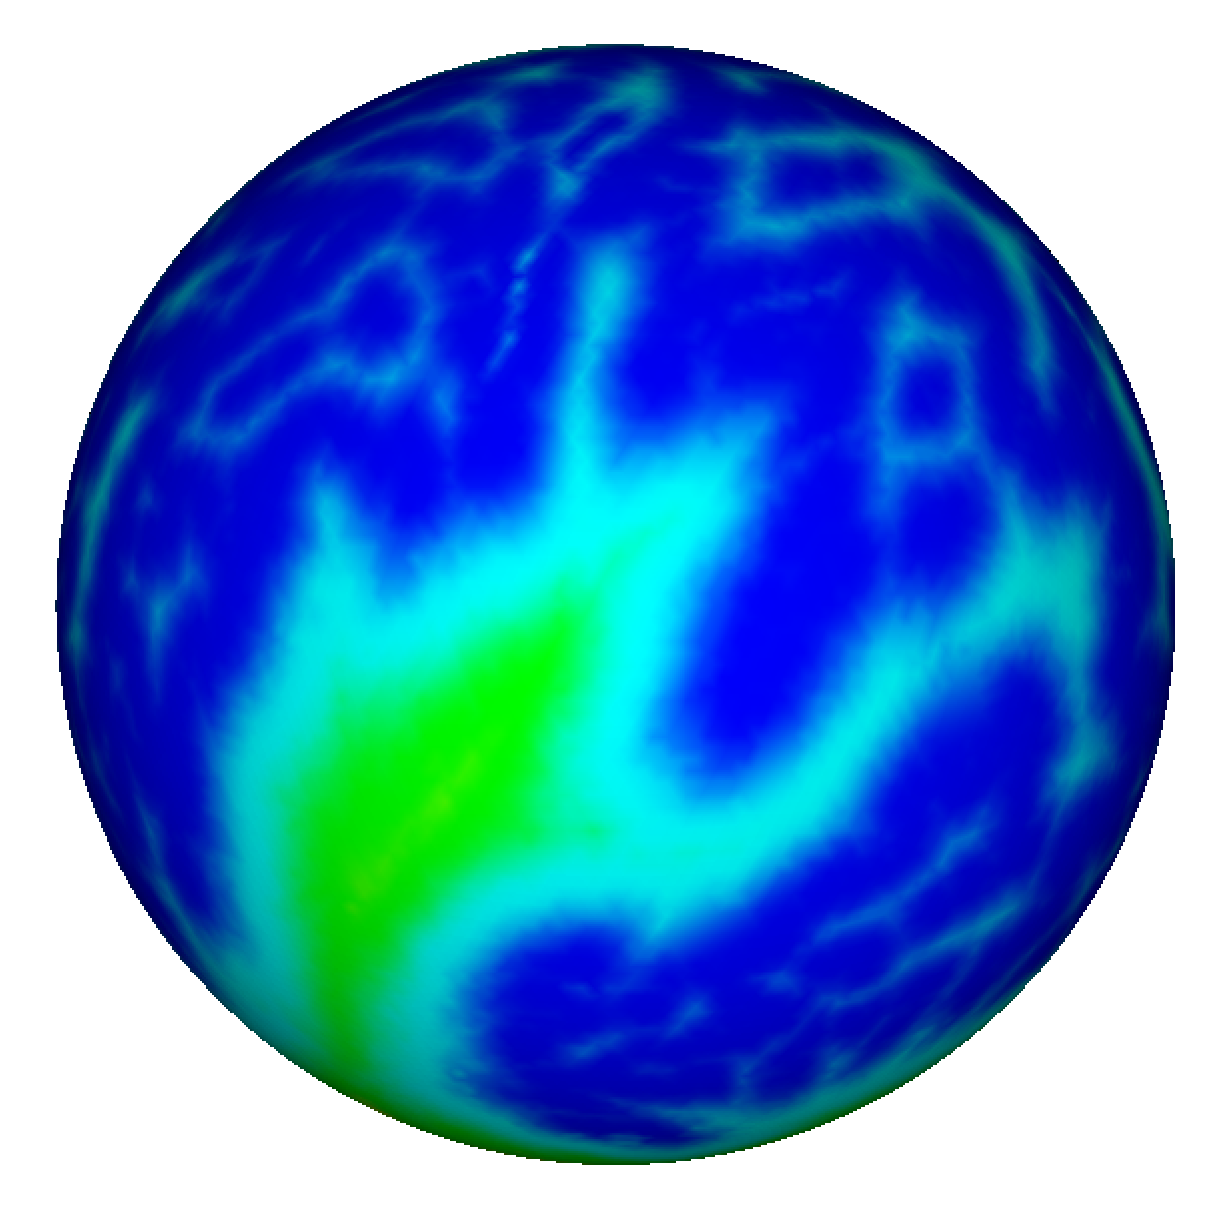
\includegraphics[%
  width=0.4\columnwidth,
  height=0.15\paperwidth,
  keepaspectratio]{sphere-left.ps}&
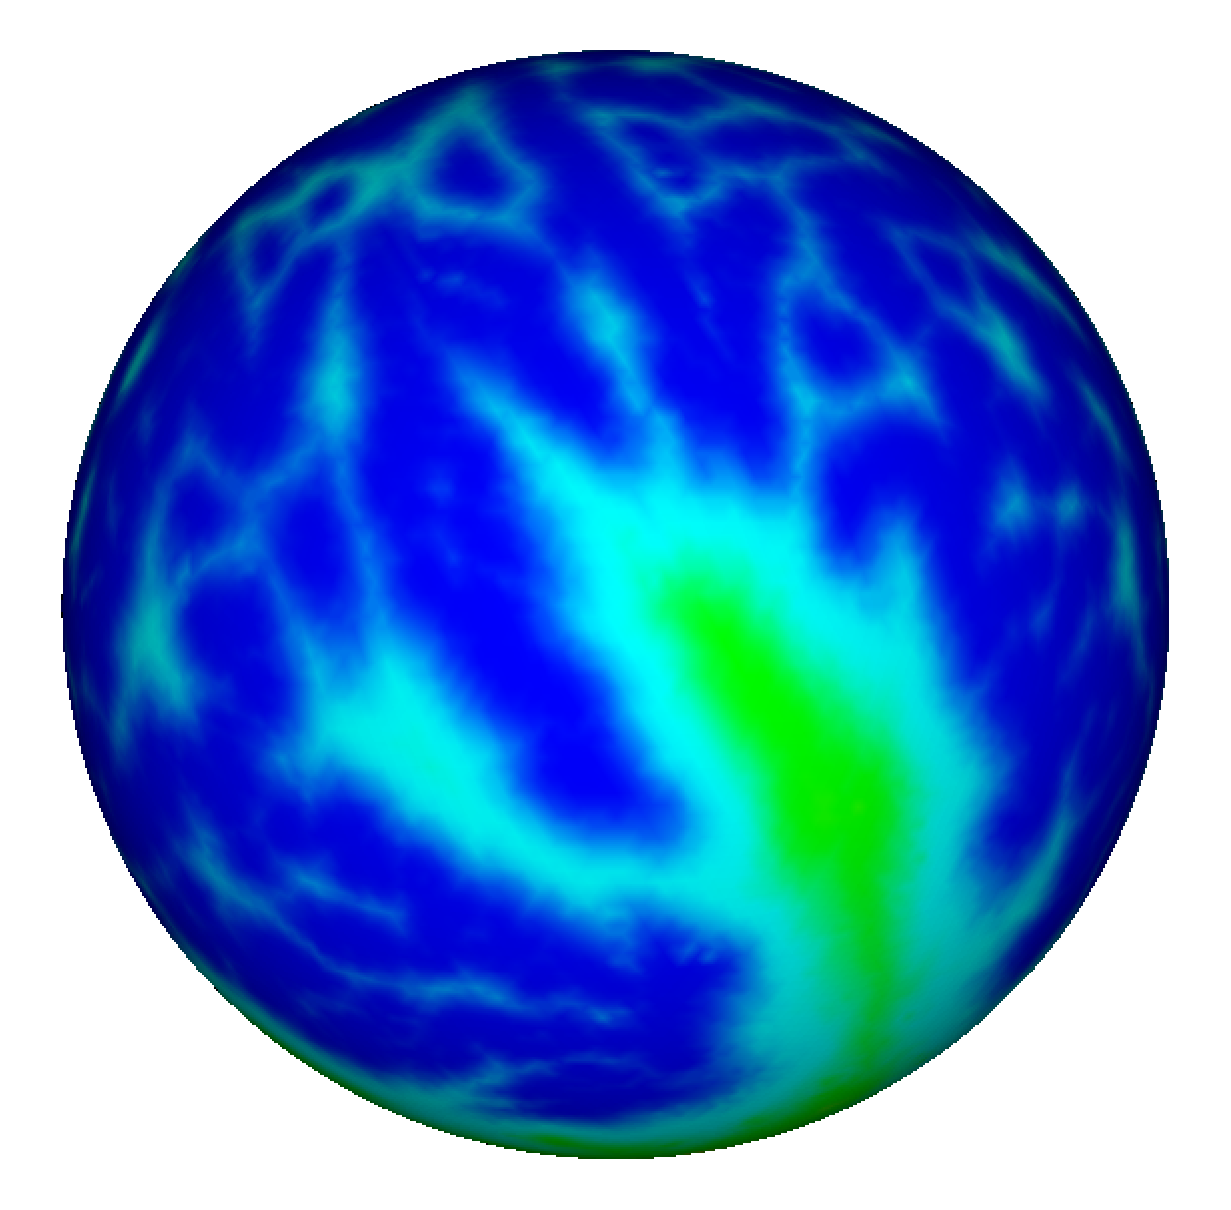
\includegraphics[%
  width=0.4\columnwidth,
  height=0.15\paperwidth,
  keepaspectratio]{sphere-right.ps}\tabularnewline
Left&
Right\tabularnewline
\end{tabular}\end{center}


\section{Triangle Interpolation}

Both the feature data function described above and, ultimately, the
transformation $T$ are defined at mesh vertices and interpolated
across the rest of the surface. We pause to discuss this interpolation
before discussing the optimization used to search for $T$.


\subsection{Scalar Function Interpolation}

Suppose that for a function, $f$, a real value is associated with
each vertex of the mesh, as is the case for the feature function data.
Let $p$ be a point on the mesh and consider what value to assign
$f(p)$. 

If $p$ is a vertex, the vertex value is assigned. 

If $p$ is not a vertex, let $ABC$ be a triangle of the mesh that
contains $p$. There is a unique triple of real values $(\alpha,\beta,\gamma)$
with $\alpha+\beta+\gamma=1$ that satisfies $p=\alpha A+\beta B+\gamma C$.
This triple is known as the \emph{areal coordinates} of $p$ \cite[section 13.7]{coxeter69:intro-geometry}.
We use these values for interpolation, assigning $f(p)=\alpha f(A)+\beta f(B)+\gamma f(C)$.
It is clear that this choice of interpolation (a) is consistent with
the assigned values at vertices $A$, $B$, and $C$, and (b) gives
consistent values along a shared triangle edge no matter which triangle
is used for the interpolation.


\subsection{Triangulation Warping}


\subsubsection{Auxiliary Space}

While it is conceivable to define the mapping $T$ directly on the
input mesh, it is easier to use a simpler auxiliary space instead;
\noun{surftracc} uses the unit sphere. The source mesh, $M_{I}$,
is first mapped to the sphere using an invertible projection map,
$\Pi_{I}$. This projection is given implicitly by the fact that $M_{I}$
is constrained to be a repeated quadrisection of the icosahedron,
as discussed above. The target surface $M_{J}$ is similarly projected
to the sphere by $\Pi_{J}$. The registration algorithm then computes
$T:\Stwo\rightarrow\Stwo$ which, together with the two projection
operations, serves to define map between the two input surface meshes,
denoted $W:M_{I}\rightarrow M_{J}$ in the diagram.

\begin{center}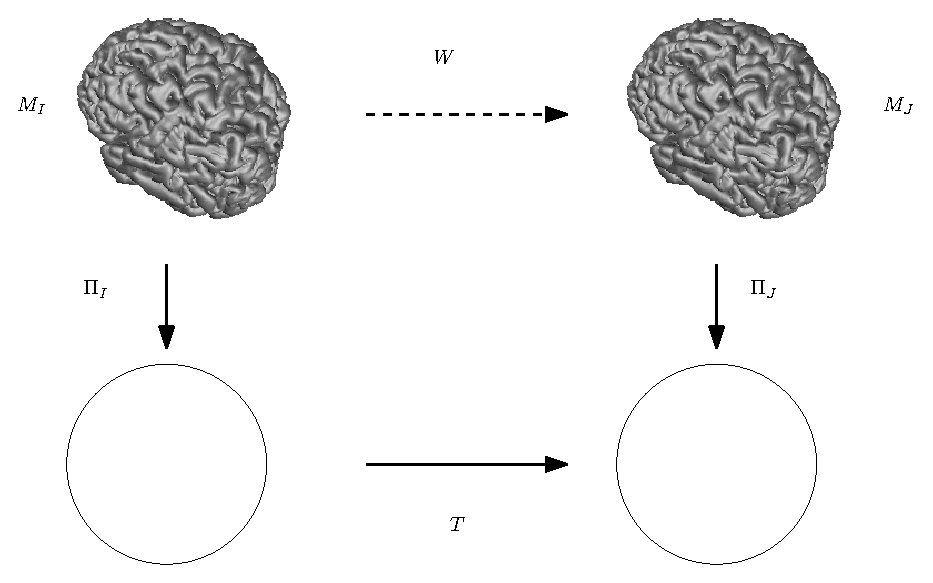
\includegraphics[%
  width=1\columnwidth,
  keepaspectratio]{mappings.eps}\end{center}


\subsubsection{Triangulation Warping on the Sphere}

We discuss now how the sphere-to-sphere mapping, $T:\Stwo\rightarrow\Stwo$
is defined. The basic idea is that the source sphere is partitioned
into spherical triangles, and the mapping under $T$ is given for
each spherical triangle. 


\paragraph{Mapping one Triangle}

Let $A$, $B$, and $C$ be three points on the sphere $\Stwo$ that
are not coplanar with the origin. Using projection from the origin,
i.e. the mapping $x\mapsto x/||x||$, the planar triangle $ABC$ is
put into 1-1 correspondence with a triangular patch of $\Stwo$ bounded
by three shortest geodesics, from $A$ to $B$, from $B$ to $C$,
and from $C$ to $A$. Each geodesic bounding the patch is denoted
an \emph{edge arc}, and the triangular patch of $\Stwo$ is known
as the \emph{spherical triangle} $\sphericaltri ABC$. Given the 1-1
mapping between the planar triangle $\triangle ABC$ and the spherical
triangle $\sphericaltri ABC$, areal coordinates can be used to refer
to either $q=\alpha A+\beta B+\gamma C\in\triangle ABC$ or to $p=q/||q||\in\sphericaltri ABC$.

The mapping of $\sphericaltri ABC$ begins by specifying the positions
of the vertices under the mapping; define $A'\equiv T(A)$, $B'\equiv T(B)$,
and $C'\equiv T(C)$. Define a mapping from point $p$ in spherical
triangle $\sphericaltri ABC$ to point $T(p)$ in spherical triangle
$\sphericaltri A'B'C'$ as follows. First, project $p$ to point $q$
on the planar triangle $ABC$ and compute the areal coordinates of
$q$. We define the corresponding point $q'\in\triangle A'B'C'$ using
$q'\equiv\alpha A'+\beta B'+\gamma C'$. Finally, $q'$ is projected
to point on the sphere, denoted $p'$ and we define $T(p)$ to be
$p'$. 

\begin{center}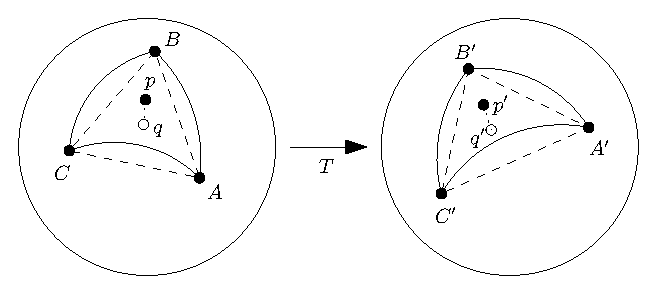
\includegraphics[%
  width=1\columnwidth,
  keepaspectratio]{trianglemap-sphere.eps}\end{center}


\paragraph{Mapping the Entire Sphere}

In order to map the entire sphere, all we need is a partitioning of
the sphere into a set of non-overlapping spherical triangles. For
each triangle, we use the procedure just described to map it. Since
each point of the input sphere is contained in at least one triangle,
a mapping of the sphere is achieved. As is the case when interpolating
real values, the interpolation of $T$ is consistent at vertices and
along edges of each spherical triangle. The overall mapping $T$ is
1-1 and invertible if it satisfies certain conditions \cite{robbins03:phd}.
The main two conditions are that (a) the orientation of each spherical
triangle is preserved (i.e. the triangle is not {}``flipped'') and
(b) for each vertex, the cyclic ordering of its neighbouring vertices
is preserved.

Note that the partitioning of the source sphere is equivalent to finding
a simple triangulated mesh, denoted the \emph{control} mesh, inscribed
in the sphere. The input meshes to \noun{surftracc} provide such
a mesh due to the constraint that they be obtained by repeated quadrisection
of the icosahedron.


\section{Optimizing the Spatial Transformation}

Registration is generally cast in terms of an optimization problem,
in which we seek $T$ that will optimize the match of the feature
function defined on each surface. \noun{surftracc} uses a minimization
with a correlation coefficient-based objective function that penalizes
difference between the feature value at corresponding points on the
surfaces.

In addition, the objective function incorporates a \emph{regularization}
term that penalizes a transformation that is unlikely. Let $S$ and
$R$ be the feature functions on the source and target surfaces, respectively.
The objective function $\Phi$ is expressed as a sum \begin{equation}
\Phi(S,R,T)=\Phi_{D}(S,R,T)+\Phi_{R}(T),\label{eq:obj-is-data-plus-reg}\end{equation}
 and the optimization problem to solve becomes 

\[
T=\arg\min_{T'}\Phi(S,R,T').\]
 

As discussed in the previous section, $T$ is given by specifying
its value at each vertex. The transformation value is a point on $\Stwo$,
which takes two parameters to specify (e.g. latitude and longitude),
so the registration algorithm has two parameters to optimize per vertex.
With so many parameters to estimate (80k on a 40k mesh), it is important
to choose an effective optimization technique. 


\subsection{Two Step Non-Rigid Warping Algorithm}

The complexity is handled by separating the problem into a number
of smaller optimizations \cite{nocedal99:numerical-optimization},
one per vertex. To make this happen, both the data and regularization
terms in Equation \ref{eq:obj-is-data-plus-reg} must be \emph{separable,}
i.e. expressible as a sum of simpler terms. The parameters being optimized
should be partitioned amongst the terms and each term should involve
just a few of the parameters being optimized.

The data term, after discretization to evaluate it on the mesh, is
naturally separable into one term per mesh vertex $v$, involving
only the two values required to specify $T(v)$.

The regularization term can also be made separable by transforming
the problem into two interleaved minimizations. We modify the problem
by introducing a second transformation, $U$. A third term is introduced
into the objective function to link the transformations, resulting
in 

\begin{equation}
\Phi(T,U)=\Phi_{D}(U)+\Psi(T-U)+\Phi_{R}(T),\label{eq:two-step-objective-3d}\end{equation}
where $\Psi$ penalizes difference between $T$ and $U$; we might
use $\Psi(T-U)=\int||T-U||^{2}$, for example. After minimizing over
both $T$ and $U$, the transformation $T$ is returned as the final
solution. In other words, the registration problem solved is\[
\arg\min_{T}\Phi'(T),\]
where \[
\Phi'(T)=\arg\min_{U}\Phi(T,U).\]


The new objective function, Equation \ref{eq:two-step-objective-3d},
has twice as many variables as the original objective function, $\Phi_{D}+\Phi_{R}$.
The registration algorithm proceeds in a sequence of {}``half iteration''
steps. One half iteration fixes the variables that define $T$ while
optimizing $U$ \begin{equation}
U=\arg\min_{U'}\Phi(T,U')=\arg\min_{U'}\Phi_{D}(U')+\Psi(T-U').\label{eq:two-step-U}\end{equation}
The next half iteration fixes the variables that define $U$ while
optimizing $T$\begin{equation}
T=\arg\min_{T'}\Phi(T',U)=\arg\min_{T'}\Psi(T'-U)+\Phi_{R}(T').\label{eq:two-step-T}\end{equation}
 The first step (Expression \ref{eq:two-step-U}) can be seen as finding
a transformation, $U$, that matches the data while remaining close
to the previous solution, $T$ by virtue of $\Psi$. The second step
(Expression \ref{eq:two-step-T}) can be seen as regularizing the
transformation $U$ to produce a smoother transformation $T$. This
is summarized in Algorithm \ref{alg:Two-Step-Registration}. %
\begin{algorithm}

\caption{\label{alg:Two-Step-Registration}Two-Step Registration.}

\begin{enumerate}
\item Set $T$ to initial estimate.
\item Minimize $\Phi_{D}(U)+\Psi(T-U)$, where the term $\Psi$ penalizes
deviation of $U$ from $T$.
\item Set $T$ to be the smoothed version of $U$.
\item Repeat steps 2-3 until done.
\end{enumerate}

\end{algorithm}
 One cost of broadening the criterion for the two steps is that the
resulting algorithm may no longer be interpretable as a minimization
problem. 

One of the advantages of this algorithm is that $\Psi$ can easily
be chosen to be separable so that, when $\Phi_{D}$ is also separable,
the optimization in step 2 is separable. Step 3, though not necessarily
separable, requires only linear time and space. So the overall algorithm
is tractable.


\subsection{Coarse-to-Fine Hierarchy}

Non-rigid registration of the sort implemented here is almost universally
performed with multiple {}``resolutions'' of the transformation.
\noun{surftracc} implements this idea by running Algorithm~\ref{alg:Two-Step-Registration}
on a coarse control mesh of 1280 triangles (a three-fold quadrisection
of the icosahedron). The control mesh is then refined using quadrisection,
the mapping function $T$ is interpolated onto the new control mesh,
and Algorithm~\ref{alg:Two-Step-Registration} is run again.

As previously discussed, the input surface mesh is a quadrisection
of the icosahedron, typically six-fold (81920 triangles). The control
mesh begins as a three-fold quadrisection of the \emph{same} icosahedron.
Thus, after a number of repeated refine and registration steps, the
control mesh will exactly coincide with the input surface mesh. The
registration terminates at this point with the value of $T$ specified
for each vertex of the input mesh.


\subsubsection{Initial Surface Mapping}

In principle, the initial mapping of the coarsest control mesh should
be obtained by a low-dimensional warping, e.g. searching for the optimal
rotation of the sphere. However, the current implementation of \noun{surftracc}
assumes the user has done this as a preprocessing step. Typically
this is achieved by obtaining both the source and target surfaces
using \noun{asp} from MR images that are initially registered using
a 9-parameter affine transformation to a common target. Since the
MR images are aligned, a given vertex $v$ of the initial mesh tends
to end up in a nearly homologous location on each image \cite{macdonald00:cortical-surfaces}.
This means that the initial transformation on the coarsest control
mesh can simply be set to the identity mapping. 


\subsubsection{Data Refinement}

When the feature value map requires smoothing so as to reduce noise,
the smoothing is typically done in a coarse-to-fine manner in step
with the control mesh refinement. The coarse control mesh is used
with heavily-smoothed data, with the amount of smoothing being reduced
after each level of the hierarchy.

One simple method for smoothing is as follows. Let $D(v)$ denote
the data value at vertex $v$. The data smoothing replaces, in parallel
for all $v$, $D(v)$ by \begin{equation}
(D(v)+a\sum_{u\in N_{v}}D(u))/\alpha,\label{eq:smooth-scalars}\end{equation}
where $N_{v}$ is the set of neighbours of $v$, $\alpha=1+a|N_{v}|$
is a scaling factor to ensure the weights add to 1, and $a$ is a
constant. The smoothing operation is iterated, say, 128 times at the
coarsest level of control mesh, 32 for the next, then 8, and finally
twice at the level of the finest control mesh. The result of such
smoothing the mean curvature data term shown below. 

\begin{center}\begin{tabular}{cc}
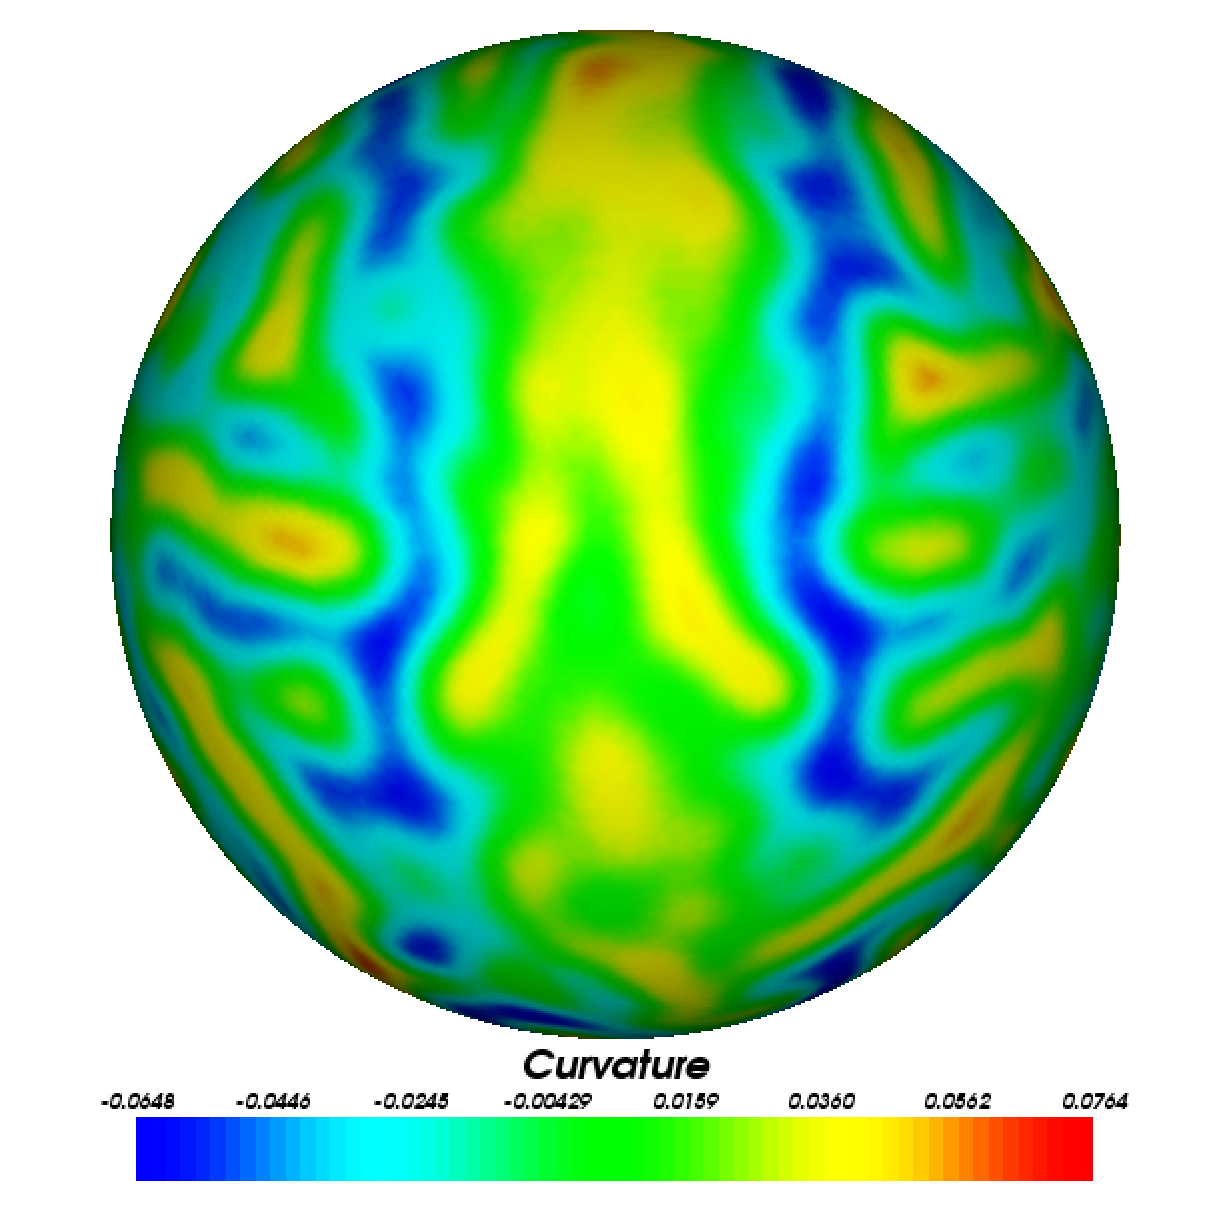
\includegraphics[%
  width=0.5\linewidth,
  keepaspectratio]{00111_smooth_128.ps}&
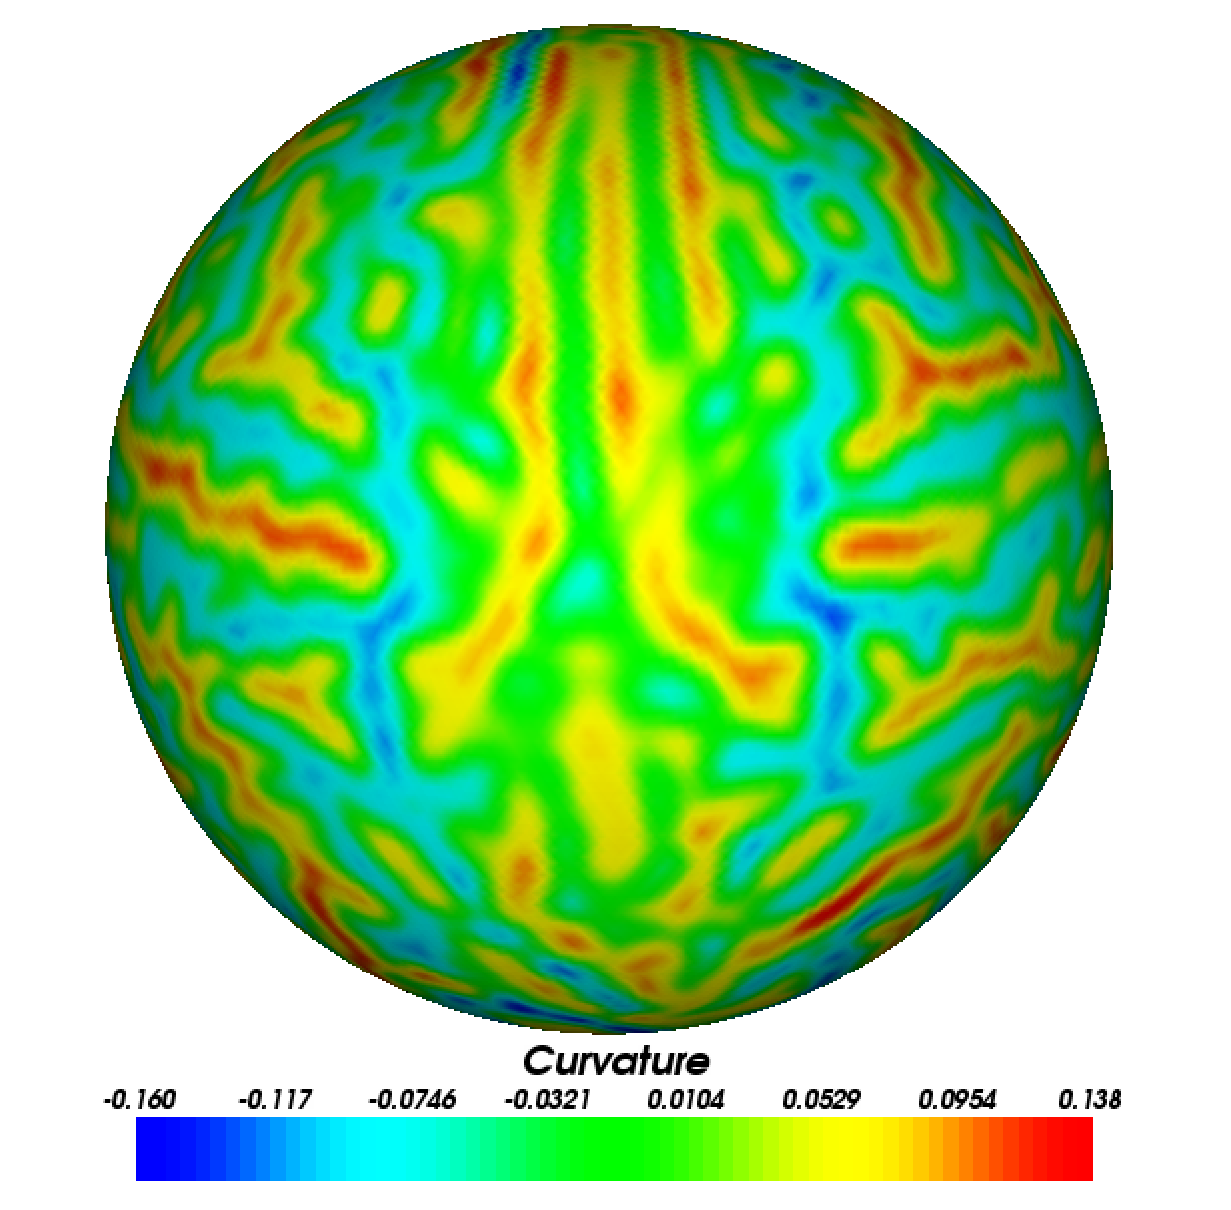
\includegraphics[%
  width=0.5\linewidth,
  keepaspectratio]{00111_smooth_32.ps}\tabularnewline
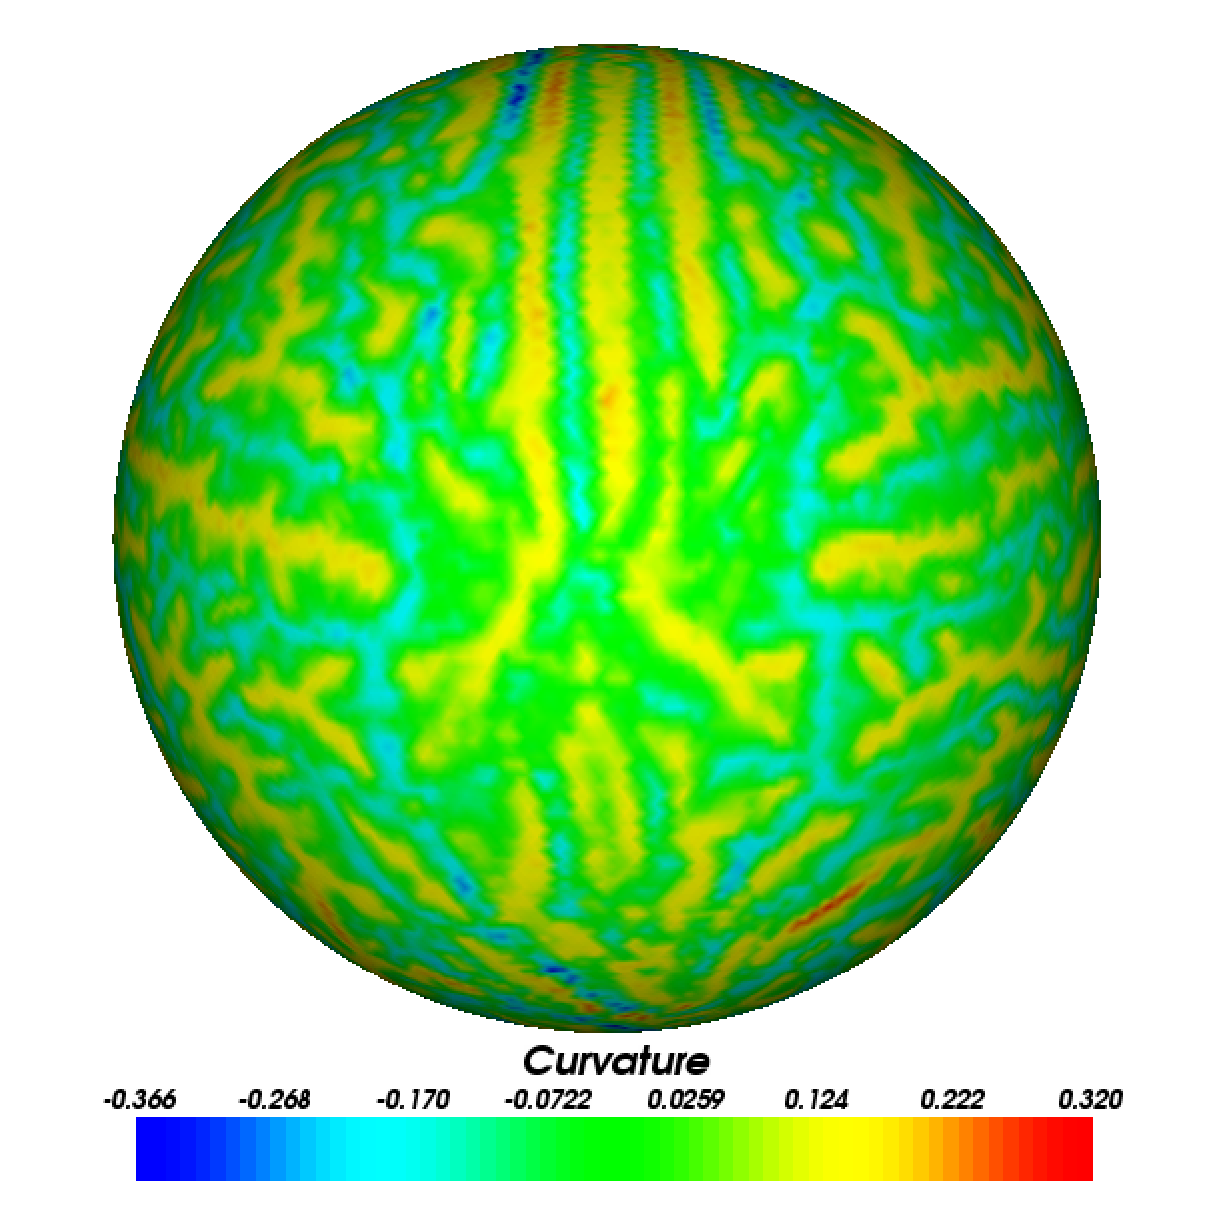
\includegraphics[%
  width=0.5\linewidth,
  keepaspectratio]{00111_smooth_8.ps}&
\includegraphics[%
  width=0.5\linewidth,
  keepaspectratio]{00111_smooth_2.ps}\tabularnewline
\end{tabular}\end{center}


\subsection{Inner Loop}

The optimization perfomed at each step of the coarse-to-fine outer
loop is the two-step Algorithm \ref{alg:Two-Step-Registration}, which
we call the inner loop.


\subsubsection{Matching (Step 2)}

The data term is written as a sum of terms, one for each vertex, $\Phi_{D}(U)=\sum_{v}\phi^{v}(U)$.
Each term is based on the correlation coefficient similarity measure
\cite{roche00:max-likelihood}, that produces a value in range $[-1,1]$
with better match indicated by larger score. Since \noun{surftracc}
operates as a minimization, we need to invert this\[
\phi^{v}(U)=1-\phi_{CC}^{v}(U),\]
where $\phi_{CC}^{v}$ is the correlation coefficient evaluated between
a neighbourhood of $v$ on the source data and a neighbourhood of
$U(v)$ on the target data. 

Each neighbourhood is a spherical cap at the given centre point $p$,
where $p$ is either $v$ or $U(v)$. The correlation coefficient
is evaluated by sampling on a set of sample points in each neighbourhood.
The sample points are arranged on a disc of radius $R_{n}$ parallel
to the tangent plane at $p$, as illustrated below. 

\begin{center}\includegraphics[%
  width=1\linewidth]{similarity-neighbourhood.eps}\end{center}

The set of sample points are: the centre of the disc, 8 points equally
spaced around a circle of radius $R_{n}/2$, and 16 points equally
spaced on a circle of radius $R_{n}$. The disc radius is \begin{equation}
R_{n}=r_{n}d_{C},\label{eq:define-neighbourhood-radius}\end{equation}
 where $r_{n}$ is a user-specified radius factor, and $d_{C}$ sets
the distance scale based on the coarseness of the control mesh. The
value of $d_{C}$ is the distance, projected to the disc, from the
centre of the cap to a neighbouring control mesh vertex. In other
words, $d_{C}$ is the length of a typical control mesh edge after
projecting to the disc. The value of $R_{n}$ must be no greater than
1, so $r_{n}\le1/d_{C}$.

The penalty $\Psi$ is also written as a sum over nodes of the control
mesh, $\Psi(T-U)=a\sum_{v}\psi(||T(v)-U(v)||)$. The penalty function
$\psi$ is designed so that $U(v)$ is restricted to the hemisphere
centred on $T(v)$. This is easily done by choosing $\psi$ such that
it becomes infinite when the angle between $T(v)$ and $U(v)$ reaches
$\pi/2$. 

With the search space restricted to a hemisphere, it can be parameterized
using two variables, by projecting the points on the sphere to the
tangent plane at $T(v)$. Thus, $U(v)$ is obtained using a two-dimensional
unconstrained optimization. Points $T(v)$ and $U(v)$ are projected
to this disc and $r$ is defined as the distance between the projected
points as illustrated.

\begin{center}\includegraphics[%
  width=1\linewidth]{search-neighbourhood.eps}\end{center}

The penalty is a logarithmic barrier function \cite{nocedal99:numerical-optimization},
$\psi=-\log(1-r^{2}/R_{s}^{2})$, which has the effect of constraining
the search for $U(v)$ to points with $r<R_{s}$. The disc radius
is \begin{equation}
R_{s}=r_{s}d_{T},\label{eq:define-search-radius}\end{equation}
 where $r_{s}$ is a user-specified search radius factor, and $d_{T}$
sets the distance scale based on the control mesh. The value of $d_{T}$
is the distance, projected to the disc, between $T(v)$ and $T(u)$
where $u$ is the control-mesh neighbour closest to $v$ on the target,
i.e. $||T(v)-T(u)||$ is minimum for all 1-ring neighbours $u$ of
$v$. The value of $R_{s}$ must be no greater than 1, so $r_{s}\le1/d_{T}$.

The objective function is designed to be separable so that the minimization
of \begin{equation}
\phi^{v}(U(v))+a\psi(||U(v)-T(v)||)\label{eq:objective-vertex-v-2d}\end{equation}
 is performed independently for each control mesh vertex $v$. Each
optimization is a 2-dimensional problem, parameterized by Cartesian
coordinates in the tangent plane at $T(v)$. The initial iterate is
$(0,0)$ which corresponds to $T(v)$, and is a feasible point since
it corresponds to $r=0$ so the barrier function $\psi$ is zero.
The optimization is performed using the Nelder-Mead downhill simplex
algorithm \cite{press88:numerical-recipes} as implemented in the
GNU Scientific Library \cite{galassi02:gsl-book}. The Nelder-Mead
simplex algorithm is chosen because it does not require derivatives
of the objective function \ref{eq:objective-vertex-v-2d}, which are
complicated due to the correlation coefficient data term in $\phi^{v}$. 


\subsubsection{Smoothing (Step 3)}

The smoothing, which is carried out in $\Rthree$, is a simple weighted
average of $U(v)$ and the centroid of its neighbourhood, \[
C(v)=\frac{1}{|N_{v}|}\sum_{u\in N_{v}}U(u),\]
where $N_{v}$ is the set of neighbours of $v$. The smoothed transformation
is given by \[
T(v)=\frac{U(v)+wC(v)}{||U(v)+wC(v)||},\]
where $w$ is a user-specified smoothing weight.


\subsection{Algorithm Parameters}

The user of this algorithm has four major parameters to specify: the
search radius $r_{s}$, the neighbourhood radius $r_{n}$, the penalty
ratio $a$, and the smoothing weight $w$. Note that the search radius
and neighbourhood radius are dimensionless quantities that multiply
a length set by the coarseness of the control mesh through Equations
\ref{eq:define-neighbourhood-radius} and \ref{eq:define-search-radius},
respectively. Thus $r_{s}$ and $r_{n}$ can be set to a fixed value
for all iterations of the outer coarse-to-fine loop, as are parameters
$a$ and $w$.


\section{Output}

The output is a map $T:\Stwo\rightarrow\Stwo$, specified in a piecewise
linear fashion by providing $T(v)$ for all vertices $v$ of the control
mesh. The transformation at vertex $v$ is a point $T(v)\in\Stwo$.
However, instead of storing the Euclidean coordinates for the point
$T(v)$, the triple $(h,\alpha,\beta)$ is stored where $h$ is a
halfedge (internally represented as a pointer) specifying the spherical
triangle of the target data mesh that contains $T(v)$ and $(\alpha,\beta)$
are the areal coordinates (along with $\gamma\equiv1-\alpha-\beta$)
locating $T(v)$ on the spherical triangle as illustrated.

\begin{center}\includegraphics{surfacepoint.eps}\end{center}

%% LyX 1.3 created this file.  For more info, see http://www.lyx.org/.
%% Do not edit unless you really know what you are doing.
\documentclass[10pt,letterpaper,twocolumn,english]{article}
\usepackage{ae}
\usepackage{aecompl}
\usepackage[T1]{fontenc}
\usepackage[latin1]{inputenc}
\usepackage{float}
\usepackage{amsmath}
\usepackage{graphicx}
\usepackage{amssymb}

\makeatletter

%%%%%%%%%%%%%%%%%%%%%%%%%%%%%% LyX specific LaTeX commands.
\newcommand{\noun}[1]{\textsc{#1}}
%% Because html converters don't know tabularnewline
\providecommand{\tabularnewline}{\\}
\floatstyle{ruled}
\newfloat{algorithm}{tbp}{loa}
\floatname{algorithm}{Algorithm}

%%%%%%%%%%%%%%%%%%%%%%%%%%%%%% User specified LaTeX commands.
\usepackage{url}

\newcommand{\inlinedef}[1]{\emph{#1}\index{#1}\glossary{#1}}
\newcommand{\sphericaltri}{\textcircled{$\triangle$}}

\usepackage{babel}
\makeatother
\begin{document}

\title{The Theory and Practice of Non-Rigid Surface Warping}


\author{Steven M. Robbins}

\maketitle

\newcommand{\Real}{\mathbb{R}}

\newcommand{\Rthree}{\mathbb{R}^{3}}

\newcommand{\Stwo}{\mathbb{S}^{2}}



\section{Introduction}

Surface registration is a procedure that produces a spatial mapping
from one surface, which we call the \emph{source} surface, to a second,
\emph{target}, surface. This manual is not a treatise on surface registration
(see, e.g. \cite{robbins03:phd}) but only documents the specific
theory and practice underlying \noun{surftracc}. 


\section{Input Data}

The input to surface registration is a pair of surfaces such as those
generated from a 3D MR image using software such as \noun{asp}/\noun{clasp}\cite{macdonald00:cortical-surfaces}.
In adition, a feature data function for each surface is required.


\subsection{Surface Description}

Each input surface must be a triangulated polyhedral surface, also
called a \emph{mesh}. Further, \noun{surftracc} assumes that the
surface has a very specific structure as follows.

First of all, \noun{surftracc} requires that the mesh represent
a topological sphere, i.e. a closed surface that bounds a finite volume
of space.

A common way to refine a mesh is by quadrisection, in which each triangle
is replaced by four triangles by joining the midpoints of the three
edges, as shown.

\begin{center}\includegraphics{quadrisection.eps}\end{center}

In addition to being a topological sphere, \noun{surftracc} requires
that the mesh graph be a repeated quadrisection of an icosahedron,
the graph with 20 triangular faces and 12 vertices each of degree
five. Each quadrisection increases the number of faces by a factor
of four. The following table shows the number of faces and vertices
produced by repeated quadrisection.

\begin{center}\begin{tabular}{|c|c|c|}
\hline 
\# Quadrisections&
\# Faces&
\# Vertices\tabularnewline
\hline
\hline 
0&
20&
12\tabularnewline
\hline 
1&
80&
42\tabularnewline
\hline 
2&
320&
162\tabularnewline
\hline 
3&
1280&
642\tabularnewline
\hline 
4&
5120&
2562\tabularnewline
\hline 
5&
20480&
10242\tabularnewline
\hline 
6&
81920&
40962\tabularnewline
\hline 
7&
327680&
163842\tabularnewline
\hline
\end{tabular}\end{center}

Note that ASP/CLASP outputs surfaces of the form required by \noun{surftracc}.


\subsection{Match Feature}

Along with each surface, we need data to determine how the surfaces
match. The basic idea is to define a scalar \emph{feature} function
on each surface such that a matching region on the source and target
have a similar feature pattern. The feature values needn't match exactly
since, as described below, we use a correlation similarity measure
to drive the optimization.

The feature function is defined in a piecewise-linear fashion by providing
the function value at each vertex. At other points on the surface,
the function is interpolated from the 3 values at the triangle vertices.
This interpolation is described in more detail later.

We next describe two geometric feature functions that can be used
for registration: mean curvature and crown distance transform.


\subsubsection{Curvature}

The mean surface curvature is a popular choice for match feature since
gyral crowns and sulcal fundii have curvature of different sign. So
matching curvature should match gyrus to gyrus and sulcus to sulcus.

This Figure shows the value of mean curvature evaluated (using \cite{taubin95:estimating-curvature})
at each vertex of the cortical surface.

\begin{center}\begin{tabular}{cc}
\includegraphics[%
  width=0.45\linewidth,
  keepaspectratio]{mean-cortex-top.ps}&
\includegraphics[%
  width=0.45\linewidth,
  keepaspectratio]{mean-sphere-top.ps}\tabularnewline
\end{tabular} \end{center}

Since sulcal fundi and gyral crowns have mean curvature of opposite
sign, registration based on matching mean curvature should tend to
match sulcus to sulcus and gyrus to gyrus. However, there is evidently
a lot of noise in the curvature map as well, due to small-scale oscillations
in the mesh vertex positions, so the data needs to be smoothed when
used for registration, either by smoothing the surface before computing
the curvature, or by directly averaging function values in a neighbourhood
of each vertex.


\subsubsection{Crown Distance Transform}

The intuition behind this feature, like that of mean curvature, is
that it is desirable to match points along the crown of a gyrus on
the source surface with points along the crown of a gyrus in the target
surface. Similarly, the fundus of a sulcus should match the fundus
of a sulcus. In contrast to matching by mean curvature, other points
on the bank of a sulcus are matched according to their fractional
distance towards the bottom of the sulcus, e.g. a vertex halfway down
the sulcus in the source mesh should match a point halfway down the
target sulcus.

Suppose vertex $v$ is located in a sulcus of the source mesh. Consider
two shortest geodesic paths, one from $v$ to the gyral crown and
the other from $v$ to the fundus. Let the length of the first of
these paths be $S(v)$ and let $S_{D}(v)$ be the sum of the two path
lengths. Distance $S_{D}(v)$ can be regarded as the depth of the
sulcus along a path through $v$. Let $R$ and $R_{D}$ be the analogous
distance functions for the target surface. The fractional depth of
vertex $v$ on the source mesh is $S(v)/S_{D}(v)$.

\begin{center}\includegraphics[%
  width=0.9\columnwidth,
  height=0.2\paperwidth,
  keepaspectratio]{fractional-depth.eps}\end{center}

The desired matching is to a point $T(v)$ on the target surface such
that $S(v)/S_{D}(v)\approx R(T(v))/R_{D}(T(v))$, or\begin{equation}
R(T(x))=\alpha(x)+\beta(x)S(x)+\epsilon(x),\label{eq:dt-matching-relation}\end{equation}
 where $\epsilon$ represents random noise, $\beta(x)=R_{D}(T(x))/S_{D}(x)$,
and $\alpha$ should be zero. However, $\alpha$ is left free to compensate
for practical difficulties in computing $S(x)$ and $R(x)$. Note
that points near to $v$ should have depth values close to $S_{D}(v)$
and similarly points near $T(v)$ should have depth values close to
$R_{D}(T(v))$. Assuming that $\alpha$ and $\beta$ are slowly-varying
functions, the maximum likelihood estimate for $T$ corresponds to
maximizing the regional correlation coefficient \cite{robbins03:phd}. 

Note that only the gyral crown distance functions, $S$ and $R$ appear
in Equation~\ref{eq:dt-matching-relation} and not $S_{D}$ and $R_{D}$.
Thus, the feature value stored at each vertex is the geodesic \emph{distance
transform} from a set of gyral {}``seed'' vertices, i.e. the length
of the shortest geodesic path from $v$ to a vertex in the seed set.


\paragraph{Seed Points}

The vertices chosen to be the seeds should in principle be all vertices
located on all the gyral crowns. We can identify gyral vertices with
the help of an \emph{$\alpha$-shape} \cite{edelsbrunner94:alpha-shapes},
a discrete geometry notion that can be considered as a relaxation
of the convex hull. The degree of relaxation is controlled by the
parameter $\alpha$ in the following manner. Let $S$ be a set of
points in $\Rthree$. Define an \emph{$\alpha$-ball}%
\footnote{The definition given here follows the Computational Geometry Algorithms
Library (CGAL) \cite{cgal-web}, as the implementation of $\alpha$-shape
provided by CGAL is used. In the original definition of Edelsbrunner
and M�cke, $\alpha$ is the radius of the $\alpha$-ball.%
} to be a closed ball of radius $\sqrt{\alpha}$, i.e. the point set
$\{ x\in\Rthree:||x-p||\le\sqrt{\alpha}\}$, for some $p\in\Rthree$.
The points of $S$ that form the vertices of the $\alpha$-shape of
$S$ are those that lie on the boundary of an $\alpha$-ball with
no point of $S$ on the interior of the $\alpha$-ball. Such vertices
are said to be \emph{$\alpha$-exposed.} Note that convex hull vertices
are always $\alpha$-exposed, since for every point $x$ on the boundary
of a convex set, there exists a ball of radius $\sqrt{\alpha}$ for
any value of $\alpha$ that intersects the convex set only at $x$.
Thus the vertices of the $\alpha$-shape with $\alpha=\infty$ are
the vertices of the convex hull. As $\alpha$ is decreased, more points
become $\alpha$-exposed until at $\alpha=0$ all points are $\alpha$-exposed. 

Using $\alpha$-balls of radius 10 mm (i.e. $\alpha=100$), a value
empirically chosen using visual inspection of the results, produces
good outlines of several major gyri. However, there are also vertices
in the point set lying underneath the brain on the arbitrary {}``cap''
through the brain stem which should not form part of the seed set;
these vertices are masked out as follows. The distance transform is
computed using the convex hull points as the seed vertices and any
vertex with a distance transform value greater than 35 (a value chosen
empirically) is removed from the set of vertices of the $\alpha$-shape.
The remaining vertices form the seed set used for the crown distance
transform feature.


\paragraph{Geodesic Distance}

The distance transform used in practice is an approximation to the
geodesic distance, as computing true geodesic distance is computationally
costly and difficult to code robustly \cite{lanthier01:approx-weighted-shortest-path}.
The approximation is computed using the mesh graph with the weight
for each edge set to the Euclidean length of the edge. An additional
vertex, $s$, is inserted and attached to each seed vertex with a
zero weight edge. Then Dijkstra's single-source shortest path algorithm
\cite{cormen90:intro-algorithms} is run with $s$ as the source vertex.
To improve the accuracy of the approximation the mesh is refined before
running Dijkstra's shortest path algorithm. First, $m$ equally-space
extra points are inserted on each edge, then a new edge is inserted
for each pair of extra points that either (i) are adjacent on an original
edge, or (ii) are on different edges both of which are incident to
a common (original) facet. The approximate shortest path computed
by this algorithm consists of line segments which are either an edge
of the original surface, or cross a facet of the original surface
as shown.

\begin{center}\includegraphics{approximate-path.eps}\end{center}

The crown distance transform from the final seed set is illustrated
below.

\begin{center}\begin{tabular}{cc}
\includegraphics[%
  width=0.4\columnwidth,
  height=0.15\paperwidth,
  keepaspectratio]{sphere-top.ps}&
\includegraphics[%
  width=0.4\columnwidth,
  height=0.15\paperwidth,
  keepaspectratio]{sphere-bottom.ps}\tabularnewline
Top&
Bottom\tabularnewline
\includegraphics[%
  width=0.4\columnwidth,
  height=0.15\paperwidth,
  keepaspectratio]{sphere-left.ps}&
\includegraphics[%
  width=0.4\columnwidth,
  height=0.15\paperwidth,
  keepaspectratio]{sphere-right.ps}\tabularnewline
Left&
Right\tabularnewline
\end{tabular}\end{center}


\section{Triangle Interpolation}

Both the feature data function described above and, ultimately, the
transformation $T$ are defined at mesh vertices and interpolated
across the rest of the surface. We pause to discuss this interpolation
before discussing the optimization used to search for $T$.


\subsection{Scalar Function Interpolation}

Suppose that for a function, $f$, a real value is associated with
each vertex of the mesh, as is the case for the feature function data.
Let $p$ be a point on the mesh and consider what value to assign
$f(p)$. 

If $p$ is a vertex, the vertex value is assigned. 

If $p$ is not a vertex, let $ABC$ be a triangle of the mesh that
contains $p$. There is a unique triple of real values $(\alpha,\beta,\gamma)$
with $\alpha+\beta+\gamma=1$ that satisfies $p=\alpha A+\beta B+\gamma C$.
This triple is known as the \emph{areal coordinates} of $p$ \cite[section 13.7]{coxeter69:intro-geometry}.
We use these values for interpolation, assigning $f(p)=\alpha f(A)+\beta f(B)+\gamma f(C)$.
It is clear that this choice of interpolation (a) is consistent with
the assigned values at vertices $A$, $B$, and $C$, and (b) gives
consistent values along a shared triangle edge no matter which triangle
is used for the interpolation.


\subsection{Triangulation Warping}


\subsubsection{Auxiliary Space}

While it is conceivable to define the mapping $T$ directly on the
input mesh, it is easier to use a simpler auxiliary space instead;
\noun{surftracc} uses the unit sphere. The source mesh, $M_{I}$,
is first mapped to the sphere using an invertible projection map,
$\Pi_{I}$. This projection is given implicitly by the fact that $M_{I}$
is constrained to be a repeated quadrisection of the icosahedron,
as discussed above. The target surface $M_{J}$ is similarly projected
to the sphere by $\Pi_{J}$. The registration algorithm then computes
$T:\Stwo\rightarrow\Stwo$ which, together with the two projection
operations, serves to define map between the two input surface meshes,
denoted $W:M_{I}\rightarrow M_{J}$ in the diagram.

\begin{center}\includegraphics[%
  width=1\columnwidth,
  keepaspectratio]{mappings.eps}\end{center}


\subsubsection{Triangulation Warping on the Sphere}

We discuss now how the sphere-to-sphere mapping, $T:\Stwo\rightarrow\Stwo$
is defined. The basic idea is that the source sphere is partitioned
into spherical triangles, and the mapping under $T$ is given for
each spherical triangle. 


\paragraph{Mapping one Triangle}

Let $A$, $B$, and $C$ be three points on the sphere $\Stwo$ that
are not coplanar with the origin. Using projection from the origin,
i.e. the mapping $x\mapsto x/||x||$, the planar triangle $ABC$ is
put into 1-1 correspondence with a triangular patch of $\Stwo$ bounded
by three shortest geodesics, from $A$ to $B$, from $B$ to $C$,
and from $C$ to $A$. Each geodesic bounding the patch is denoted
an \emph{edge arc}, and the triangular patch of $\Stwo$ is known
as the \emph{spherical triangle} $\sphericaltri ABC$. Given the 1-1
mapping between the planar triangle $\triangle ABC$ and the spherical
triangle $\sphericaltri ABC$, areal coordinates can be used to refer
to either $q=\alpha A+\beta B+\gamma C\in\triangle ABC$ or to $p=q/||q||\in\sphericaltri ABC$.

The mapping of $\sphericaltri ABC$ begins by specifying the positions
of the vertices under the mapping; define $A'\equiv T(A)$, $B'\equiv T(B)$,
and $C'\equiv T(C)$. Define a mapping from point $p$ in spherical
triangle $\sphericaltri ABC$ to point $T(p)$ in spherical triangle
$\sphericaltri A'B'C'$ as follows. First, project $p$ to point $q$
on the planar triangle $ABC$ and compute the areal coordinates of
$q$. We define the corresponding point $q'\in\triangle A'B'C'$ using
$q'\equiv\alpha A'+\beta B'+\gamma C'$. Finally, $q'$ is projected
to point on the sphere, denoted $p'$ and we define $T(p)$ to be
$p'$. 

\begin{center}\includegraphics[%
  width=1\columnwidth,
  keepaspectratio]{trianglemap-sphere.eps}\end{center}


\paragraph{Mapping the Entire Sphere}

In order to map the entire sphere, all we need is a partitioning of
the sphere into a set of non-overlapping spherical triangles. For
each triangle, we use the procedure just described to map it. Since
each point of the input sphere is contained in at least one triangle,
a mapping of the sphere is achieved. As is the case when interpolating
real values, the interpolation of $T$ is consistent at vertices and
along edges of each spherical triangle. The overall mapping $T$ is
1-1 and invertible if it satisfies certain conditions \cite{robbins03:phd}.
The main two conditions are that (a) the orientation of each spherical
triangle is preserved (i.e. the triangle is not {}``flipped'') and
(b) for each vertex, the cyclic ordering of its neighbouring vertices
is preserved.

Note that the partitioning of the source sphere is equivalent to finding
a simple triangulated mesh, denoted the \emph{control} mesh, inscribed
in the sphere. The input meshes to \noun{surftracc} provide such
a mesh due to the constraint that they be obtained by repeated quadrisection
of the icosahedron.


\section{Optimizing the Spatial Transformation}

Registration is generally cast in terms of an optimization problem,
in which we seek $T$ that will optimize the match of the feature
function defined on each surface. \noun{surftracc} uses a minimization
with a correlation coefficient-based objective function that penalizes
difference between the feature value at corresponding points on the
surfaces.

In addition, the objective function incorporates a \emph{regularization}
term that penalizes a transformation that is unlikely. Let $S$ and
$R$ be the feature functions on the source and target surfaces, respectively.
The objective function $\Phi$ is expressed as a sum \begin{equation}
\Phi(S,R,T)=\Phi_{D}(S,R,T)+\Phi_{R}(T),\label{eq:obj-is-data-plus-reg}\end{equation}
 and the optimization problem to solve becomes 

\[
T=\arg\min_{T'}\Phi(S,R,T').\]
 

As discussed in the previous section, $T$ is given by specifying
its value at each vertex. The transformation value is a point on $\Stwo$,
which takes two parameters to specify (e.g. latitude and longitude),
so the registration algorithm has two parameters to optimize per vertex.
With so many parameters to estimate (80k on a 40k mesh), it is important
to choose an effective optimization technique. 


\subsection{Two Step Non-Rigid Warping Algorithm}

The complexity is handled by separating the problem into a number
of smaller optimizations \cite{nocedal99:numerical-optimization},
one per vertex. To make this happen, both the data and regularization
terms in Equation \ref{eq:obj-is-data-plus-reg} must be \emph{separable,}
i.e. expressible as a sum of simpler terms. The parameters being optimized
should be partitioned amongst the terms and each term should involve
just a few of the parameters being optimized.

The data term, after discretization to evaluate it on the mesh, is
naturally separable into one term per mesh vertex $v$, involving
only the two values required to specify $T(v)$.

The regularization term can also be made separable by transforming
the problem into two interleaved minimizations. We modify the problem
by introducing a second transformation, $U$. A third term is introduced
into the objective function to link the transformations, resulting
in 

\begin{equation}
\Phi(T,U)=\Phi_{D}(U)+\Psi(T-U)+\Phi_{R}(T),\label{eq:two-step-objective-3d}\end{equation}
where $\Psi$ penalizes difference between $T$ and $U$; we might
use $\Psi(T-U)=\int||T-U||^{2}$, for example. After minimizing over
both $T$ and $U$, the transformation $T$ is returned as the final
solution. In other words, the registration problem solved is\[
\arg\min_{T}\Phi'(T),\]
where \[
\Phi'(T)=\arg\min_{U}\Phi(T,U).\]


The new objective function, Equation \ref{eq:two-step-objective-3d},
has twice as many variables as the original objective function, $\Phi_{D}+\Phi_{R}$.
The registration algorithm proceeds in a sequence of {}``half iteration''
steps. One half iteration fixes the variables that define $T$ while
optimizing $U$ \begin{equation}
U=\arg\min_{U'}\Phi(T,U')=\arg\min_{U'}\Phi_{D}(U')+\Psi(T-U').\label{eq:two-step-U}\end{equation}
The next half iteration fixes the variables that define $U$ while
optimizing $T$\begin{equation}
T=\arg\min_{T'}\Phi(T',U)=\arg\min_{T'}\Psi(T'-U)+\Phi_{R}(T').\label{eq:two-step-T}\end{equation}
 The first step (Expression \ref{eq:two-step-U}) can be seen as finding
a transformation, $U$, that matches the data while remaining close
to the previous solution, $T$ by virtue of $\Psi$. The second step
(Expression \ref{eq:two-step-T}) can be seen as regularizing the
transformation $U$ to produce a smoother transformation $T$. This
is summarized in Algorithm \ref{alg:Two-Step-Registration}. %
\begin{algorithm}

\caption{\label{alg:Two-Step-Registration}Two-Step Registration.}

\begin{enumerate}
\item Set $T$ to initial estimate.
\item Minimize $\Phi_{D}(U)+\Psi(T-U)$, where the term $\Psi$ penalizes
deviation of $U$ from $T$.
\item Set $T$ to be the smoothed version of $U$.
\item Repeat steps 2-3 until done.
\end{enumerate}

\end{algorithm}
 One cost of broadening the criterion for the two steps is that the
resulting algorithm may no longer be interpretable as a minimization
problem. 

One of the advantages of this algorithm is that $\Psi$ can easily
be chosen to be separable so that, when $\Phi_{D}$ is also separable,
the optimization in step 2 is separable. Step 3, though not necessarily
separable, requires only linear time and space. So the overall algorithm
is tractable.


\subsection{Coarse-to-Fine Hierarchy}

Non-rigid registration of the sort implemented here is almost universally
performed with multiple {}``resolutions'' of the transformation.
\noun{surftracc} implements this idea by running Algorithm~\ref{alg:Two-Step-Registration}
on a coarse control mesh of 1280 triangles (a three-fold quadrisection
of the icosahedron). The control mesh is then refined using quadrisection,
the mapping function $T$ is interpolated onto the new control mesh,
and Algorithm~\ref{alg:Two-Step-Registration} is run again.

As previously discussed, the input surface mesh is a quadrisection
of the icosahedron, typically six-fold (81920 triangles). The control
mesh begins as a three-fold quadrisection of the \emph{same} icosahedron.
Thus, after a number of repeated refine and registration steps, the
control mesh will exactly coincide with the input surface mesh. The
registration terminates at this point with the value of $T$ specified
for each vertex of the input mesh.


\subsubsection{Initial Surface Mapping}

In principle, the initial mapping of the coarsest control mesh should
be obtained by a low-dimensional warping, e.g. searching for the optimal
rotation of the sphere. However, the current implementation of \noun{surftracc}
assumes the user has done this as a preprocessing step. Typically
this is achieved by obtaining both the source and target surfaces
using \noun{asp} from MR images that are initially registered using
a 9-parameter affine transformation to a common target. Since the
MR images are aligned, a given vertex $v$ of the initial mesh tends
to end up in a nearly homologous location on each image \cite{macdonald00:cortical-surfaces}.
This means that the initial transformation on the coarsest control
mesh can simply be set to the identity mapping. 


\subsubsection{Data Refinement}

When the feature value map requires smoothing so as to reduce noise,
the smoothing is typically done in a coarse-to-fine manner in step
with the control mesh refinement. The coarse control mesh is used
with heavily-smoothed data, with the amount of smoothing being reduced
after each level of the hierarchy.

One simple method for smoothing is as follows. Let $D(v)$ denote
the data value at vertex $v$. The data smoothing replaces, in parallel
for all $v$, $D(v)$ by \begin{equation}
(D(v)+a\sum_{u\in N_{v}}D(u))/\alpha,\label{eq:smooth-scalars}\end{equation}
where $N_{v}$ is the set of neighbours of $v$, $\alpha=1+a|N_{v}|$
is a scaling factor to ensure the weights add to 1, and $a$ is a
constant. The smoothing operation is iterated, say, 128 times at the
coarsest level of control mesh, 32 for the next, then 8, and finally
twice at the level of the finest control mesh. The result of such
smoothing the mean curvature data term shown below. 

\begin{center}\begin{tabular}{cc}
\includegraphics[%
  width=0.5\linewidth,
  keepaspectratio]{00111_smooth_128.ps}&
\includegraphics[%
  width=0.5\linewidth,
  keepaspectratio]{00111_smooth_32.ps}\tabularnewline
\includegraphics[%
  width=0.5\linewidth,
  keepaspectratio]{00111_smooth_8.ps}&
\includegraphics[%
  width=0.5\linewidth,
  keepaspectratio]{00111_smooth_2.ps}\tabularnewline
\end{tabular}\end{center}


\subsection{Inner Loop}

The optimization perfomed at each step of the coarse-to-fine outer
loop is the two-step Algorithm \ref{alg:Two-Step-Registration}, which
we call the inner loop.


\subsubsection{Matching (Step 2)}

The data term is written as a sum of terms, one for each vertex, $\Phi_{D}(U)=\sum_{v}\phi^{v}(U)$.
Each term is based on the correlation coefficient similarity measure
\cite{roche00:max-likelihood}, that produces a value in range $[-1,1]$
with better match indicated by larger score. Since \noun{surftracc}
operates as a minimization, we need to invert this\[
\phi^{v}(U)=1-\phi_{CC}^{v}(U),\]
where $\phi_{CC}^{v}$ is the correlation coefficient evaluated between
a neighbourhood of $v$ on the source data and a neighbourhood of
$U(v)$ on the target data. 

Each neighbourhood is a spherical cap at the given centre point $p$,
where $p$ is either $v$ or $U(v)$. The correlation coefficient
is evaluated by sampling on a set of sample points in each neighbourhood.
The sample points are arranged on a disc of radius $R_{n}$ parallel
to the tangent plane at $p$, as illustrated below. 

\begin{center}\includegraphics[%
  width=1\linewidth]{similarity-neighbourhood.eps}\end{center}

The set of sample points are: the centre of the disc, 8 points equally
spaced around a circle of radius $R_{n}/2$, and 16 points equally
spaced on a circle of radius $R_{n}$. The disc radius is \begin{equation}
R_{n}=r_{n}d_{C},\label{eq:define-neighbourhood-radius}\end{equation}
 where $r_{n}$ is a user-specified radius factor, and $d_{C}$ sets
the distance scale based on the coarseness of the control mesh. The
value of $d_{C}$ is the distance, projected to the disc, from the
centre of the cap to a neighbouring control mesh vertex. In other
words, $d_{C}$ is the length of a typical control mesh edge after
projecting to the disc. The value of $R_{n}$ must be no greater than
1, so $r_{n}\le1/d_{C}$.

The penalty $\Psi$ is also written as a sum over nodes of the control
mesh, $\Psi(T-U)=a\sum_{v}\psi(||T(v)-U(v)||)$. The penalty function
$\psi$ is designed so that $U(v)$ is restricted to the hemisphere
centred on $T(v)$. This is easily done by choosing $\psi$ such that
it becomes infinite when the angle between $T(v)$ and $U(v)$ reaches
$\pi/2$. 

With the search space restricted to a hemisphere, it can be parameterized
using two variables, by projecting the points on the sphere to the
tangent plane at $T(v)$. Thus, $U(v)$ is obtained using a two-dimensional
unconstrained optimization. Points $T(v)$ and $U(v)$ are projected
to this disc and $r$ is defined as the distance between the projected
points as illustrated.

\begin{center}\includegraphics[%
  width=1\linewidth]{search-neighbourhood.eps}\end{center}

The penalty is a logarithmic barrier function \cite{nocedal99:numerical-optimization},
$\psi=-\log(1-r^{2}/R_{s}^{2})$, which has the effect of constraining
the search for $U(v)$ to points with $r<R_{s}$. The disc radius
is \begin{equation}
R_{s}=r_{s}d_{T},\label{eq:define-search-radius}\end{equation}
 where $r_{s}$ is a user-specified search radius factor, and $d_{T}$
sets the distance scale based on the control mesh. The value of $d_{T}$
is the distance, projected to the disc, between $T(v)$ and $T(u)$
where $u$ is the control-mesh neighbour closest to $v$ on the target,
i.e. $||T(v)-T(u)||$ is minimum for all 1-ring neighbours $u$ of
$v$. The value of $R_{s}$ must be no greater than 1, so $r_{s}\le1/d_{T}$.

The objective function is designed to be separable so that the minimization
of \begin{equation}
\phi^{v}(U(v))+a\psi(||U(v)-T(v)||)\label{eq:objective-vertex-v-2d}\end{equation}
 is performed independently for each control mesh vertex $v$. Each
optimization is a 2-dimensional problem, parameterized by Cartesian
coordinates in the tangent plane at $T(v)$. The initial iterate is
$(0,0)$ which corresponds to $T(v)$, and is a feasible point since
it corresponds to $r=0$ so the barrier function $\psi$ is zero.
The optimization is performed using the Nelder-Mead downhill simplex
algorithm \cite{press88:numerical-recipes} as implemented in the
GNU Scientific Library \cite{galassi02:gsl-book}. The Nelder-Mead
simplex algorithm is chosen because it does not require derivatives
of the objective function \ref{eq:objective-vertex-v-2d}, which are
complicated due to the correlation coefficient data term in $\phi^{v}$. 


\subsubsection{Smoothing (Step 3)}

The smoothing, which is carried out in $\Rthree$, is a simple weighted
average of $U(v)$ and the centroid of its neighbourhood, \[
C(v)=\frac{1}{|N_{v}|}\sum_{u\in N_{v}}U(u),\]
where $N_{v}$ is the set of neighbours of $v$. The smoothed transformation
is given by \[
T(v)=\frac{U(v)+wC(v)}{||U(v)+wC(v)||},\]
where $w$ is a user-specified smoothing weight.


\subsection{Algorithm Parameters}

The user of this algorithm has four major parameters to specify: the
search radius $r_{s}$, the neighbourhood radius $r_{n}$, the penalty
ratio $a$, and the smoothing weight $w$. Note that the search radius
and neighbourhood radius are dimensionless quantities that multiply
a length set by the coarseness of the control mesh through Equations
\ref{eq:define-neighbourhood-radius} and \ref{eq:define-search-radius},
respectively. Thus $r_{s}$ and $r_{n}$ can be set to a fixed value
for all iterations of the outer coarse-to-fine loop, as are parameters
$a$ and $w$.


\section{Output}

The output is a map $T:\Stwo\rightarrow\Stwo$, specified in a piecewise
linear fashion by providing $T(v)$ for all vertices $v$ of the control
mesh. The transformation at vertex $v$ is a point $T(v)\in\Stwo$.
However, instead of storing the Euclidean coordinates for the point
$T(v)$, the triple $(h,\alpha,\beta)$ is stored where $h$ is a
halfedge (internally represented as a pointer) specifying the spherical
triangle of the target data mesh that contains $T(v)$ and $(\alpha,\beta)$
are the areal coordinates (along with $\gamma\equiv1-\alpha-\beta$)
locating $T(v)$ on the spherical triangle as illustrated.

\begin{center}\includegraphics{surfacepoint.eps}\end{center}

\input{theory.bbl}
\end{document}

\end{document}

\end{document}

\end{document}
